%%%%%%%%%%%%%%%%%%%%%%%%%%%%%%%%%%%%%%%%%%%%%%%%%%%%%%%%%%%%%%%%%%% 
%                                                                 %
%                            ROOT FILE                            %
%                                                                 %
%%%%%%%%%%%%%%%%%%%%%%%%%%%%%%%%%%%%%%%%%%%%%%%%%%%%%%%%%%%%%%%%%%% 
%
%  Run LaTeX or pdfLaTeX on this file to produce your thesis.
%  To produce the abstract title page followed by the abstract,
%  see the file abstitle-phd.tex or abstitle-mas.tex.
%
%%%%%%%%%%%%%%%%%%%%%%%%%%%%%%%%%%%%%%%%%%%%%%%%%%%%%%%%%%%%%%%%%%%
\documentclass[chap]{rpi_thesis}  
% Use the first command below if you want captions over 1 line indented. A side
% effect of this is to remove the use of bold for captions (thesis default).
% To restore bold, also include the second line below.
\usepackage[hang]{caption}      % to indent subsequent lines of captions
\renewcommand{\captionfont}{\bfseries} % bold caption (needed with caption 
                                       % package to restore boldface.)                       

\captionsetup[algorithm]{labelsep=colon}

\usepackage{graphics}
\usepackage{graphicx}
\usepackage{url} 
\urlstyle{rm}

% For algorithms
\usepackage{algpseudocode}
\usepackage[chapter]{algorithm}

\renewcommand{\algorithmicrequire}{\textbf{Input:}}
\renewcommand{\algorithmicensure}{\textbf{Output:}}

% For code
\usepackage{listings}
\renewcommand*{\lstlistlistingname}{LIST OF LISTINGS}

% For equations 
\usepackage{amsmath}
\usepackage{amsfonts}
\usepackage{amssymb}

\renewcommand{\vec}[1]{\mathbf{#1}}

% For rotating in the tables
\usepackage{rotating} 
\usepackage[T1]{fontenc}

% To make the text tighter
% \usepackage{microtype}

% % For hyperreffing
\usepackage{hyperref}
% \usepackage[backref]{hyperref}
\hypersetup{
    unicode=false,          % non-Latin characters in Acrobats bookmarks
    pdftoolbar=true,        % show Acrobats toolbar?
    pdfmenubar=true,        % show Acrobats menu?
    pdffitwindow=true,      % page fit to window when opened
    pdftitle={My title},    % title
    pdfauthor={Author},     % author
    pdfsubject={Subject},   % subject of the document
    pdfnewwindow=true,      % links in new window
    pdfkeywords={keywords}, % list of keywords
    colorlinks=true,       % false: boxed links; true: colored links
    linkcolor=black,          % color of internal links
    citecolor=black,        % color of links to bibliography
    filecolor=black,      % color of file links
    urlcolor=black          % zcolor of external links
}
       
% TO CITE STUFF
\newcommand{\ignore}[1]{}
\newcommand{\nobibentry}[1]{{\let\nocite\ignore\bibentry{#1}}}
% apsrev entries in the text need definitions of these commands
\newcommand{\bibfnamefont}[1]{#1}
\newcommand{\bibnamefont}[1]{#1}
\newcommand{\Argmin}{\operatornamewithlimits{argmin}}
%\usepackage{natbib}
\usepackage{cite}
\usepackage{listings}
\usepackage{color}
\usepackage[toc,page]{appendix}
\usepackage{float}
\definecolor{dkgreen}{rgb}{0,0.6,0}
\definecolor{gray}{rgb}{0.5,0.5,0.5}
\definecolor{mauve}{rgb}{0.58,0,0.82}
\lstset{frame=tb,
  language=c, 
  aboveskip=3mm,
  belowskip=3mm,
  showstringspaces=false,
  columns=flexible,
  basicstyle={\small\ttfamily},
  numbers=none,
  numberstyle=\tiny\color{gray},
  keywordstyle=\color{blue},
  commentstyle=\color{dkgreen},
  stringstyle=\color{mauve},
  breaklines=true,
  breakatwhitespace=true
  tabsize=3
}

\renewcommand{\topfraction}{0.9}
\renewcommand{\bottomfraction}{0.8}

\setcounter{topnumber}{2}
\setcounter{bottomnumber}{2}
\setcounter{totalnumber}{4}

\renewcommand{\floatpagefraction}{0.8}


\begin{document}
% TO GET THE IEEE STANDARD RIGHT
%\bstctlcite{IEEE_Thing}
 
%%%%%%%%%%%%%%%%%%%%%%%%%%%%%%%%%%%%%%%%%%%%%%%%%%%%%%%%%%%%%%%%%%% 
%                                                                 %
%                            TITLE PAGE                           %
%               Master's Thesis or Master's Project               %
%                                                                 %
%%%%%%%%%%%%%%%%%%%%%%%%%%%%%%%%%%%%%%%%%%%%%%%%%%%%%%%%%%%%%%%%%%% 
%  This file produces the title page, copyright page (if requested)
%  and the Table of Contents, List of Figures and List of Tables.
% 
%  To produce the abstract title page followed by the abstract,
%  see the template file, "abstitle-mas.tex"
%%%%%%%%%%%%%%%%%%%%%%%%%%%%%%%%%%%%%%%%%%%%%%%%%%%%%%%%%%%%%%%%%%%

% Supply information for use on title page:    
\thesistitle{\bf Multi-user Non-linear Adaptive Magnification for Satellite Imagery and Graph Networks}
\author{Sean Christopher Kim}        
\degree{Master of Science} 
\department{Computer Science} % provide your area of study here; e.g.,
%  "Mechanical Engineering", "Nuclear Engineering", "Physics", etc.
   
\signaturelines{3}
\projadviser{Barbara Cutler} % For a masters project use \projadviser instead
%of \thadviser,
\memberone{Charles Stewart}        
\membertwo{David Mendon\c{c}a}
%\memberthree{Aristotle} % must change signaturelines to 4 if using this 4 members

\submitdate{July 2014\\(For Graduation August 2014)}        
%\copyrightyear{2013}   % if omitted, current year is used.        

% Print titlepage and other prefatory material:   
\titlepage     
%\copyrightpage         %optional           
\tableofcontents        
\listoftables          %required if there are tables
\listoffigures         %required if there are figures
%\lstlistoflistings

   % titlepage material for Master's thesis or project
%%%%%%%%%%%%%%%%%%%%%%%%%%%%%%%%%%%%%%%%%%%%%%%%%%%%%%%%%%%%%%%%%%% 
%                                                                 %
%                         ACKNOWLEDGEMENT                         %
%                                                                 %
%%%%%%%%%%%%%%%%%%%%%%%%%%%%%%%%%%%%%%%%%%%%%%%%%%%%%%%%%%%%%%%%%%% 
 
\specialhead{ACKNOWLEDGMENT}
I would like to thank the Department of Homeland Security Coastal Hazards Center at University of North Carolina at Chapel Hill for access to the resource infrastructure network used in this thesis. I would like to thank RPI's VP for Research for the seed grant used for funding ``Synthetic Environments for Investigating Organizational Resilience: An Application to Post-disaster Restoration of Critical Infrastructure Systems'' led by PIs David Mendon\,{c}a, Al Wallace, and Barb Cutler.

%%%%%%%%%%%%%%%%%%%%%%%%%%%%%%%%%%%%%%%%%%%%%%%%%%%%%%%%%%%%%%%%%%%
%                                                                 %
%                            ABSTRACT                             %
%                                                                 %
%%%%%%%%%%%%%%%%%%%%%%%%%%%%%%%%%%%%%%%%%%%%%%%%%%%%%%%%%%%%%%%%%%%

\specialhead{ABSTRACT}

% --------------------------------------------
% Introduction to the problem
% --------------------------------------------
Daylighting plays an important role in architecture, its creative and effective use offers aesthetics visuals, natural light, reduced energy consumption. 
Additional studies reviled many health benefits of having exposure to natural lighting over fluorescent lighting typical in office spaces. %TODO Cite
Due to these advantages of natural lighting, architects incorporate daylighting into the design of spaces such as offices, museums, and even residential estates. %TODO Cite
Daylighting is considered early on in the design process, where the use of sophisticated 3D modeling softwares can be considered excessive for the simple geometries considered in the early design phase.
Previous research has been conducted on an augmented reality physical sketching interface that allows users through placement of physical primitives to generate 3D models interactively for daylighting simulation.
User studies have shown this system, the Virtual Heliodon, to be useful in the creation of 3D spaces and analysis of daylighting performance.%TODO Cite
Despite the advantages offered, the physical setup of the Virtual Heliodon requires the use of many projectors, physical props, and a controlled lighting enviroment.

% --------------------------------------------
% Solution to the problem
% --------------------------------------------
While the Virtual Heliodon's augmented reality display offers users a collaborative space to share and experiment on architectural designs, the overhead of the setup of the Virtual Heliodon make it inaccessible to a potentially large user base that could provide us invaluable feedback on key algorithms and features that would improve daylighting analysis and design. 
We have come up with a web based interface that will be accessible to the general public and preserves the spirit the Virtual Heliodon.
This interface will offer most features available in the Virtual Heliodon in addition to features exclusive to the web application.%wording
Most importantly, we can reach a larger audience with our web based application to improve on the daylighting and sketch interpretation algorithms that are key to Virtual Heliodon.
% --------------------------------------------
% Do we have any final words?
% --------------------------------------------
In this thesis we describe in detail the features translated and exlusive to the web application of the Virtual Heliodon.
We will also discuss how we conducted a prototype study on the usabilty of our web application and the results from that study.

% --------------------------------------------
% Didn't make the CUT
% --------------------------------------------
\iffalse
Short list of what offer right now over physical heliodon
In addition using WebGL to render the visualization client side we can offer the user a view from any location in the scene without obscuring portions of the model.
Most importantly, we can reach a larger audience with our web based application to improve on the daylighting and sketch interpretation algorithms that are key to the Virtual Heliodon.
Despite the advantages offered, the physical setup of the Virtual Heliodon requires 4 or more HD projectors, a strong metal chaste, a high resolution camera,a large set of physical props, and a controlled lighting environment. 
\fi




 	% abstract

%%%%%%%%%%%%%%%%%%%%%%%%%%%%%%%%%%%%%%%%%%%%%%%%%%%%%%%%%%%%%%%%%%% 
%                                                                 %
%                           INTRODUCTION                          %
%                                                                 %
%%%%%%%%%%%%%%%%%%%%%%%%%%%%%%%%%%%%%%%%%%%%%%%%%%%%%%%%%%%%%%%%%%% 
 
% \specialhead{INTRODUCTION}
\chapter{INTRODUCTION}
\label{chapter:intro}

The Infrastructure Visualization application is a system for studying and training the decision making of emergency response personnel in times of crisis. The application is intended for situations requiring collaborative thinking among people with expertise in different fields. By displaying the data on a large central screen, the application is intended to foster discussion in solving complex problems which require a fast response time with limited resources. The data being shown by this application is difficult to understand in a
purely text based format. A solution to a possible disaster scenario may seem feasible at first, but without a complete picture of the data, the solution may not be comprehensive enough to solve the overall issue due to network interdependencies. To try and solve this problem, the interconnected data is represented visually as a network of nodes and edges with status information (OK, damaged, no service, etc.). The application should be easy to use, but also provide enough detail to adequately understand the underlying problem so that the participants can create an
adequate solution \cite{Mendonca2014}.

Satellite images of a region along with a graph network are displayed on the main screen. The nodes of the graph network represent the producers, consumers, and intermediary nodes of a particular resource, and the edges represent the connections between nodes which transmit the resource. The resources represented within the system are electricity, water, waste, and communications. For all of the resources besides communications, the nodes and edges are placed at their approximate
physical locations on the underlying satellite images. Some demand nodes are not tied to a particular resource, and are a census-based collections of data, which also do not have a specific geographic location. Each of the different resources has a color associated with it. To facilitate viewing information within this display, the nodes and edges can be expanded and collapsed to display relevant data. 

Figure~\ref{fig:mapview_example} shows an example image of the viewer application. The unexpanded nodes are currently drawn as circles, and the expanded nodes are drawn as squares to easily distinguish the data within the viewer. Expanded edges are simply wider than their unexpanded counterparts.

\begin{figure}[htp] \centering
    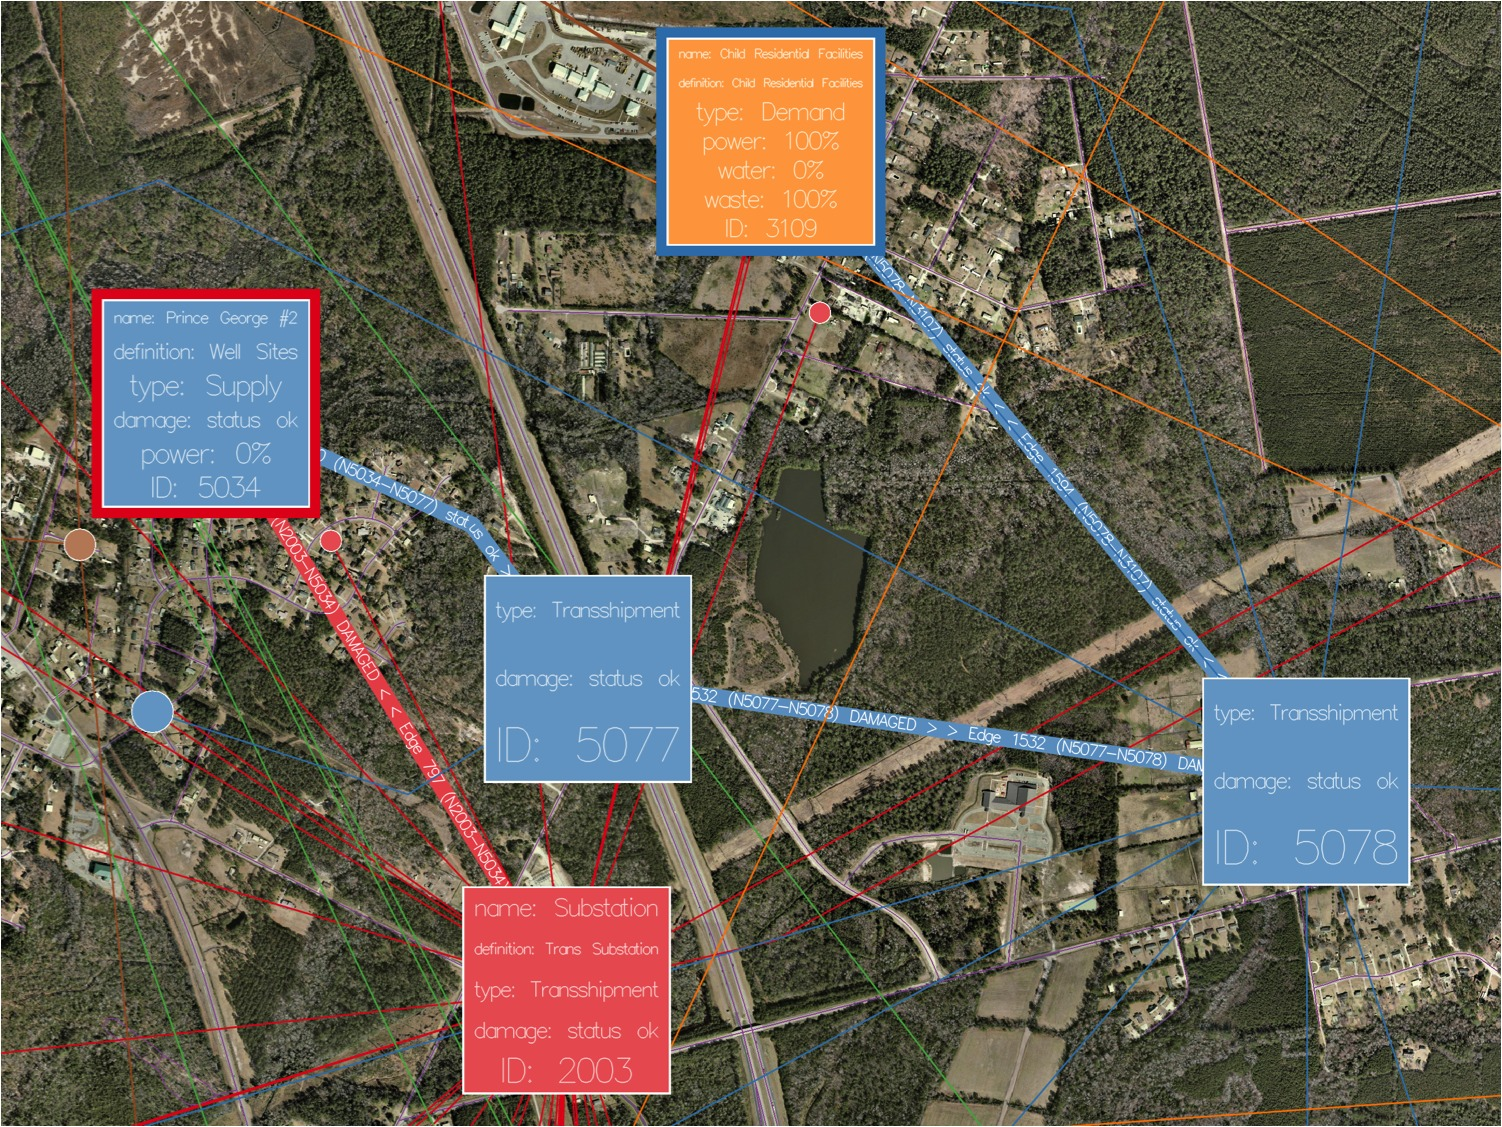
\includegraphics[width=0.8\linewidth]{img/mapview_example.jpg}
    \caption[Example Infrastructure Visualization]{This example screenshot shows an example scenario of a residential node lacking water,
    by following the network back to the supply node, we can deduce that the overall problem is twofold, a lack of power
    to the water supply node and a damaged water pipe - both must be addressed to restore water to the demand node.}
    \label{fig:mapview_example}
\end{figure}

When expanded, each node provides its id and name. If it is either a supply or transshipment node, it has a
corresponding status which indicates if it is currently supplying its resource to its edges. If a node requires a particular resource to function, it shows the current ratio of the supply and demand for that resource as a percentage. Edges show their current status: {\tt damaged} or {\tt status OK} as well as their ids and two corresponding node ids. If either a node or an edge is damaged, it is unable to transmit its resource.

When interacting with the system, users can toggle different parts of the display to simplify the data being presented. The underlying road network and satellite images can be turned off, as well as the nodes and edges of a particular resource. Users can also increase the level of detail of the application, effectively zooming in and out on the satellite images. This allows the users to see the a more detailed view of the satellite images and also reduces the number of graph elements on the screen. 

This entire application is designed to work with a system developed by Tyler Sammann and Chris Stuetzle, and which allows multiple users to interact with a system with mouse cursors and laser pointers \cite{Sammann2013}. These various input devices are generalized as cursors which have a generalized set of gestures, allowing for collaboration on a single screen between multiple users. In the context of the viewer application, this functionality allows the users to expand and
collapse the different graph elements, navigate to different areas of the map, change the global level of detail, and toggle the visibility of different elements as described above.

Systems that use multiple cursors are designed to foster collaborative problem solving and data exploration. Having multiple people interact with a system all at once allows people do explore different areas of the data set at the same time where normally a single person would control what everyone using the system sees. By having users work on a single shared screen instead of multiple displays, each individual user can more easily see what other people are looking at or
modifying.

Previous demonstrations of this application revealed that the current functionality was lacking a number of features that would allow for greater information visibility. Essentially, users are unable to view a particular region in a higher level of detail without possibly disturbing what the other users are viewing. Figure~\ref{fig:example_problem} presents an example of this issue.

\begin{figure}[htp] \centering
    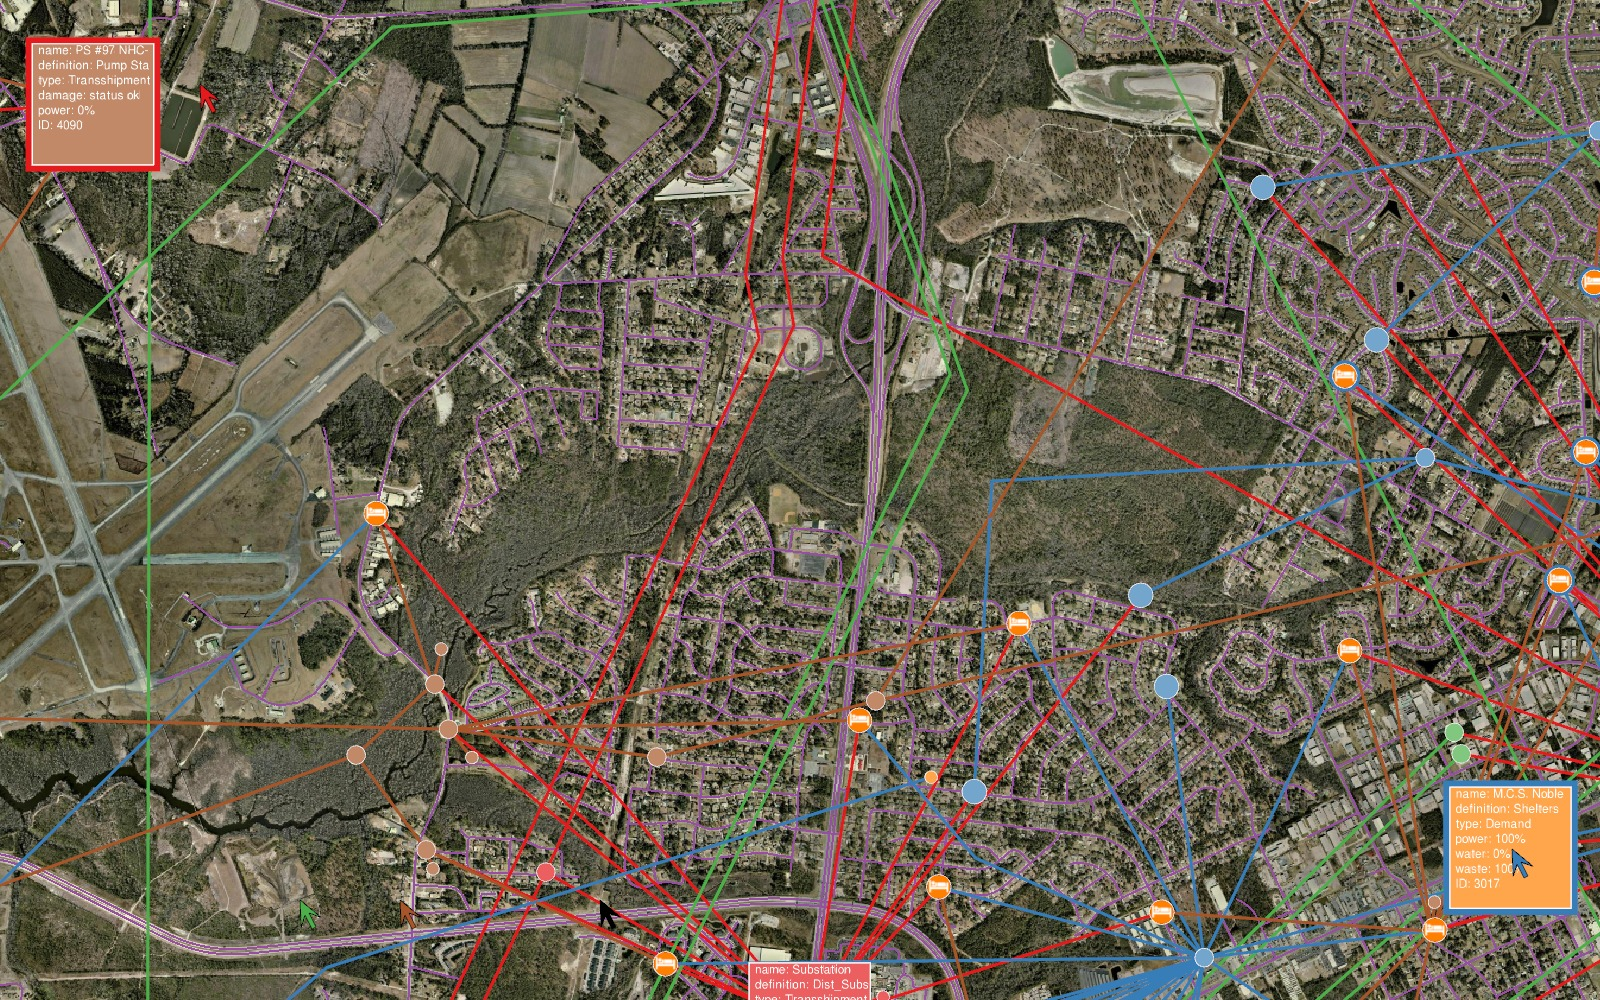
\includegraphics[width=150mm]{img/global_zoom_problem.jpg}
    \caption[Loss of Context]{This diagram shows a screenshot with two cursors in different regions of the application. The red arrow cursor is in the top left corner and the blue arrow cursor is in the bottom right corner. If either cursor performs a global zoom on their location to get more detail, the other cursor is unable to view their data.}
    \label{fig:example_problem}
\end{figure}

A system allowing for multiple areas of magnification when integrated with the previously mentioned multi-cursors could be useful in other contexts. If examining any sort of large graph based data set, being able to view different focal areas in higher detail would allow users to navigate data sets easier while still viewing the overall graph structure.

\section{Focus Plus Context}
\label{section:intro_fac}
Overview plus detail, zooming, and focus plus context are all methods within information visualization for displaying data. They each seek to present varying levels of data in a format that facilitates understanding. Overview plus detail visualizations are similar to physical maps of cities. The overall view of a city is shown on the big map, but a higher detail region of the city is shown in a separate, enclosed area (Figure~\ref{fig:louisiana}). This sort of visualization is easy to create, and is most
common for static media, as certain areas inherently require more detail than others when dealing with static data. Being able to interactively change the level of detail is the principle behind zooming visualizations (Figure~\ref{fig:google_maps}). This method is well suited for a single user looking to view different levels of detail at different points in time. It is also relatively easy to implement and does not cause distortions in the data being displayed. Focus plus context systems are useful for systems
where a user needs both a local and global view at the same time. Some loss of data can occur in these visualizations, but by using a single screen, the user does not need to mentally combine the data of a overview plus detail visualization. The first two formats separate data in two
different ways: overview plus detail interfaces separate data spatially, while zooming separates data temporally. Focus plus context uses a visual effect to display continuous information on a single screen \cite{Cockburn2008}. 

\begin{figure}[htp] \centering
    \includegraphics[width=0.8\linewidth]{img/1853_Louisiana.jpg}
    \caption[Overview Plus Detail]{This old map of Louisiana from 1853 showing a detailed view of a streets of New Orleans is an example of an overview plus detail visualization \cite{Mitchell1853}.}
    \label{fig:louisiana}
\end{figure}

\begin{figure}[htp] \centering
    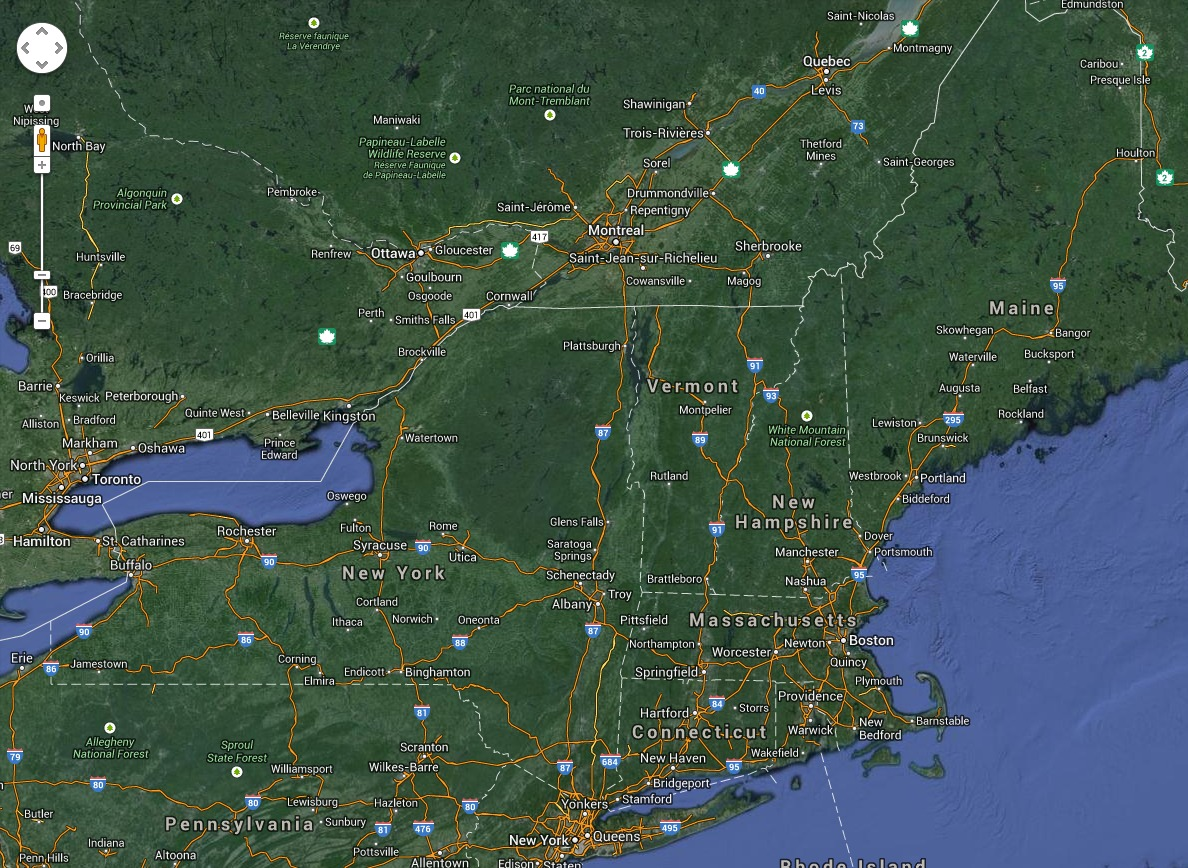
\includegraphics[width=0.8\linewidth]{img/zoom_interface.jpg}
    \caption[Zooming Interface]{An image of a common zooming interface for map data, Google Maps \cite{google_maps}.}
    \label{fig:google_maps}
\end{figure}

The goal of focus plus context interfaces is to reduce the cognitive load of managing multiple different views 
of a single system. Theoretically, this would improve user performance with regards to understanding and 
utilizing the data being presented. The foundation for the focus plus context interfaces was established by Furnas in 1986
\cite{Furnas1986}. He described a ``generalized fisheye view'' formula is described which 
calculates a user's ``degree of interest'' (\emph{DOI}) \cite{Furnas1986} (Equation~\ref{eq:furnas_doi}). The degree of interest, given a data element \emph{x} and focus \emph{y}, is the \emph{a priori interest} (API) in the data element minus the distance between the data element and the focus, \emph{D}.  The term fisheye in photography refers to a strong visual distortion which has an extremely wide angle. This photographic technique allows for more detail
in the resulting image by introducing distortion. The ``generalized fisheye view'' states that objects closer to the focal point are more important than ones further away, paralleling the fact that in a fisheye visualization, objects close to the focal point are less distorted.

\begin{equation}
    \label{eq:furnas_doi} 
    DOI(x, y) = API(x) - D(x,y)
\end{equation}

Focus plus context systems often perform some sort of distortion to present the data. Further work by Furnas within focus plus context systems highlighted the crucial fact that distortion based visualizations achieve a seamless display by requiring the user to understand that data is being modified in some manner \cite{Furnas2006}. All such distortions perform some sort of filtering of the data, as the distortion functions are presented on media with finite limitations. As information
gets further distorted, it is essentially filtered out, as it can no longer be discerned by the users. Distortion causes geometric distortion among the data, altering the positions and shapes, while maintaining topological continuity. This property is potentially desirable, as our application features satellite images, which should remain topologically continuous \cite{Furnas2006}. By remaining topologically continuous, users would still be able to discern the
relative distance between any two points on the map, as there are no regions of completely missing data.

Due to the nature of the data that we are working with, techniques that introduce some sort of distortion to achieve a focus plus context visualization are particularly relevant to the work presented in this thesis. Leung and Apperley provide an overview of such techniques\cite{Leung1994}. Among the relevant applications are the Polyfocal Display \cite{Kadmon1978}, the Perspective Wall \cite{Mackinlay1991}, and the Graphical Fisheye View \cite{Sarkar1992}. These techniques are further explored in
Chapter~\ref{chapter:previous_work}. Leung and Apperley classifies such techniques as magnification functions. The different functions can be further divided into techniques that have continuous magnification functions and those with noncontinuous piecewise functions. The different functions are unified into a single metaphor of a stretchable sheet on a rigid frame. By increasing the amount of data displayed in a single area, i.e. ``stretching'' the sheet to display information, other areas must ``shrink'' and display less data. The overall distortion effect that is then displayed is a result of the stretching and shrinking of the display.
This stretchable rubber metaphor holds up even for views with multiple foci, though it is paramount that the balance between magnification and demagnification is maintained, otherwise the ``frame'' of the sheet would be deformed. At the core of \cite{Leung1994} is the idea that all of these distortion techniques are similar, and are purely dependent upon a single magnification function. We will expand upon this idea of creating a magnification function for our visualization later on in Chapter~\ref{chapter:magnification}.

\section{Thesis Outline and Contributions}
\label{section:intro_outline}
As mentioned earlier, the first draft of the infrastructure visualization program has the ability to
recognize simultaneous input from multiple keyboards, computer mice, and lasers by individual participants, but only supported zooming on a global scale. This loss of information when performing a global zoom is a major hindrance to a system which should be used by multiple people at the same time. If diagnosing a central problem for discrete graph elements in different geographic regions, trying to get more information about the area around a node is impossible with the
current model without disrupting the other users. The main goals in designing this new system were to provide users the ability to view different regions of data at a variable level of detail without altering a majority of the
global context. Because this visualization may be viewed by people who are not directly interacting with the system, solutions that cause too much loss of global context should be avoided. If we change the global context, we run into the same issue of obscuring other regions of high importance. 

The first step in creating a solution which met our needs was the design and implementation of a proof-of-concept system. An investigation of previous methods of focus plus context visualizations was performed to formulate the design behind our solution, detailed in Chapter~\ref{chapter:previous_work}. The concepts learned from this system were then applied to the pre-existing application. The visualization required many changes to allow for the new feature to be implemented and a large bulk of time was spent on upgrading to modern OpenGL to also improve performance; these changes are detailed in Chapter~\ref{chapter:visualization}. Two separate magnification functions were created to affect both the satellite imagery and the
graph network. These functions, described in Chapter~\ref{chapter:magnification}, cause the graph elements to stay in the same geographic location, and are easily adjustable for different parameters. The speed of the new system with regards to rendering and performing the magnification functions was measured and recorded in Chapter~\ref{chapter:results}. Chapter~\ref{chapter:results} also includes an informal survey of untrained user responses was carried out to gauge the basic
usability of the new magnification system. Finally, further improvements and changes to the system are discussed in Chapter~\ref{chapter:future_work}.
 	% chapter 1

%%%%%%%%%%%%%%%%%%%%%%%%%%%%%%%%%%%%%%%%%%%%%%%%%%%%%%%%%%%%%%%%%%% 
%                                                                 %
%                           PREVIOUS WORK                         %
%                                                                 %
%%%%%%%%%%%%%%%%%%%%%%%%%%%%%%%%%%%%%%%%%%%%%%%%%%%%%%%%%%%%%%%%%%% 
 
% \specialhead{PREVIOUS WORK}
\chapter{PREVIOUS WORK}
\label{chapter:previous_work}

In this chapter, I will provide a more in-depth look at previous focus plus context systems and discuss the applicability of these techniques to our application.

\section{Focus Plus Context Visualizations}
\label{section:prev_fc_vis}

One of the earliest systems that tried to tackle the focus plus context problem was the \emph{Perspective Wall} presented by Mackinlay et al. \cite{Mackinlay1991}. This system was integrated with the \emph{Information Visualizer}, a system for visualizing data in 3D. The \emph{Perspective Wall} sought to imitate the nature of the human eye, by having a smooth integration between a focused area and the overall context. This system turns a 2D layout into a 3D wall system which contains
an area of detail surrounded by a distorted region. The \emph{Perspective Wall} had a flat region of high detail with regions surrounding it that were angled to match the field of view of the viewer. An image of the system is seen in Figure~\ref{fig:perspective_wall} showing the areas of magnification and demagnification. The focus of the application was to view information that was structured temporally, such as a filesystem. One of its greatest strengths was that it presented information in an intuitive manner. Unfortunately, while this work showed that such distortion techniques are helpful in facilitating understanding for the users, it is unsuited for our own purposes as this system performs a global distortion of the data and the metaphor does not easily extend to a system with different regions of focus.

\begin{figure}[htp] \centering
    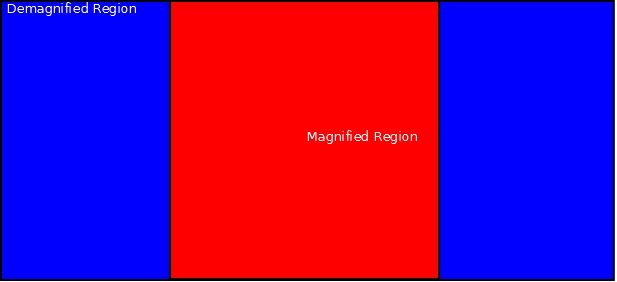
\includegraphics[width=0.45\linewidth]{img/Perspective_Wall.jpg}
    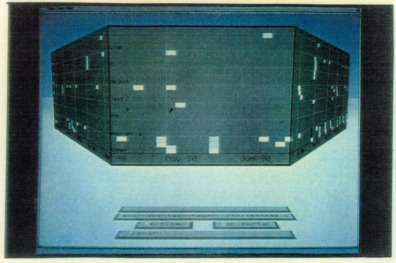
\includegraphics[width=0.45\linewidth]{img/perspective_wall_actual.jpg}
    \caption[Perspective Wall Diagram]{A figure showing the magnified and demagnified regions of the 
        \emph{Perspective Wall} \cite{Mackinlay1991}, and an image of the original system, created by Mackinlay 
        et al.. The blue regions are demagnified and represent the angled areas.}
    \label{fig:perspective_wall}
\end{figure}

Baudisch et al.\ attempted to display focus plus context information through the integration of different hardware into a single logical screen \cite{Baudisch2001}. This screen consists of a low resolution region for context and a high resolution area for detailed information. They achieve similar effects as a fisheye view, but avoid distortion with their hardware. The prototype constructed integrates a LCD screen with a projection screen; a diagram of the system along with an image
of the actual system is seen in Figure~\ref{fig:f_and_c}.  By having two distinct regions of resolution, they are able to maintain the overall
geometry of the displayed images. To achieve this effect, Baudisch et al.\ created a foam core projection screen with a cutout for a flat panel LCD monitor. A large portion of the work performed by Baudisch et al.\ was used for examining this system with different applications. Of particular note is their work with a map application for finding the shortest path between two cities. The display allowed for seeing both the surrounding geography and large highways between the cities, while
allowing the user to also view street-level detail for areas with densely packed information. A single application controls the rendering for both screens. The data is rendered at a resolution that would fill the projection screen if it was also high resolution. A region is clipped to fit the resolution of the LCD monitor, while the overall data is scaled to fit within the projection screen. This solution provides a distortion free visualization, but only has a single area of
higher resolution. Viewing different regions of the data is performed by moving the entire visualization, which is not well suited to interactively viewing different areas simultaneously, but works perfectly fine for a single user. Generating new hardware is also outside of the scope of this thesis, but the studies performed by Baudisch et al.\ provide useful insight. In a small user survey, it was found that the overall responsiveness of the application as well as the ability to see the bigger picture of the work was beneficial for users of the system.

\begin{figure}[htp] \centering
    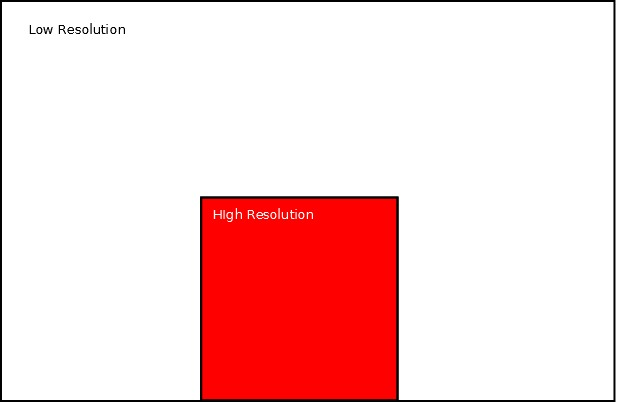
\includegraphics[width=0.45\linewidth]{img/f_and_c.jpg}
    \includegraphics[width=0.45\linewidth]{img/f_and_c_actual.jpg}
    \caption[Focus Plus Context Screen Diagram]{A figure showing the areas of high and low resolution images of 
    the focus plus context \cite{Baudisch2001} system created by Baudisch et al.. The red region is the LCD screen and the white area is the 
    projector screen.}
    \label{fig:f_and_c}
\end{figure}

Following their previous work, a formal study of the benefits of focus plus context displays was performed by Baudisch et al. Three different interfaces were evaluated with a number of different tasks to discover what display techniques were most helpful for completing said tasks \cite{Baudisch2002}. The focus plus context system described previously was compared with a zoom plus pan interface using a single screen and a overview plus detail interface using two monitors. All of the displays had approximately the same number of pixels between them. To further attempt to control for any extra space affecting the result of the experiment, the overview screen in the overview plus detail interface was constrained to the same size as the context of the focus plus context interface, while normally it would show the entirety of whatever dataset is being observed. There were two different types of tasks asked of the participants, the first was a static view where the users had to either
verify connections on a circuit board or find the closest hotel to a given point, and the second was a dynamic application where users were tasked with avoiding rocks and nails in a simple simulation. It was hypothesized and discovered that the focus plus context interface was the most helpful for performing both types of tasks. These results are promising for the infrastructure visualization, it suggests that a view providing a seamless integration between global and local data is most helpful in performing tasks which require both types of data. 

Gansner et al.\ describe a method for rendering sets of data with millions of nodes \cite{Gansner2005}. Their method, which they name ``Topological Fisheye'', follows the general principle given by Furnas et al.\ in  by having a detailed region around a focus with less information in other areas \cite{Furnas1986}. To reduce the amount of data in areas
out of focus, they create approximations of the original graph. When an area comes into focus, a hybrid graph is constructed by combining the various different approximations based on the distance from the focal point. To simplify the graph, they generate a proximity graph using either Delauney triangulation or a relative neighborhood graph and combine the results with the original edges of the graph to form a candidate set S. This set is then filtered by maximizing a weighted sum
of various measurements of the two points to be collapsed. The methods described in this construction are definitely applicable to future versions of the infrastructure visualization. As our data set grows, we may need to first simplify our graph data to filter out less important nodes. This filtered data could then be further transformed by a geometric transformation. A pure application of this would not adequately modify the underlying satellite images of our graph network.

\section{Geometric Transformations}
\label{section:prev_geometric_transformations}

As mentioned in Section~\ref{section:intro_fac}, the generalized fisheye view was described by Furnas in 1986 \cite{Furnas1986}. This method was later reworked in 1992 by Sarkar and Brown, who produced a method for performing geometric transformations to visually distort graphs and maps. This method changes the position, size, and level of detail based on the distance between the original object and the point of focus. An important distinction between this work and the generalized fisheye view is that the latter has objects either completely visible or not present at all, while this graphical method allows for a continuum \cite{Sarkar1992}.

Vertices are first positioned away from the focus via a transformation function. Given a vertex's original position, $P_{norm}$, the position of the focus, $P_{focus}$, and the max distance a vertex can move, $D_{max}$, the resulting fisheye position, $P_{feye}$ can be calculated.

\begin{equation}
    \label{eq:sarkar_fisheye} 
    P_{feye} = G(P_{norm})D_{max} + P_{focus}
\end{equation}

$G(P_{norm})$ is a monotonically increasing function that is continuous over the range $0 \leq x \leq 1$ with $G(0) = 0$ and $G(1) = 1$. 

\begin{equation}
    \label{eq:g_sarkar} 
    G(P_{norm}) = \frac{d + 1}{d + \frac{D_{max}}{D_{norm}}}
\end{equation}

In the above equation, $D_{norm}$ is the distance from the original point to the focal point, and $d$ is a distortion factor.

This general equation provides the basis for the transformations discussed later in Section~\ref{chapter:magnification}. The resulting new point of the transformation we apply to points should be based on the original location for the vertex and the location for a focal point. While Equation~\ref{eq:sarkar_fisheye} is helpful in creating a solution to our visualization problem, the distortion factor does not cleanly map to a degree of magnification. This distortion is helpful
for visualizing purely graph based data, but does not directly apply to magnification of images. When viewing a satellite image, being able to modify the magnification to any amount is important, as more detail is shown through this process. Graph based data does not need this type of magnification, as it only further increases the distance between elements.

Similar geometric transformations are discussed  by Kadmon and Shlomi\ for the distortion of maps with multiple focal regions \cite{Kadmon1978}. A similar basic function is given for transforming the scale of the map at a given point, \emph{P}, with a original scale $S_0$, the original distance from $P$ to the focus, $R$, and a distance function $f(R)$.

\begin{equation}
    \label{eq:kadmon_polyfocal} 
    S = S_0 + S_0 f(R)
\end{equation}

Unlike the equations created by Sarkar and Brown, Equation~\ref{eq:kadmon_polyfocal} is defined over the entire input. It exhibits similar behaviors in that the function $f(R)$ is chosen to cause $S$ to decrease as $R$ increases. Kadmon and Shlomi give the following general equation for $f(R)$.

\begin{equation}
    \label{eq:f_kadmon}
    f(R) = \frac{A}{1 + CR^2}
\end{equation}

The constant factors $A$ and $C$ represent the power of the focus and the rate of change, respectively. This pair of equations has a similar problem of constants which result in unclear transformations for the implementation. Being able to modify the scale to set amounts allows users to switch between views consistently and avoid confusion that would occur if the scale factor was not discrete steps. An additionally helpful insight from is that points which are affected by multiple
foci at the same time are affected by the sum of the individual foci \cite{Kadmon1978}. This insight is useful for the implementation of our own magnification functions when dealing with multiple areas of magnification.

The idea of magnification transformations is explored further by Keahey and Robertson. They propose the idea of combining linear and non-linear transformation functions to take advantage of the strengths of both. Linear functions are often desirable due to the fact that they perform zooming without introducing distortion into the system. This region of linear zoom can be important when trying to read text or other data that is sensitive to distortion. The non-linear region trades
distortion for the ability to fit more data in a smaller area. The resulting piecewise transformation allows a user to view a region in high detail while still retaining the context of the surrounding data. The application of this combination is seen in Figure~\ref{fig:regions_diagram}, which illustrates a region of linear magnification surrounded by a region of non-linear magnification

\begin{figure}[htp] \centering
    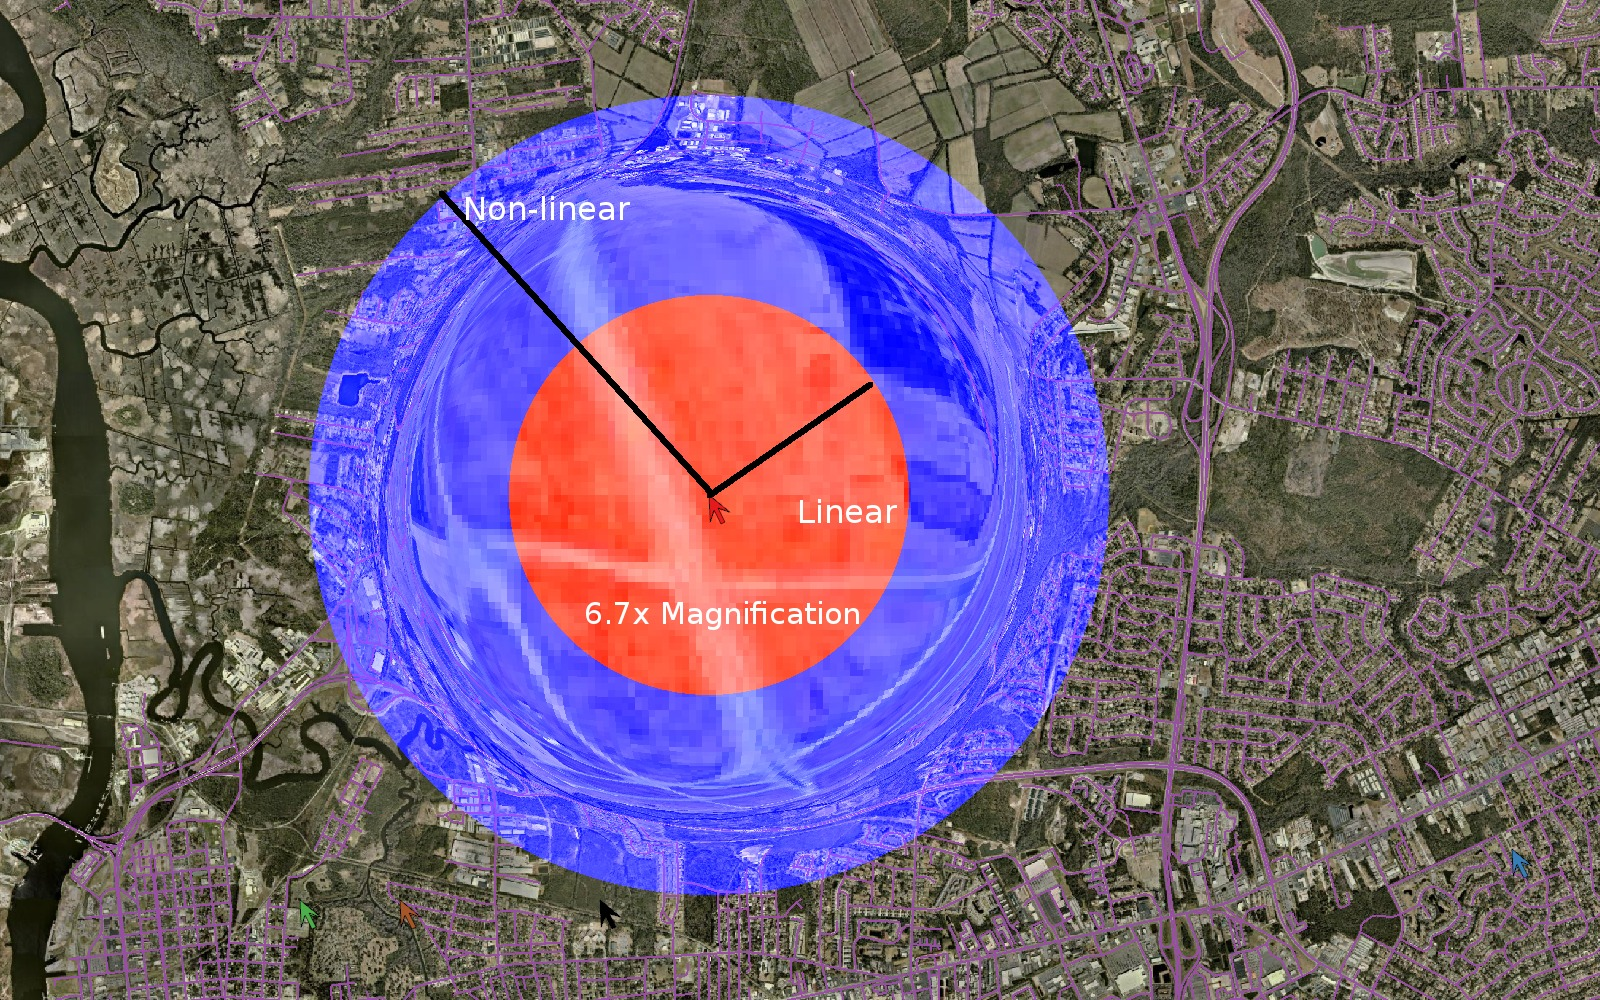
\includegraphics[width=0.8\linewidth]{img/regions_diagram.jpg}
    \caption[Combined Linear and Non-linear Magnification Regions]{An image of our infrastructure visualization magnification regions. The blue area is the non-linear magnification and the red region is the linear magnification. Note that despite being distorted, the roads in the image are still connected in both regions, allowing the user to trace a continuous path.}
    \label{fig:regions_diagram}
\end{figure}

Keahey and Robertson also note that performing such transformations on different domains has different requirements. When manipulating graph networks, the overall adjacency of nodes and edges is maintained for most transformations, linear or non-linear. Visual data requires more focus on the boundaries between the different transformation functions, as the boundary regions are especially susceptible to visual errors if they are not C0 continuous. An example image of a
magnification function that is not C0 continuous is seen in Figure~\ref{fig:non_continuous}. This resulting magnification includes a loss of data due to the discontinuity. These concerns are directly
applicable to designing a solution, as our data is stored in both a graph network and a series of satellite images. 

\begin{figure}[htp] \centering
    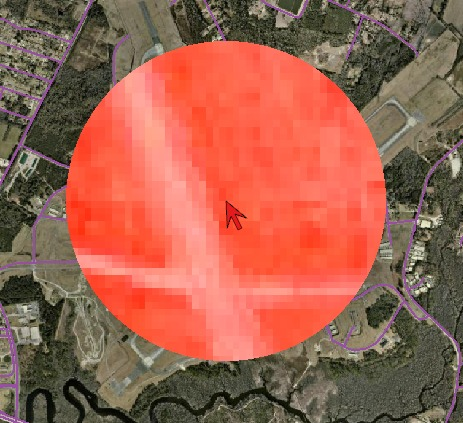
\includegraphics[width=0.3\linewidth]{img/non_continuous.jpg}
    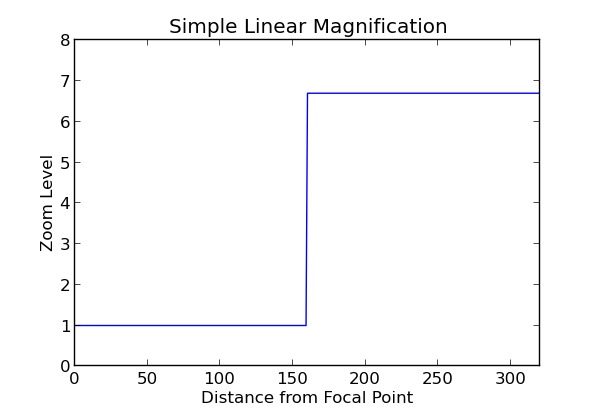
\includegraphics[width=0.6\linewidth]{img/discontinuity_graph.jpg}
    \caption[Loss of Visual Data]{The magnification function for this transformation is not C0 continuous, and as such, causes a loss of data and discontinuities of geographic data.}
    \label{fig:non_continuous}
\end{figure}

In addition to discussing the relevant concerns of combining transformation functions, Keahey and Robertson describe a few methods for combining regions of magnification. Of particular note is his proposal for weighted averaging that simply transforms a point by all nearby functions and calculates weights as the inverse of the distance between the center of magnification and the original point. This method does not obscure data, and is simple to implement for our purposes

In this new paper, Keahey and Robertson generalize the non-linear magnification problem by removing the concept of foci \cite{Keahey1997}. They make a distinction between transformation and magnification, where the former indicates the distortion of the space, with the magnification function being the derivative of the transformation function. By generalizing the problem to a scalar field, we can derive the magnification of a particular element based on its own properties. Given a particular magnification mesh, computing a corresponding transformation grid is difficult, as it involves trying to convert a single magnification value into a two coordinate system. The solution presented uses an iterative method to approximate a numerical solution. The work done in is well suited to the task at hand for our data when either the satellite images or graph network are displayed
independently. However, we still need to create our own magnification functions to modify the underlying scalar field and create a region of linear zoom. This method simply removes the need for thinking about the magnification problem with regards to focal points. 

Keahey later generalizes the overall focus plus context problem into a detail plus context problem \cite{Keahey1998}. Up to this point, most focus context systems create focus by enlarging specific regions while compressing other regions. This does not inherently produce more detail within this region, as it simply makes the existing data easier to distinguish. He proposes a few different methods of adding detail to such regions like displaying different view levels. By
showing different view levels, the amount of information displayed in a region changes, as the original non-linear transformation merely causes a change in terms of size and shape. He mentions that this process could be used for map based data, and this technique is definitely helpful for future work (Chapter~\ref{chapter:future_work}).

In contrast to the fisheye visualizations of data presented by Kadmon and Shlomi, Sarkar and Brown, and Keahey and Robertson,  Elmqvist et al.\ present a method for folding space to achieve a focus plus context view \cite{Kadmon1978} \cite{Sarkar1992} \cite{Keahey1996} \cite{Elmqvist2010}. The other techniques present a visualization that is visually similar to a fisheye lens, focusing more on having a lot of global data. This method contextually folds 2D data into 3D such that
the only regions displayed are areas within focus. This devotes most of the screen space to the focal points at the cost of being able to see most of the global data. Where other techniques that utilize focus plus context expand the region around focal points, the system
created by Elmqvist et al.\, M\'{e}lange, compresses the
unimportant areas of the display. A diagram of this system is seen in Figure~\ref{fig:melange}, notice that the red region, corresponding to the magnified areas, take up the majority of the display. Relative distance between focal points within the distorted region is represented by a number of folds, each indicating a complete screen distance. While this method produces interesting results, it is important in our visualization to have a majority of the information undistorted. M\'{e}lange focuses on showing as much detail around the focal points as possible, but the goals for a visualization of our system are to show a smaller area of increased focus while maintaining as much context as possible.

\begin{figure}[htp] \centering
    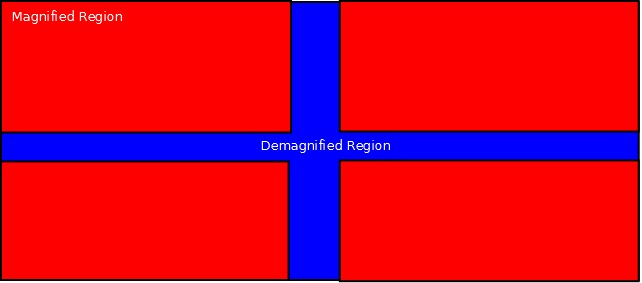
\includegraphics[width=0.45\linewidth]{img/Melange.jpg}
    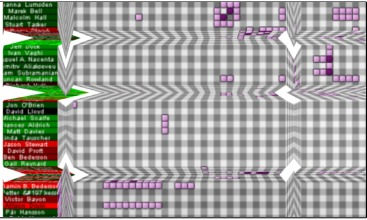
\includegraphics[width=0.45\linewidth]{img/melange_actual.jpg}
    \caption[M\'{e}lange Diagram]{An image comparing magnified and demagnified regions of the M\'{e}lange system 
    \cite{Elmqvist2010}, developed by Elmqvist et al.\ as well as the system applied to a visualization of an   
    adjacency diagram.}
    \label{fig:melange}
\end{figure}

B\"{o}ttger et al.\ present a method for manipulating a distorted city map to highlight specific areas of interest in \cite{Bottger2008}. The motivation for this system was the combination of geographic data and a stylized subway network to display more information around areas on the stylized network diagram. They introduce a concept called \emph{Warping Zoom}. Given a set of control points, they create a mapping function which moves any number of control points to other positions.
These individual control points correspond to the different subway stops and routes on the original mapping and are moved to positions to form the stylized network. While this method would allow for the separation of clustered data within our visualization by warping the overall data, it does not provide a solution for viewing the satellite data at a higher level of detail, nor does it perform an easily classifiable magnification function. To perform a magnification of a region of
satellite images, the system would have to define multiple control points and their resulting position. This is essentially performing the same transformation as a simple magnification function, but only focuses on manipulating a few points. 

\section{Summary}
\label{section:PREVIOUS_WORK_SUMMARY}

This chapter provided an overview of works which attempt to use a focus plus context visualization. I discussed a variety of applications which focused on utilizing some sort of focus plus context solution to solve their visualization issues. Finally, applications and research which concerned geometric distortions of data were summarized with respect to our goals. The following chapter discusses the changes performed to our visualization to improve performance and allow for implementation of our magnification function.


%%%%%%%%%%%%%%%%%%%%%%%%%%%%%%%%%%%%%%%%%%%%%%%%%%%%%%%%%%%%%%%%%%% 
%                                                                 %
%                           METHODS                               %
%                                                                 %
%%%%%%%%%%%%%%%%%%%%%%%%%%%%%%%%%%%%%%%%%%%%%%%%%%%%%%%%%%%%%%%%%%% 
 
% \specialhead{METHODS}
\chapter{VISUALIZATION}
\label{chapter:visualization}
As stated in Chapter~\ref{chapter:intro}, this thesis work started as a proof of concept for performing
real-time fisheye deformations on Graphics Processing Units(GPU) using OpenGL 3.1. The previous version of the visualization application used the OpenGL 2.0 specifications (referred to as legacy OpenGL from here on). OpenGL 3.0 specifications were released in September 2008, labeling many of the core functions as deprecated \cite{opengl_3_specification}. In Sections~\ref{section:legacy_opengl} and~\ref{section:modern_opengl}, a brief description of the relevant deprecated
functionality and the replacement methods is given. Section~\ref{section:base_mapview_elements} discusses the implementation details for upgrading the core functionality of the graph visualization. Finally, Section~\ref{section:satellite_images} and Section~\ref{section:road_network} details the rendering process of the satellite images and road network.

\section{Legacy OpenGL}
\label{section:legacy_opengl}

The standard for rendering polygons in legacy OpenGL was immediate mode. The functions {\tt glBegin()} 
and {\tt glEnd()} indicate that the calls to {\tt glVertex()} form a polygon specified by the call to {\tt glBegin().} 
All vertices specified this way can also have texture coordinates, colors, and normal vectors 
passed to OpenGL for rendering. These shapes are drawn immediately to the buffer after the 
call to {\tt glEnd().} Listing~\ref{lst:simple_triangle} shows a code sample for rendering a colored triangle in legacy OpenGL. 

\begin{lstlisting}[float, 
    caption={[Legacy OpenGL Colored Triangle] Rendering a triangle with a red, blue, and green corner.},
    label={lst:simple_triangle}]
glBegin(GL_TRIANGLES);
glColor3f( 1.0, 0.0, 0.0);
glVertex2f( 0.0, 1.0 );
glColor3f( 0.0, 1.0, 0.0):
glVertex2f( 1.0, -1.0 );
glColor3f( 0.0, 0.0, 1.0);
glVertex2f( -1.0, -1.0 );
glEnd()
\end{lstlisting}

Rendering in a 3D environment involves the transformation of vertex positions. First the coordinates 
are transformed from object space to world space, where object space has vertices defined relative 
to an object's center point and world space has vertices defined relative to all other objects 
within the world. Defining objects in world space places objects within the world, akin to placing props on a stage. The coordinates are then transformed to eye space, which represents their 
positions relative to the viewer. The viewer is assumed to be at the origin in world space, looking in the negative z direction. Eye space is useful for defining how far away any particular object is from the viewer, which is represented as the z direction.  Finally, eye space is transformed  to projection space, where objects are projected onto a 2D screen based on their positions and distance from the user. Each of the respective transformations are represented by different matrices. The model, view, and projection matrices correspond to the transformation to world, eye, and projection space, respectively \cite{opengl_matrix_stack}. 

In legacy OpenGL, these matrices were handled by a matrix stack ({\tt glPopMa\-trix(),} {\tt glPushMatrix()).} 
The model and view matrices were combined into a single matrix for OpenGL, represented by the 
constant {\tt GL\_MODELVIEW\@}. The projection matrix, {\tt GL\_PROJECTION}, was handled by either {\tt glOrtho()} 
or {\tt glFrustum()} for either an orthographic or standard projection.

Because we are rendering a 2D environment, we use an orthographic projection to ensure that 
objects are not scaled by the environment based on their distance away from the camera, this ensures that changing the level of detail of the overall system does not cause objects to become too small to perceive or to become too large to view anything else. An orthographic projection allows us to utilize the z dimension as a method of choosing the order in which elements should be displayed, i.e.\ which elements will be drawn over other elements within the overall application.

\section{Modern OpenGL}
\label{section:modern_opengl}

Our application uses OpenGL 3.2 specifically to use geometry shaders as part of our core functionality. Version 3.0 of OpenGL marked functions in legacy OpenGL as deprecated, but they were not officially removed from the core profile until OpenGL 3.1. To avoid further confusion between different versions, we will refer to OpenGL 3.2 as modern OpenGL.

Passing vertex data to OpenGL via the above method of {\tt glBegin()} and {\tt glEnd()} was deprecated for modern OpenGL\@. Rendering now requires the usage of vertex and fragment shaders, 
programs that run on the Graphics Processing Unit (GPU) and operate on vertices and the interpolated 
screen fragments surrounded by the vertices.  The previous methods for changing attributes of a particular vertex relied on the fixed function pipeline. This change was introduced due to the overall flexibility of shaders. While shaders are more expressive than the fixed function pipeline of legacy OpenGL, they require more code for simple tasks.

In a standard draw function using modern OpenGL, data is specified in Vertex Buffer Objects (VBOs) 
which contains the data that is sent to the vertex shader. VBOs are the GPU equivalent of Vertex Arrays, batches of vertex data stored in CPU address space. Vertex Arrays were deprecated as their performance when compared with VBOs were much worse due to requiring data to be transfer ed to the GPU on every frame. VBOs provide a mechanism for utilizing GPU memory within OpenGL~\cite{opengl_3_specification}. VBOs contain the same data that 
would be called between the {\tt glBegin()} and {\tt glEnd()} calls, and are created and activated with 
the {\tt glGenBuffers()} and {\tt glBindBuffer()} commands. The function {\tt glBufferData()} allocates memory for the data on the GPU and is given a pointer to sequential memory that will be copied into the GPU\@. Different VBOs or regions of memory are then referred to by vertex attribute pointers using the {\tt glVertexAttribPointer()} function. These pointers inform the vertex shaders how to interpret the data. If necessary, any extra data can be passed to the vertex and fragment shaders via calls to {\tt glUniform()}. The two commands, {\tt glDrawArrays()} and {\tt glDrawElements()}, are used to specify a range of data to be drawn by OpenGL, sending data as necessary.

Listing~\ref{lst:modern_triangle} shows a C++ code sample of specifying the same triangle in Listing~\ref{lst:simple_triangle} with modern OpenGL\@. Listing~\ref{lst:vertex_shader} and~\ref{lst:fragment_shader} show the necessary vertex and fragment shaders, respectively.

\lstinputlisting[ caption={[Modern OpenGL C++ Colored Triangle]Rendering a triangle with a red, blue, and green 
    corner. The C++ code generates the necessary VBO, one for position and one for color, inserts the data, and 
    then renders the triangle.},
    label={lst:modern_triangle}]
{data/modern_triangle.cpp}

\lstinputlisting[ caption={[Colored Triangle Vertex Shader]The vertex shader for {\tt triangleProgram}. The 
    shader receives the position and color data and passes this information to the fragment shader through the 
    out variable.},
    label={lst:vertex_shader}]
{data/simple.vert}

\lstinputlisting[ caption={[Colored Triangle Fragment Shader]The fragment shader for {\tt triangleProgram}. The 
    shader receives the interpolated color and position from the vertex shader and outputs data to the screen.},   
    label={lst:fragment_shader}]
{data/simple.frag}

Functionality related to the matrix stack was also deprecated for modern OpenGL\@. Developers must now manage their own matrices and vectors. This was another side effect of removing the fixed function pipeline. Much like the addition of shaders, the modern OpenGL specification made this change to allow for greater flexibility. Developers do not have to conform to using the {\tt GL\_MODELVIEW} and {\tt GL\_PROJECTION} matrices for their transformations. The GLM library
\cite{glm_website} was developed to duplicate this missing functionality and act as a CPU implementation of the OpenGL Shader Language (GLSL) vector and matrix operations. These matrices and other variables are passed to the shaders as uniform variables (variables that are constant across all invocations of a shader). The vertex shader is now responsible for performing any relevant operations on a per-vertex basis. These operations include transforming a vertex's position in model or
world space to projection space and light calculations based on a vertex's normal vector. After this step, coordinates are expected to be in Normalized Device Coordinates (NDC), which range from -1 to 1 in the x, y, and z directions. The area between a triangle is then broken into different fragments. Any data that was stored in the three vertices is interpolated over this entire region. Each of these fragments is operated on by the fragment shader. The fragment shader is
responsible for choosing the resulting color of a particular fragment before the scene is rendered to the display.

While vertex and fragment shaders are mandatory due to their equivalent functionality being removed from the fixed function pipeline, geometry shaders provide an optional method of manipulating vertex data on the GPU\@. Given input data in the form of points, lines, or triangles, the geometry shader is able to modify vertex data between the vertex and fragment shaders. Figure~\ref{fig:shader_pipeline} shows the OpenGL shader pipeline for the infrastructure visualization.

\begin{figure}[htp] \centering
    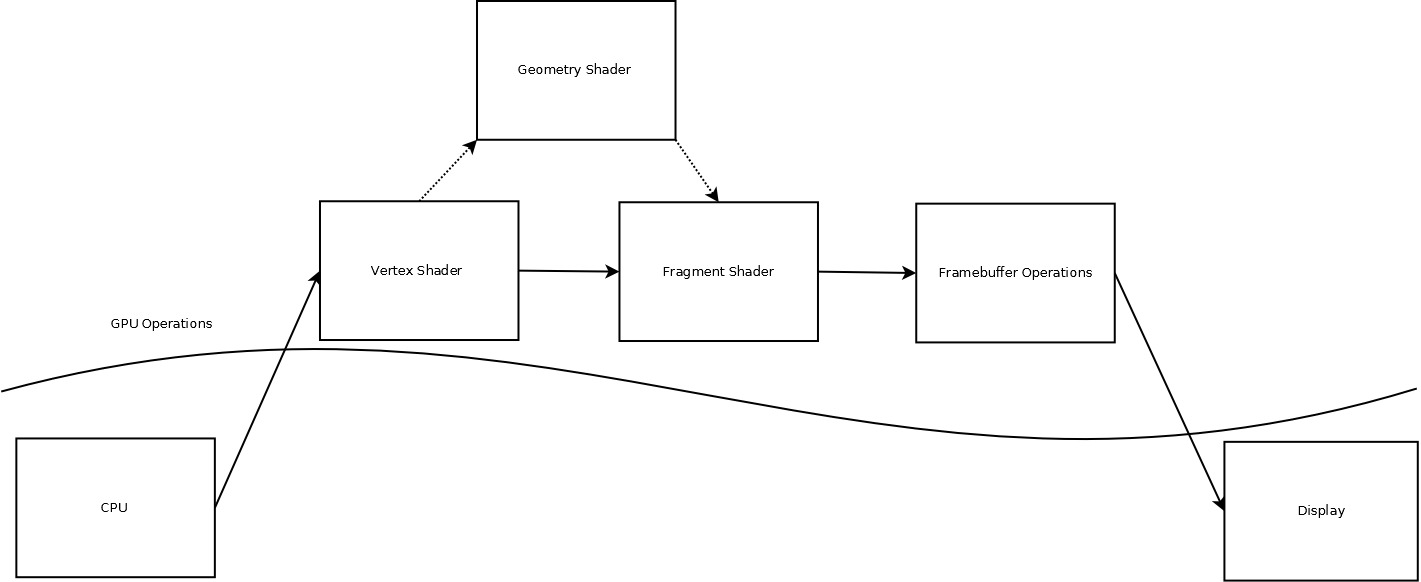
\includegraphics[width=150mm]{img/pipeline.jpg}
    \caption[Infrastructure Visualization Shader Pipeline]{An overview of the visualization's shader pipeline.}
    \label{fig:shader_pipeline}
\end{figure}

\section{Base Visualization Elements}
\label{section:base_mapview_elements}

The following sections, describe the rendering methods of different base elements that are used in different places throughout the entire application. Each section explains the usage of individual elements, describes the method used in the previous versions of the visualization for rendering, and is concluded by the method used for modern OpenGL compliance.

\subsection{Buttons}
\label{subsection:buttons}
For the visualization, buttons are the nodes of the graph network. Their default state is a circle such that all nodes of a particular resource are colored the same. When expanded, these elements increase in area and take on the shape of squares. These squares are then overlaid by text describing relevant status information. This visual change is to allow users to easily pick out nodes which have more information, as well as to allow for more space for text to be drawn. Every button has at least one associated border
with it in an attempt to provide further distinction between nearby nodes. Multiple borders surrounding a node indicates that a node is not receiving the resource associated with the color. Figure~\ref{fig:buttons} shows two nodes, one expanded and the other unexpanded.

\begin{figure}[htp] \centering
    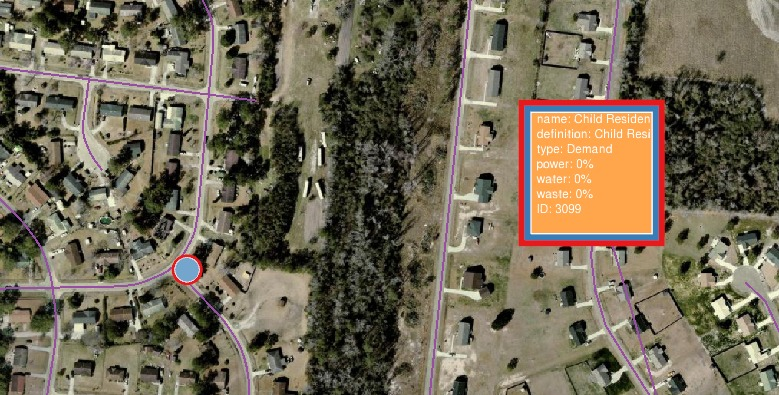
\includegraphics[width=0.8\linewidth]{img/buttons.jpg}
    \caption[Buttons]{An image showing two nodes of the graph network. The expanded node has a significantly greater area than the unexpanded node. Both nodes have a red border, indicating a lack of power. The expanded node has a lack of water as well, shown by the blue border.}
    \label{fig:buttons}
\end{figure}

The implementation of drawing buttons in the legacy OpenGL code followed the format of the 
pseudocode seen in Algorithm~\ref{alg:button_drawing}.

\begin{algorithm}
    \caption{Pseudocode detailing the general process of rendering a button in the legacy OpenGL
    version of the visualization.}\label{alg:button_drawing}
    \begin{algorithmic}[1]
        \Function{Button Drawing}{}
            \ForAll{Button in Buttons}
                \If{Button is not expanded}
                \State\Call{DrawCircleBorder}{Button}
                    \If{Button is textured}
                        \State\Call{DrawCircleTexturedButton}{Button}
                    \Else
                        \State\Call{DrawCircleUntexturedButton}{Button}
                    \EndIf
                \Else
                    \State\Call{DrawRectangleBorder}{Button}
                    \If{Button is textured}
                        \State\Call{DrawRectangleTexturedButton}{Button}
                    \Else
                        \State\Call{DrawRectangleUntexturedButton}{Button}
                    \EndIf
                    \If{Button has text}
                        \State\Call{DrawText}{Button}
                    \EndIf
                \EndIf
            \EndFor
        \EndFunction
    \end{algorithmic}
\end{algorithm}

The borders representing state data are drawn first, followed by either an untextured or textured 
main button area. Finally, if a button is expanded and has corresponding text, the text is 
also drawn. A button and all of its related elements (text and borders) are given the same z value when rendered. This z value is the ``depth'' of the element within the overall scene relative to the camera, such that elements with a lower z value are closer to the camera, and elements with a higher z value are further away. Because we are using an orthographic projection, this information allows us to choose the order in which we render objects.OpenGL provides methods for determining if a
new pixel should be drawn based on the information in the depth buffer. A call to {\tt glDepthFunc(GL\_LEQUAL)} tells OpenGL that the current pixel in a location should be discarded if the new pixel has a z value less than or equal to the current amount stored in the depth buffer \cite{opengl_depth_buffer}. This method of The drawing order is important to note, as elements with the same z order will be drawn in the order that calls to {\tt glDrawArrays()} are performed, this is known
as the Painter's algorithm \cite{Berg1993}. In the previous version of OpenGL, the entirety of the layering was handled by Painter's algorithm, requiring all of the buttons in the application to be sorted every frame. Figure~\ref{fig:layering_buttons} shows the layering of buttons.

\begin{figure}[htp] \centering
    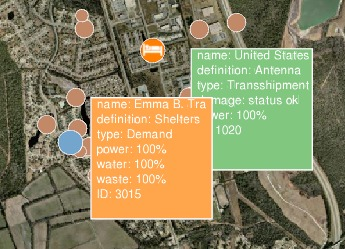
\includegraphics[width=0.8\linewidth]{img/button_layering.jpg}
    \caption[Button Layering]{Elements that have been interacted with have a lower z value and are drawn over other buttons. Text has the same z value as the underlying button, but is drawn later, so is still visible on the expanded.}
    \label{fig:layering_buttons}
\end{figure}

The drawing of buttons and their borders relied on two drawing formats in legacy OpenGL that were 
completely removed in OpenGL 3.1, {\tt GL\_QUADS} and {\tt GL\_POLYGON\@}. Duplicating the {\tt GL\_QUADS} functionality 
is trivial with {\tt GL\_TRIANGLES} or {\tt GL\_TRIANGLE\_STRIP\@}. For a quadrilateral with vertices a, b, 
c, d, create one triangle with vertices a, b, c and one with vertices a, c, d. We elected to 
use {\tt GL\_TRIANGLES}, as {\tt GL\_TRIANGLE\_STRIP} indicates that the entire range of vertices passed to
{\tt glDrawArrays()} is a continuous strip of triangles, and would necessitate multiple function 
calls to draw multiple rectangular buttons.

{\tt GL\_POLYGON} allowed a user to specify a convex polygon with $N$ sides. This was used to create 
a 20-sided polygon to approximate the appearance of a circle. Every adjacent pair of vertices 
specified forms one edge, with vertices 1 and $N$ forming the last edge of the polygon. There are a few choices for replicating {\tt GL\_POLYGON} functionality. {\tt GL\_TRIANGLE\_FAN} best approximates 
the old functionality by taking a center vertex and forming individual triangles out of every 
adjacent pair of vertices and the center vertex. Using {\tt GL\_TRIANGLE\_FAN} reduces the number of vertices that have to be specified to draw a circle. Unfortunately, this approach has the same 
downside that using {\tt GL\_TRIANGLE\_STRIP} for drawing rectangular buttons has, drawing $N$ circles 
with this method requires $N$ calls to {\tt glDrawArrays()}, as all vertices in the range passed to {\tt glDrawArrays()} are considered to be connected to the first vertex specified. Much like drawing rectangular buttons, using {\tt GL\_TRIANGLES}
allows for all of the circular buttons to be drawn in one call to {\tt glDrawArrays().}

Replacing the old functionality was considered, but the individual buttons never stored the 
vertex data for {\tt GL\_POLYGON}, it was simply computed as needed based on a center point, and a 
radius. Instead of calculating these new triangles on every frame on the CPU, we chose to use a geometry 
shader, which performs the same operations but specifies 59 less vertices and can be computed in parallel. To generate a circular button, the geometry shader constructs 20 triangles with the 
following algorithm (Algorithm~\ref{alg:circle_geometry}). 

\begin{algorithm}
    \caption{Creating a circle from 20 individual triangles given a center point and a radius. This can be implemented on the CPU or the GPU.}
    \label{alg:circle_geometry}
    \begin{algorithmic}[1]
        \Function{CreateCircle}{$\vec{center}$, $radius$}
        \For{$i=0 \rightarrow 20$}
            \State $a_0 = \frac{2\pi(i \% 20 )}{20}$ 
            \State $a_1 = \frac{2\pi((i+1) \% 20 )}{20}$ 

            \State $\vec{p_0} = \vec{center} + radius \times \langle cos(a_0), sin(a_0) \rangle$
            \State \Call{createVertex}{$\vec{p_0}$}

            \State \Call{createVertex}{$\vec{center}$}

            \State $\vec{p_1} = \vec{center} + radius \times \langle cos(a_1), sin(a_1) \rangle$
            \State \Call{createVertex}{$\vec{p_1}$}
        \EndFor
        \EndFunction
    \end{algorithmic}
\end{algorithm}

This algorithm replicates the functionality performed in the previous version of the visualization by 
generating triangles that have the center vertex and two vertices that are created by taking 
20 uniform samples of the circle expressed by the center vertex and the radius.

We use a total of four VBOs when rendering the buttons: Untextured circular buttons and circular borders,
Textured circular buttons, untextured rectangular buttons and rectangle borders, and textured rectangle 
buttons. The different types of buttons except the textured rectangle, as it is not currently used within the system, can be seen below.

The data in the VBOs change depending on the status of the button. If the underlying data representation changes, then the text of a button and its borders may change. When a button expands or contracts, data must be placed in different VBOs.

\begin{figure}[htp] \centering
    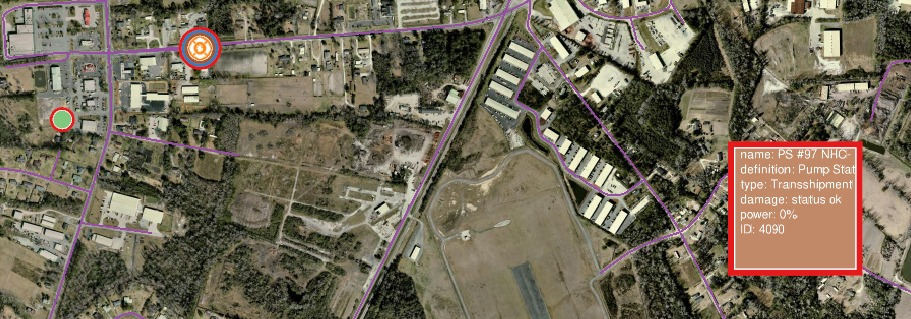
\includegraphics[width=0.8\linewidth]{img/button_types.jpg}
    \caption[Button Types]{An image showing the three types of buttons used within the visualization. From left to right, we see a untextured circular button, a textured circular button, and a untextured rectangle. The nodes are surrounded by colored borders that indicate problems with the supplied services. The button on the lower right is lacking power, hence the red border. The main button color indicates the service type, in this case brown represents the waste/sewage network. }
    \label{fig:button_types}
\end{figure}

\subsection{Lines}
\label{subsection:lines}

Drawing lines in modern OpenGL functions the same as drawing in legacy OpenGL with two major caveats. 
Legacy OpenGL allowed for calls to {\tt glLineWidth()} to set the integer width of drawn lines to a specific 
screen space value. This feature has been deprecated in OpenGL 3.1, resulting in the inability to 
have lines with a width greater than 1.0. Lines must also be passed into VBOs and rendered by a vertex and fragment shader.

To solve the line width problem, we utilize a geometry shader to create two triangles that form a quadrilateral 
that has a pixel width based on an input value. Pseudocode for the geometry shader is shown 
in Algorithm~\ref{alg:line_geometry}. In essence, the two endpoints of a line segment are pushed apart by half 
of the total width of the resulting line, generating four points total.

\begin{algorithm}
    \caption{Creating a rectangle from two triangles given the end points of a line segment and a width.}
    \label{alg:line_geometry}
    \begin{algorithmic}[1]
        \Function{CreateRectangle}{$\vec{p_0}$, $\vec{p_1}$, $width$}
        \State $dx = p_{1x} - p_{0x}$
        \State $dy = p_{1y} - p_{0y}$

        \State $\vec{normal} = \langle -dy \times \frac{width}{2}, dx \times \frac{width}{2}\rangle$
        \State $\vec{p_{00}} = \vec{p_0} + normal$
        \State $\vec{p_{01}} = \vec{p_0} - normal$

        \State $\vec{p_{10}} = \vec{p_1} + normal$
        \State $\vec{p_{11}} = \vec{p_1} - normal$

        \State \Call{createVertex}{$\vec{p_{00}}$}
        \State \Call{createVertex}{$\vec{p_{01}}$}
        \State \Call{createVertex}{$\vec{p_{10}}$}
        \State \Call{createVertex}{$\vec{p_{11}}$}

        \EndFunction
    \end{algorithmic}
\end{algorithm}

Drawing continuous lines with this method results in seeing disjoint areas where lines connect. 
To solve this graphical issue, we draw a circle at each endpoint with a radius equal to the width of the expanded line on the GPU using Algorithm~\ref{alg:circle_geometry}. Figure~\ref{fig:line_no_joint} shows a line segment without the circles drawn on the endpoints, and Figure~\ref{fig:line_joint} shows the same line segment with circular endpoints 

\begin{figure}[htp]
    \centering
    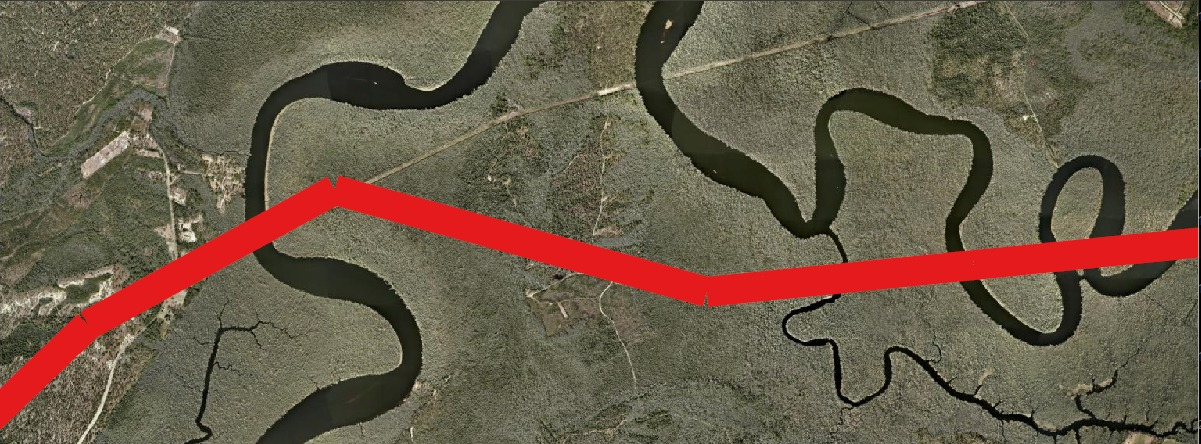
\includegraphics[width=0.90\linewidth]{img/expanded_edge_no_joint.jpg}
    \caption[Line Segment without Joints Drawn]{A line drawn by expanding multiple a line segments into rectangles. The individual segments are clearly visible due to the construction method.}
    \label{fig:line_no_joint}
\end{figure}
\begin{figure}[htp]
    \centering
    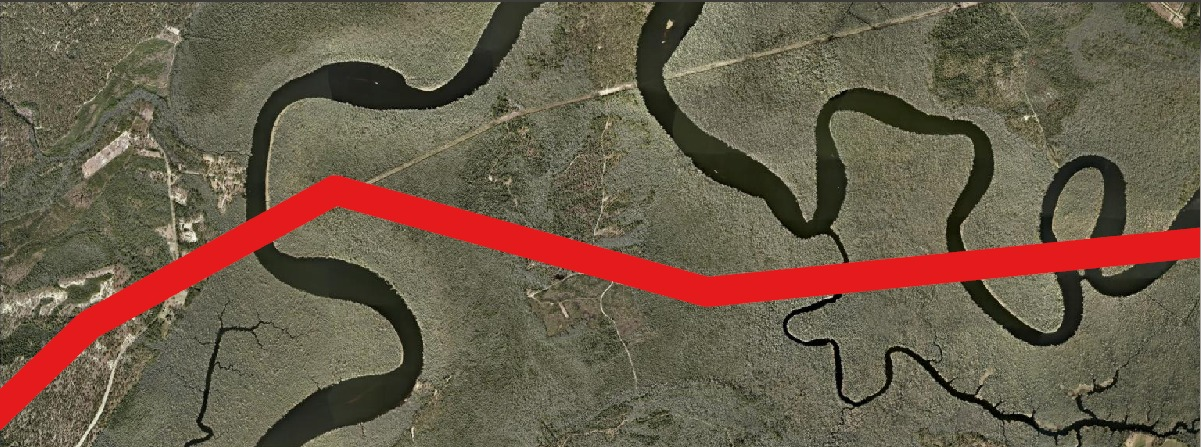
\includegraphics[width=0.90\linewidth]{img/expanded_edge_joint.jpg}
    \caption[Line Segments with Joints Drawn]{The same line as the Figure~\ref{fig:line_no_joint} but with circular joints drawn on the endpoints for the segments.}
    \label{fig:line_joint}
\end{figure}

The width of each line segment changes depending on if the overall graph edge in the network is expanded or not. These expanded lines have text drawn on them, displaying information about the status of transmitting a resource between the two nodes it connects. This status string is fairly short, and is therefore repeated over the entire length of the edge to ensure that the edge information is conveyed to the user. The figure below shows an example of an unexpanded line and an expanded line.

The previous version of the visualization used {\tt GL\_LINE\_STRIP} to draw individual line segments with only 
N vertices to represent a line with $N-1$ segments. Much like the issues discussed with rendering 
many buttons with {\tt GL\_TRIANGLE\_STRIP} in Section~\ref{subsection:buttons}, if individual lines continue to 
use the  {\tt GL\_LINE\_STRIP} format, $N$ calls to {\tt glDrawArrays()} are needed to draw $N$ different lines. While we do not have concrete timed data, the old method of rendering caused noticeable lag if the main source of lines, the road network, was being rendered. This lag would disappear if the road network was turned off. To sidestep 
this problem, we create individual line segments out of each of the specified line strips. 
While this construction roughly doubles the number of vertices for each line, the overall benefits 
in terms of code simplicity and performance make it a worthwhile change.

We use a total of two VBOs for rendering all of the lines in the program, one for the line segments,
and another for the endpoints. The depth buffer handles the layering of the lines, similar to the buttons, this prevents sorting every edge of the application every frame. Similarly to buttons, lines must have their data reloaded whenever the underlying data changes or the edge expands or contracts. 

\subsection{Text}
\label{subsection:text}

Rendering text is a major technical challenge when using a low level library such as OpenGL\@. 
Prior to the upgrade, the visualization used a third-party library, The OpenGL Utility Toolkit (GLUT), 
\cite{glut_website} for handling text and mouse and keyboard events. The changes required in the rest of the application also necessitated the removal of GLUT, as it was dependent on the matrix 
stack to perform its rendering.

GLUT utilized multiple line segments to draw the different characters and provided utility functions
to query the width and height of the resulting characters.

We solve the basic problem of rendering text by using the FreeType font library 
\cite{freetype_website}. A specific font is loaded by the visualization during its initialization. 
Every character is a bitmap with values from 0 - 255. All of the relevant ASCII 
characters are loaded into a single 2D texture. To render any arbitrary block of text, 
a quadrilateral is generated from two triangles that has the dimensions of the current 
character. When the texture is applied to the colored triangles, the bitmap is sampled 
as the alpha channel, resulting in only the character being visible on screen. A generated font atlas is shown below in Figure~\ref{fig:font_atlas}.

\begin{figure}[htp] \centering
    
\includegraphics[width=1.0\linewidth]{img/font_atlas.jpg}
    \caption[Font Atlas]{A generated font atlas for usage in our application using the FreeSans TrueType font.}
    \label{fig:font_atlas}
\end{figure}


While buttons and paths are defined with respect to world space, it is much easier conceptually
to position buttons in terms of window coordinates. Text placement and manipulation is preferable 
when positioned in screen space, as text sizes are defined in terms of fractional pixels.
To achieve this, we transform the button coordinates into projection space. The range for values 
on the screen when performing the transformation this way is $-1.0$ to $1.0$. This range is then converted to 
values between 0 and the screen width in pixels for the x axis and 0 and the screen height for the y axis. 

Rendering lines of text for buttons is fairly simple. The data stored by the application is 
already stored as individual lines, Each line is drawn individually, and any characters that 
would leave the inner button region are simply not drawn.

When drawing text on an edge, a specific string of text is simply repeated for the entire length of the path, as mentioned in Section~\ref{subsection:lines}. To create this text, for every two adjacent vertices on a path, the distance between them is calculated. This distance is the upper limit for the amount of text that can be displayed on that particular line segment. An algorithm detailing the above process is seen below (Algorithm~\ref{alg:path_text}).

\begin{algorithm}
    \caption{A function for repeating a string across multiple line segments. $segments$ is an array of
    line segments, each segment having two points. $text$ is a string. The function returns an array of
    strings.}
    \label{alg:path_text}
    \begin{algorithmic}[1]
        \Function{PathText}{$segments$, $text$}
            \State $pos = 0$
            \State $results = []$
            \For{Every segment $s$ in $segments$}
                \State $pathText = ``''$
                \State $distance = |\vec{s_1} - \vec{s_2}|$
                \While{Total line width is less than distance }
                    \State Append $text[pos]$ to $pathText$
                    \State $pos = pos + 1$
                \EndWhile
                \State Append $pathText$ to $results$
            \EndFor 
            \State \Return{$results$ }
        \EndFunction
    \end{algorithmic}
\end{algorithm}

\begin{figure}[htp] \centering
    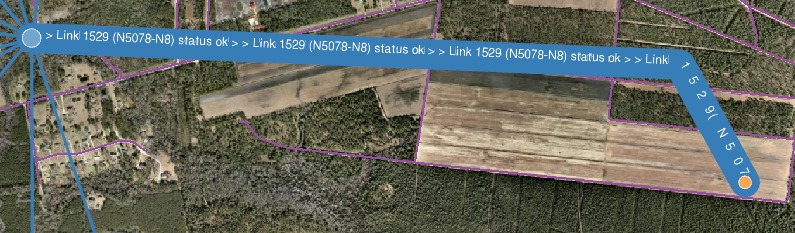
\includegraphics[width=0.8\linewidth]{img/text_path.jpg}
    \caption[Text Drawn on a Path]{An image showing text drawn on an expanded path. The string {\tt ``Link 1529 (N5078-N8) status OK > >''} is repeated over entire length of the path.}
    \label{fig:text_path}
\end{figure}

The individual triangles are then rendered after having the following transformation applied to the positions to line the text up with the path. Each vertex must be translated to the origin by the starting vertex's position, rotated by the calculated amount, and then translated back to original position due to the nature of rotations in OpenGL\@. 

We only need a single VBO for rendering all of the text for the application, even with rotated 
groups of text as described above.

\section{Satellite Images}
\label{section:satellite_images}

The satellite image layer of the visualization handles drawing satellite images at a given level of detail. 
This code required relatively few changes, as the main operations performed when rendering 
these images are independent of OpenGL calls. Andrew Zonenberg previously implemented a tile cache which loads different textures into RAM based on the current level of detail and camera position of the system. At most 10 images are fetched by the CPU and loaded as textures to draw any combination of satellite images for a particular scene. Each of these tiles is drawn as a quadrilateral made up of two triangles. A basic vertex and fragment shader render the textures.

In order to facilitate magnifying the satellite images, we render them to a Frame Buffer 
Object (FBO). FBOs allow for rendering data without immediately drawing this data to the screen. The satellite images are drawn to a texture that is same size as the screen. To render this final texture, we simply draw a quadrilateral that encompasses the entire screen, using the texture created by the FBO\@. 
This final texture does not need a model-view matrix, as we simply define it in terms of projection 
space.

\section{Road Network}
\label{section:road_network}

The previous implementation of rendering the roads in the visualization used an intermediate 
version of {\tt glDrawArrays()} which allowed CPU arrays to be bound as data (Vertex Arrays) to avoid using {\tt glBegin()} and {\tt glEnd()}. The road network was represented as an array of line strips, such that an individual road was either a single line segment for straight roads or multiple line segments for curved roads.

\begin{figure}[htp] \centering
    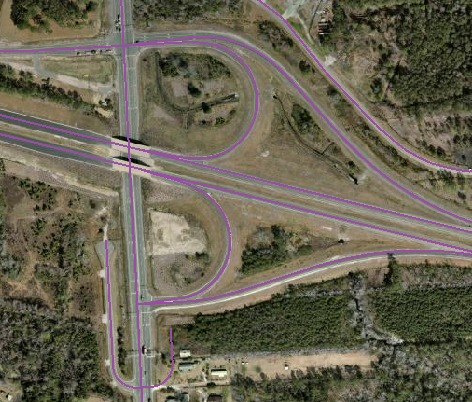
\includegraphics[width=0.8\linewidth]{img/satellite_and_road.jpg}
    \caption[Satellite Images and Roads]{An image showing a curved road, rendered with purple lines, on top of the satellite images.}
    \label{fig:satellite_and_road}
\end{figure}

An initial implementation of changing the rendering of the road network used {\tt glDrawArrays()} with 
these individual line strips. Each individual line strip was bound to a frame buffer and then 
immediately drawn. This rendering method had a negative impact on the overall performance of 
the application, as every invocation of {\tt glBufferData()} requires new data to be allocated. 

To solve the performance issues, the road network was transitioned to the method of rendering 
lines described earlier. All of the line strips are split into individual 
line segments  and stored in a single VBO\@. This new method of rendering allows for a single call to 
{\tt glDrawArrays().} This data is also static for the entire life of the the visualization, so we can improve 
performance even further by only loading the data into the VBO one time and using {\tt GL\_STATIC\_DRAW} 
to notify OpenGL that the data will not be changed after being initialized. The positioning of the road 
network is dependent on the model view projection matrices, and still requires the matrices 
to be passed in as uniform variables to be rendered correctly.

Similar to the satellite images, we render the road network to the FBO to allow the magnification 
to affect the road network.

\section{Summary}
\label{section:methods_summary}

This chapter discussed the changes to the code that were required for our magnification functions to be applied. A brief overview of the changes between legacy OpenGL and modern OpenGL were discussed, followed by the specific changes to the rendering system. The following chapter describes the non-linear magnification function used by our application and its implementation within our systems.

\chapter{MAGNIFICATION}
\label{chapter:magnification}
This chapter details the main contribution of this thesis work: the magnification effect generated by manipulating the distances for both the texture and the graph network. Subsection~\ref{section:texture_magnification} explains the process used in transforming the rendered FBO texture that the satellite images (Section~\ref{section:satellite_images}) and road network (Section~\ref{section:road_network}) both render to.

The requirements for this non-linear magnification of a texture include the ability to specify an inner and 
outer radius of magnification as well as a linear zoom factor. The program is intended to create a visual
effect such that the non-linear region between the inner and outer radii smoothly blends the regions of linear
zoom and base level magnification. The resulting function that accomplishes these goals should be easily
extensible to allow for multiple cursors interacting with the system at the same time. 

In performing magnification, we attempt to show more information to the users while ensuring that the data is still continuous. Some data loss will occur as regions become demagnified, but we attempt to minimize this as much as possible. As noted by Keahey and Robertson, our piecewise function should be continuous on its boundaries: the linear and non-linear functions should return the same value at the inner radius, and the non-linear function should return the input
value at the outer radius \cite{Keahey1996}.

A similar transformation is applied to the nodes and endpoints of line segments for the graph network. As mentioned previously in Chapter~\ref{chapter:intro}, most of the data in the graph network corresponds to
physical locations, so when the underlying satellite images get transformed by the texture magnification, the 
nodes and line segments must move accordingly. This process is explained in 
Subsection~\ref{section:graph_magnification}.

\section{Texture Magnification}
\label{section:texture_magnification}

To simulate magnification when dealing with rendering textures, we perform transformations the entire FBO texture
based on proximity to mouse cursors. Given three values, an inner radius, \emph{$r_0$}, an outer radius, 
\emph{$r_1$}, \emph{z}, a linear zoom factor, we construct two different formula for performing either a linear 
or non-linear magnification.

\begin{figure}[htp] \centering
    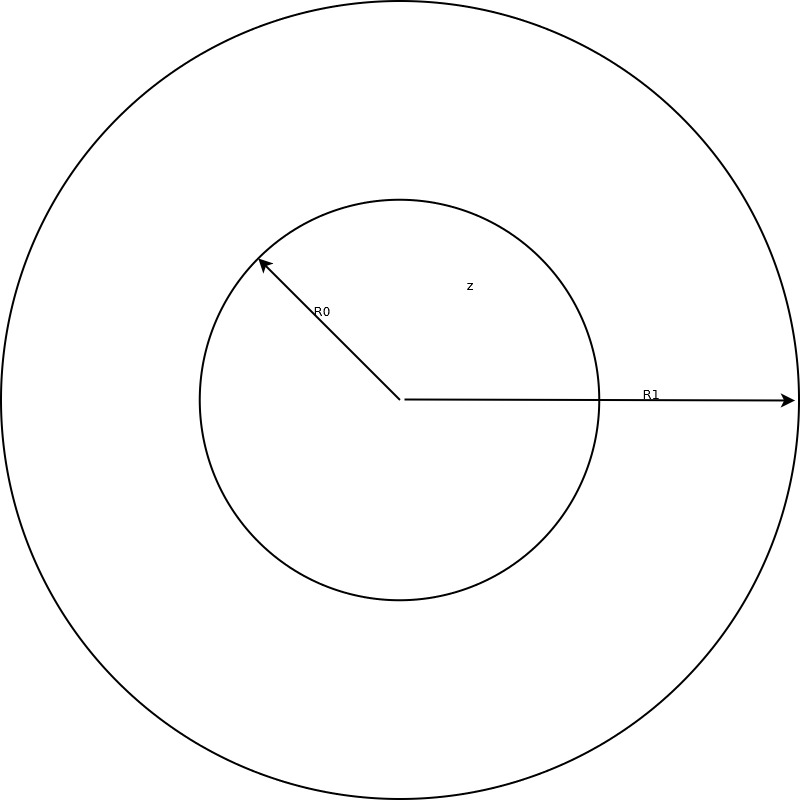
\includegraphics[width=0.4\linewidth]{img/cursor_mag.jpg}
    \caption[Magnification Parameters]{Visualization of the magnification parameters. \emph{z} is the linear zoom factor, \emph{$r_1$} is the outer radius, and \emph{$r_0$} is the inner radius.}
    \label{fig:mag_parameters}
\end{figure}

In both types of magnification, given the distance, \emph{d}, from a particular mouse cursor, $\vec{c}$,  to the 
original UV coordinate for a particular fragment, $\vec{p}$, the equations return a new scaled distance. This new 
distance, $f(d)$ is multiplied by the normalized direction vector between the mouse cursor, seen in
Equation~\ref{eq:magnifying_vector}.

\begin{equation}
    \label{eq:magnifying_vector} 
    v_i = f(d) \times \frac{\vec{c_i} - \vec{p}}{|\vec{c_i} - \vec{p}|}
\end{equation}

For distances less than \emph{$r_0$}, we perform linear magnification. The equation for which is given in 
Equation~\ref{eq:linear_magnification}

\begin{equation}
    \label{eq:linear_magnification}
    f(d) = d \times \frac{1}{z}
\end{equation}

We scale the distance by $\frac{1}{z}$ due to how UV sampling is performed. Reducing the area of the sampled 
texture spreads less information over the same area, resulting in the ability to see more data. An example of this is shown in Figure~\ref{fig:UV_sampling}.

\begin{figure}[htp] \centering
    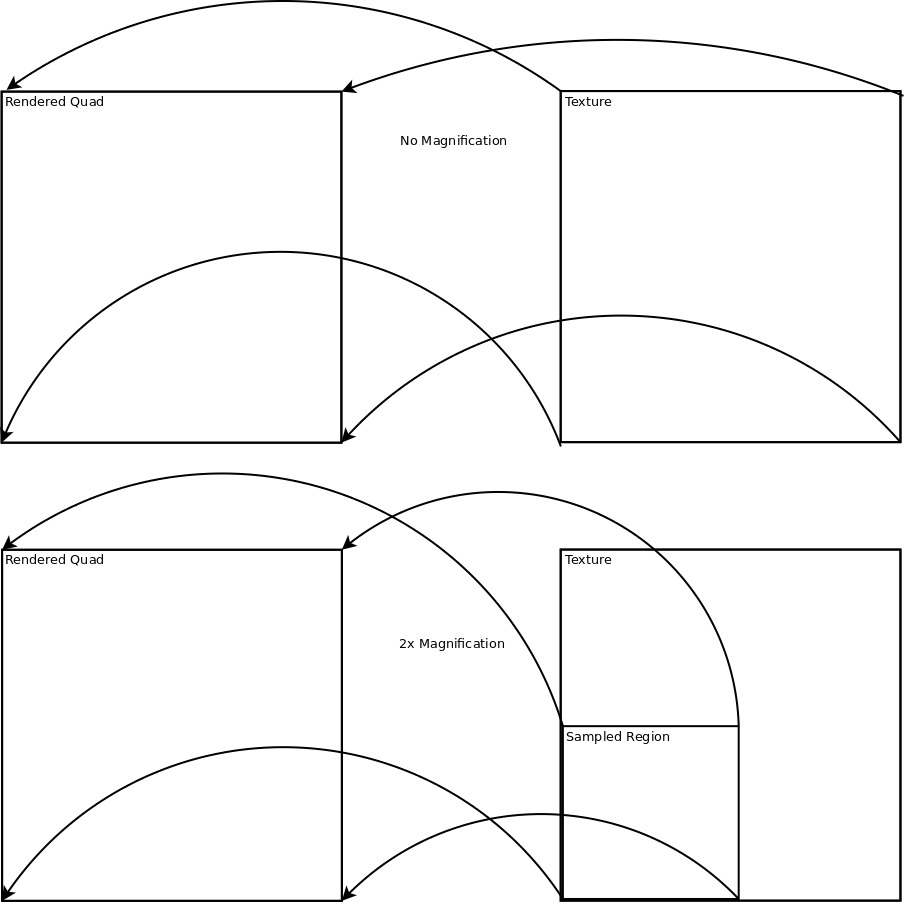
\includegraphics[width=0.6\linewidth]{img/texture_mag.jpg}
    \caption[UV Sampling]{Simple UV sampling example demonstrating magnification. The texture remains the same, we simply sample from a smaller region when performing magnification.}
    \label{fig:UV_sampling}
\end{figure}

For distances less than \emph{$r_1$}, we use the same premise of Equation~\ref{eq:linear_magnification}, but 
scale the linear zoom factor based on the distance away from the center instead of using a fixed value. To 
achieve this goal of a smooth, continuous image, we need a function which is continuous and has a smooth derivative. There are a few functions which follow the general form of having upper and lower limits; functions with a sigmoidal shape fall into this category. For our purposes, the desirable features are a smooth but rapid decrease from the higher magnification level, \emph{z} to the baseline level, 1. 
The generalized logistic function (Equation~\ref{eq:logistic_function}) fits these requirements as seen in 
Figure~\ref{fig:logistic_graph}, and is modified to fit our parameters, shown in 
Equation~\ref{eq:modified_logistic}

\begin{equation}
    \label{eq:logistic_function}
    f(x) = \frac{1}{1 + ae^{-bx}}
\end{equation}

\begin{equation}
    \label{eq:modified_logistic}
    f(d) = d \times \left( 1 + \epsilon + \frac{(z - 1 + 2\epsilon)}{1 + ae^{b(d-r_0)}}\right)
\end{equation}

The variables, \emph{a} and \emph{b}, can be solved for with the following two equations,~\ref{eq:solve_a} and~\ref{eq:solve_b}, essentially using a known given point to solve for the two variables.

\begin{equation}
    \label{eq:solve_a}
    a = \frac{\epsilon}{z - 1 + \epsilon}
\end{equation}

\begin{equation}
    \label{eq:solve_b}
    b = \frac{ln\left( \frac{\frac{z - 1 + 2 \epsilon }{\epsilon} + 1}{a}\right) }{r_1 - r_0}
\end{equation}

\begin{figure}[htp] \centering
    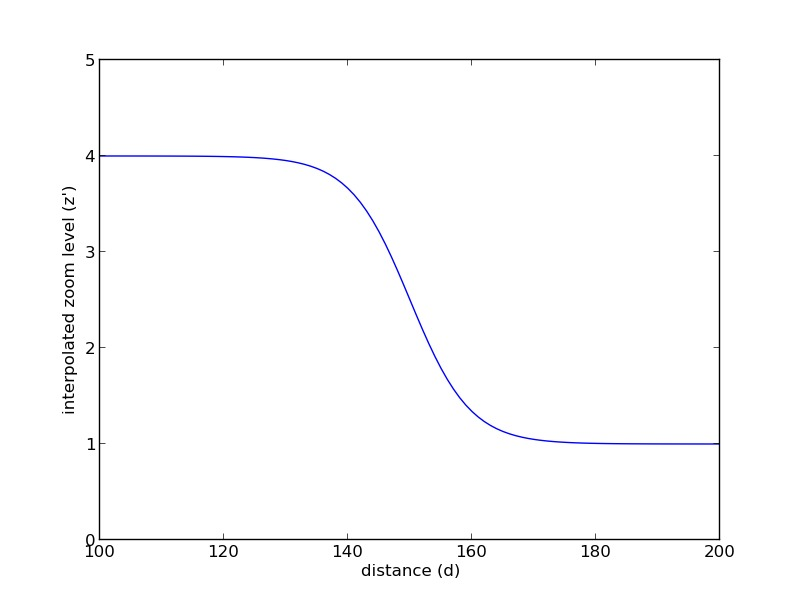
\includegraphics[width=0.8\linewidth]{img/logistic_graph.jpg}
    \caption[Logistic Graph]{Example graph of a logistic function with $\emph{$r_0$} = 100$, $\emph{$r_1$} = 200$, and $\emph{z} = 4$.}
    \label{fig:logistic_graph}
\end{figure}

The combined piecewise function for the distance function is shown below (Equation~\ref{eq:piecewise}).

\begin{equation}
    \label{eq:piecewise}
    f(d) = \left\{
        \begin{array}{lcr}
            d \times \frac{1}{z} & : & 0 < d < r_0 \\
            d \times \left( 1 + \epsilon + \frac{(z - 1 + 2\epsilon)}{1 + ae^{b(d-r_0)}}\right) & : & r_0 < d < r_1\\
            d & : & r_1 < d 
        \end{array}
    \right.
\end{equation}

A graph of the distances for the texture magnification functions is shown below in 
Figure~\ref{fig:texture_mag_graph} comparing the original distance and the computed distance.

\begin{figure}[htp] \centering
    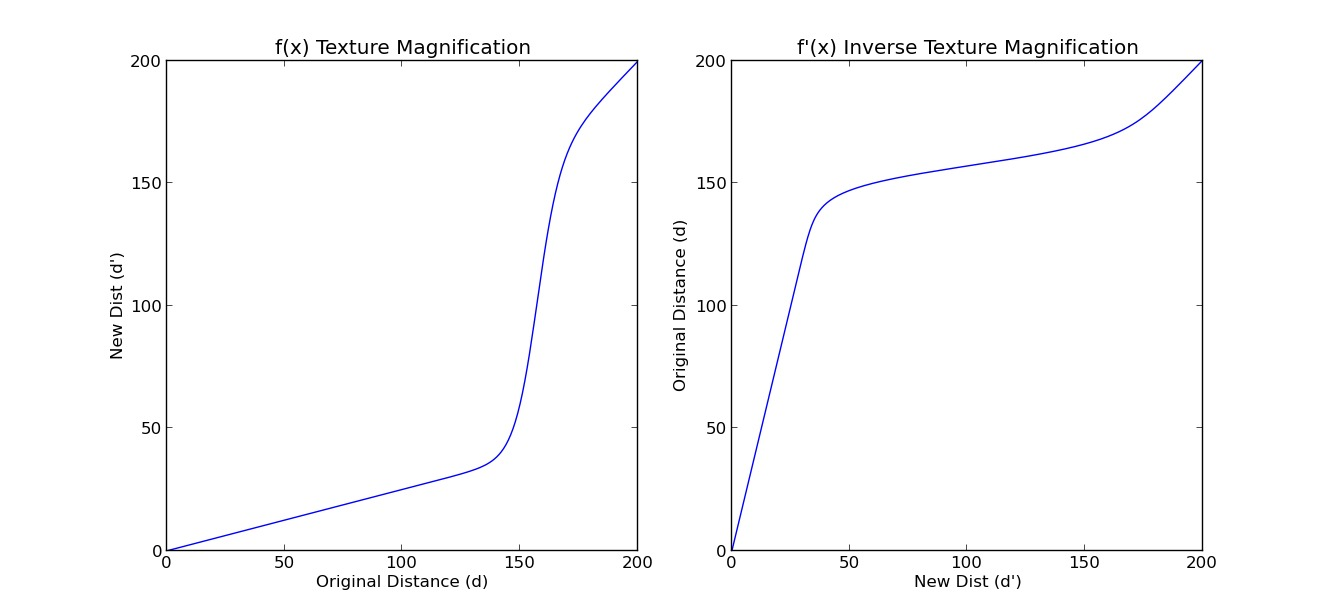
\includegraphics[width=0.8\linewidth]{img/full_graph.jpg}
    \caption[Distance Function]{Graph of the piecewise function, the x axis represents the original distance from 
    the mouse cursor and the y axis represents the new computed distance from the mouse cursor. The right image 
    is the graph of the inverse of the piecewise function. This figure shows that both functions have the same 
    domain and range.}
    \label{fig:texture_mag_graph}
\end{figure}

\section{Graph Magnification}
\label{section:graph_magnification}
To move the graph network correctly, we must use functions that are related to the texture magnification 
functions above. To perform magnification on a texture, we decrease the distance between the original UV coordinate and the focal point. If we decrease the distance between a cursor and a graph element, we cause the data to become clustered around the cursor instead of moving further away from the cursor.

Both functions map to the same domain and range. For any input between 0 and the outer radius, $r_1$, the output 
of the distance function should also be between 0 and $r_1$. The function for moving the graph network is also 
piecewise, much like the texture magnification functions.

If we examine the linear magnification function and its inverse for texture magnification, we can deduce that the correct way magnify the graph network is the 
inverse of the texture magnification function. The inverse of the linear magnification transformation (seen in 
Equation~\ref{eq:linear_magnification}) is trivial to compute, and is shown below in 
Equation~\ref{eq:inverse_linear_magnification}. The original function transforms values in the range of 0 to 
$r_0$ to 0 to $\frac{r_0}{z}$, so the inverse equation only accepts inputs in the range 0 to $\frac{r_0}{z}$.

\begin{equation}
    \label{eq:inverse_linear_magnification}
    g(d) = d \times {z}
\end{equation}

While the linear equation is trivial to invert, the logarithmic function is impractical to do analytically. The 
simplified version of the non-linear texture magnification is shown in Equation~\ref{eq:simple_log}. Solving this 
problem requires using Lambert W functions \cite{Corless1996}. Solving this equation was outside of the scope of the thesis, so we avoid solving this problem analytically by solving Equation~\ref{eq:modified_logistic} and storing the values in an 
array. Retrieving the values from the array uses a binary search to find the solution. For our purposes, we stored every value in the range from $r_0$ to $r_1$ with an interval of $0.1$. This interval was discovered by viewing the derivative of the texture magnification function.

\begin{equation}
    \label{eq:simple_log}
    f(d) = de^{d}
\end{equation}

The full piecewise function for graph magnification is seen below, $BinarySearch(z,d)$ corresponds to the index in the table given by performing a binary search of the table with a zoom level, \emph{z}, for a particular distance, \emph{d}. Because we only store values from $r_0$ to $r_1$, we add $r_0$ to this value to get the answer for the inverse of the non-linear function.

\begin{equation}
    \label{eq:inv_piecewise}
    g(d) = \left\{
        \begin{array}{lcr}
            d \times z & : & 0 < d < \frac{r_0}{z} \\
            BinarySearch(z,d) + r_0 & : & \frac{r_0}{z} < d < r_1\\
            d & : & r_1 < d 
        \end{array}
    \right.
\end{equation}


\section{Multi-cursor Magnification}
\label{section:multi_cursor}

The techniques described in the previous sections (Section~\ref{section:texture_magnification} and~\ref{section:graph_magnification}) are all applicable for
situations where only a single mouse cursor is applied within $r_1$ pixels of the cursor. The formulas 
described above are extensible and only need to be modified slightly for usage when multiple cursors affect
a fragment or graph element.

Intuitively, we would expect that cursors closer to a point should have more of an effect on the final
position of a fragment or graph element than cursors that are further away. This intuition leads to one possible
solution of performing a weighted average to get a final position.

Instead of simply returning a new distance from the texture and graph magnification functions 
(Equations~\ref{eq:piecewise} and~\ref{eq:inv_piecewise}), we have each function return two values, 
the original distance and the vector corresponding to the direction it would have been moved in. 

Because we want cursors that are closer to the element being affected to have a stronger influence, we
assign a higher weight to cursors that are closer, a full equation is seen below 
(Equation~\ref{eq:weighted_cursors}). It is important to note that the weights add up to 1.0, as we should not
move a point more than it can be transformed by the single application of the magnification equations.

\begin{figure}[htp] \centering
    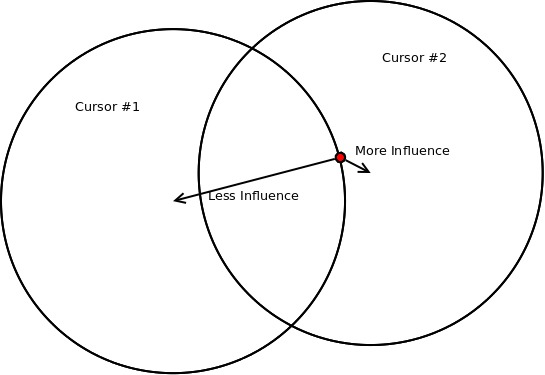
\includegraphics[width=0.6\linewidth]{img/multi_cursor.jpg}
    \caption[Multiple Cursor Magnification]{The two regions of magnification are seen overlapping a particular red point. Cursor 2 should have a higher weight when determining the final position, as it is closer to the original position of the point.}
    \label{fig:multi_cursor}
\end{figure}

\begin{equation}
    \label{eq:weighted_cursors}
    w_i = \frac{r_1 - d_i}{\sum\limits_{i=1}^n (r_1 - d_i)}
\end{equation}

\begin{equation}
    \label{eq:weighted_sum}
    \vec{v'} = \sum\limits_{i=1}^n w_i \vec{v_i}
\end{equation}

The vectors are multiplied by the corresponding weight, and the resulting vector is added to the original point
to get the new position of the element (Equation~\ref{eq:weighted_sum}). $\vec{v_i}$ the result of multiplying
the result of the piecewise function (Equation~\ref{eq:piecewise}) for texture magnification or graph manipulation
(Equation~\ref{eq:inv_piecewise}) by the normalized direction to the cursor $\vec{c_i}$.

\begin{figure}[htp] \centering
    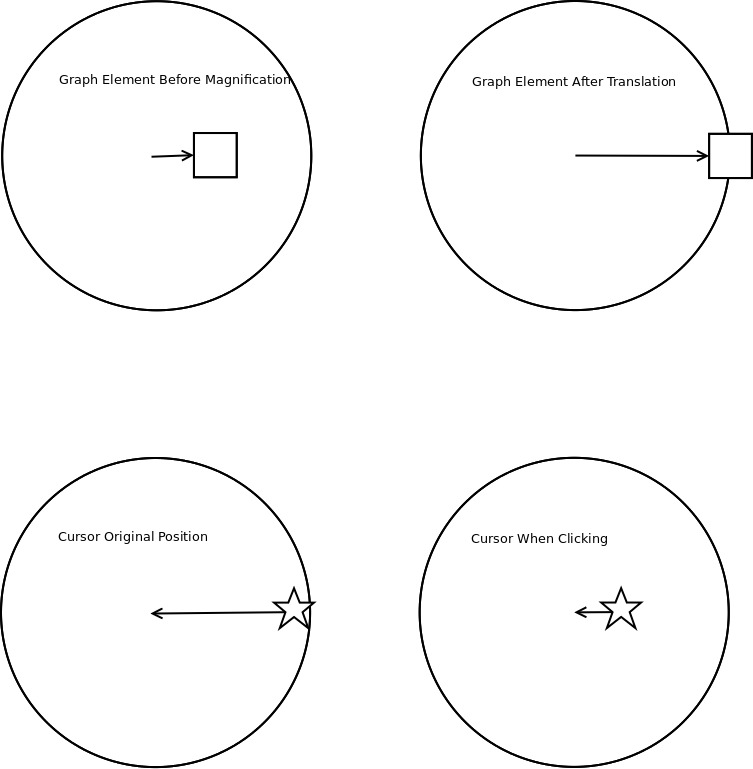
\includegraphics[width=0.6\linewidth]{img/clicking.jpg}
    \caption[Interacting with Magnified Elements]{The circular region represents the area magnified by a cursor at its center. The magnification that moves the graph element must be inverted to allow users to click on the actual position of the graph element, as seen in the bottom half of the image.}
    \label{fig:clicking}
\end{figure}

When interacting with the visualization application without magnification, every cursor is assumed to be directly over a point in screen space. However, when graph elements are moved due to being magnified by a cursor, we must compensate for the magnified position to interact with the node accordingly. Seen in Figure~\ref{fig:clicking}, we perform the texture magnification equations on a cursor to find the original position of a graph element. This occurs only when clicking on a graph
element, the cursor does not actually change its position on the screen.

\section{Summary}
\label{subsection:magnification_summary}

This chapter detailed the main magnification function used for our application for both satellite images and the graph network. A method for applying this function when multiple points of focus are included is also described. The following chapter discusses the application's overall performance and a short survey of responses to the new system.


%%%%%%%%%%%%%%%%%%%%%%%%%%%%%%%%%%%%%%%%%%%%%%%%%%%%%%%%%%%%%%%%%%% 
%                                                                 %
%                           RESULTS                               %
%                                                                 %
%%%%%%%%%%%%%%%%%%%%%%%%%%%%%%%%%%%%%%%%%%%%%%%%%%%%%%%%%%%%%%%%%%% 
 
% \specialhead{INTRODUCTION}
\chapter{RESULTS}
\label{chapter:results}

In the previous two chapters, we discussed the changes to the overall visualization systems as well as the methods to perform non-linear magnification on our dataset. This chapter presents the resulting visualization of the entire application, various performance statistics, and a brief survey of opinions regarding the magnification effect.

\section{Images}
\label{section:image_results}

Figure~\ref{fig:s_r_no_zoom} displays the visualization of an area of just the road network and satellite images. This image is what is stored in the FBO while this region is being viewed. Figure~\ref{fig:s_r_mag} shows successively higher levels of magnification around a single cursor. The red and blue visualization is a debugging tool to indicate which areas are under linear magnification (red) and which are under non-linear magnification (blue). The outer radius is set to 400 pixels and the inner is set at 200 pixels for these images. As the magnification increases, the area being magnified becomes more pixelated. This is due to the limited resolution of the original texture stored in the FBO\@. As we perform magnification, fewer individual pixels of the source texture are being used for the same region. 

To provide a high resolution image at these high levels of magnification, we can render the scene multiple times based on the different magnification levels utilized by the users. If we attempt to store the same geographic layer at $n$ times the current level of detail, we produce an image that is $n^2$ as big as the current texture. We are using RGB values for the texture, which results in $3 * width * height$ bytes for each original texture with a viewport of $width$ by $height$ pixels. We currently run the application at a 1600 x 1000 resolution, which requires 4.5 MB of data on the GPU\@. Most modern GPUs allow for between 2 GB to 4 GB
of data on the GPU at any time; this means that we cannot simply render all the data to the GPU for a given geographic region, as we currently allow for a 72x linear magnification. This magnification would require 22 GB of storage on the GPU.

We can begin to avoid this memory issue by only storing the higher resolution images in regions that are near cursors. However, there still may be problems with performing this rendering multiple times for each cursor, for each frame. Currently, we allow for 45 discrete levels of linear magnification, so we should only calculate these high resolution region for the current level of linear magnification of the cursor  as well as its neighboring values. 

\begin{figure}[htp] \centering
    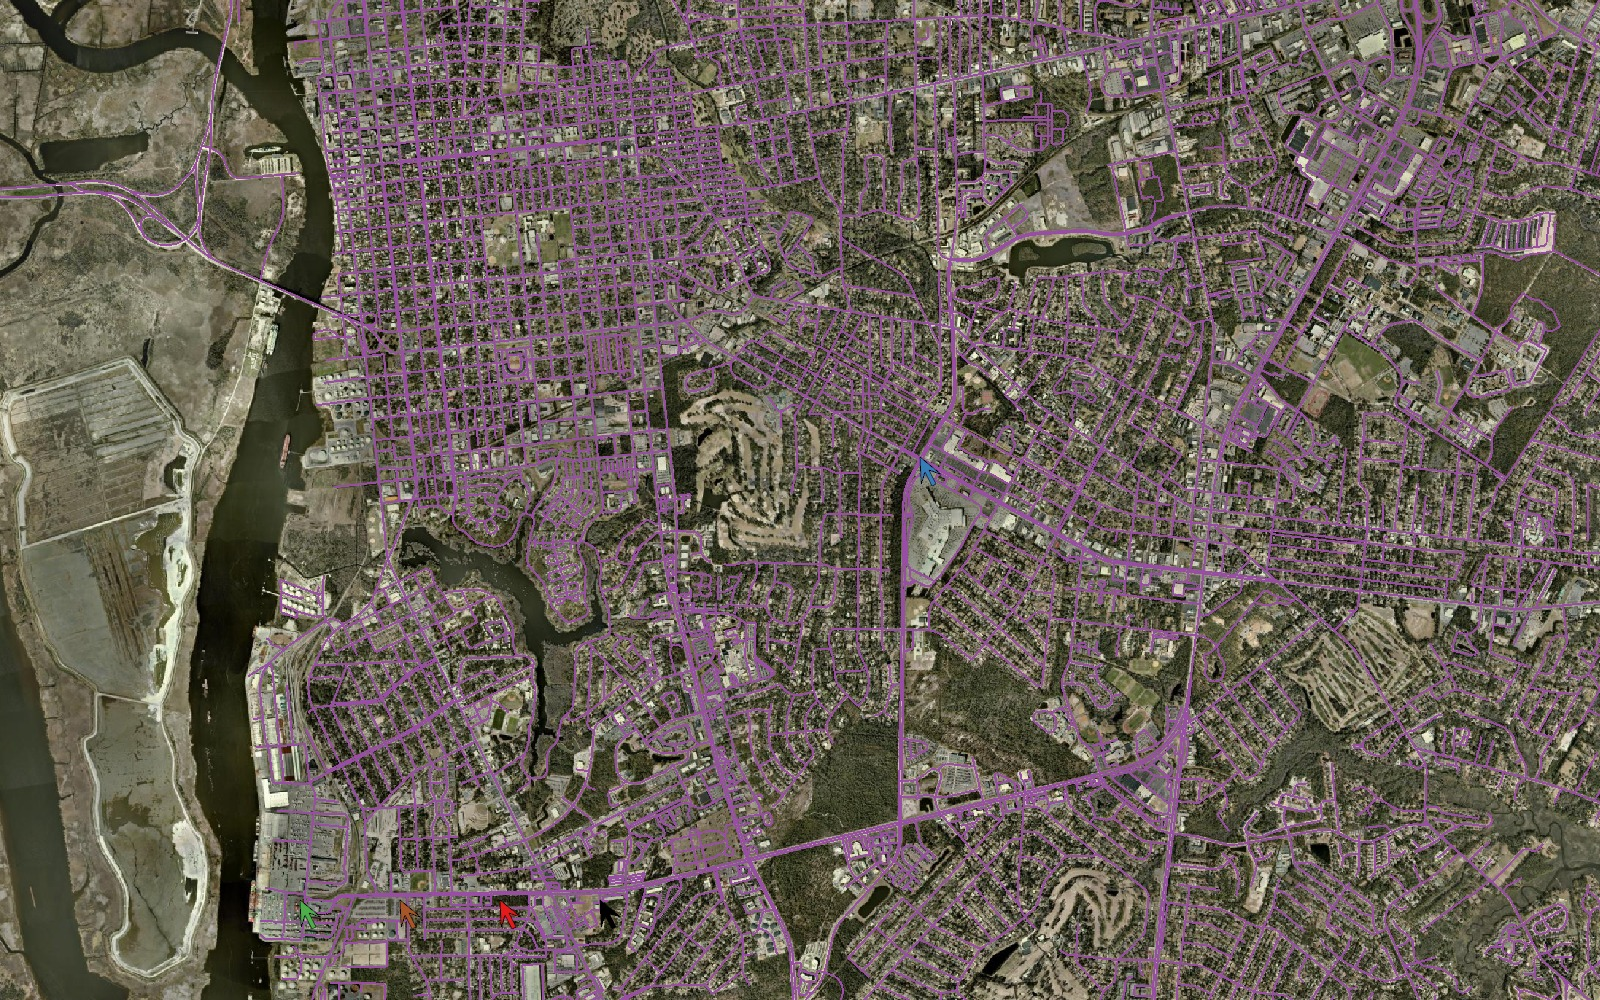
\includegraphics[width=1.0\linewidth]{img/s_r_no_zoom.jpg}
    \caption[Satellite Images and Road Network without Magnification]{A single image showing a section of the application with just the road network and satellite images. This is the current contents of the FBO, and is transformed by the magnification functions to produce the images in Figure~\ref{fig:s_r_mag}.}
    \label{fig:s_r_no_zoom}
\end{figure}

\begin{figure}[htp] \centering
    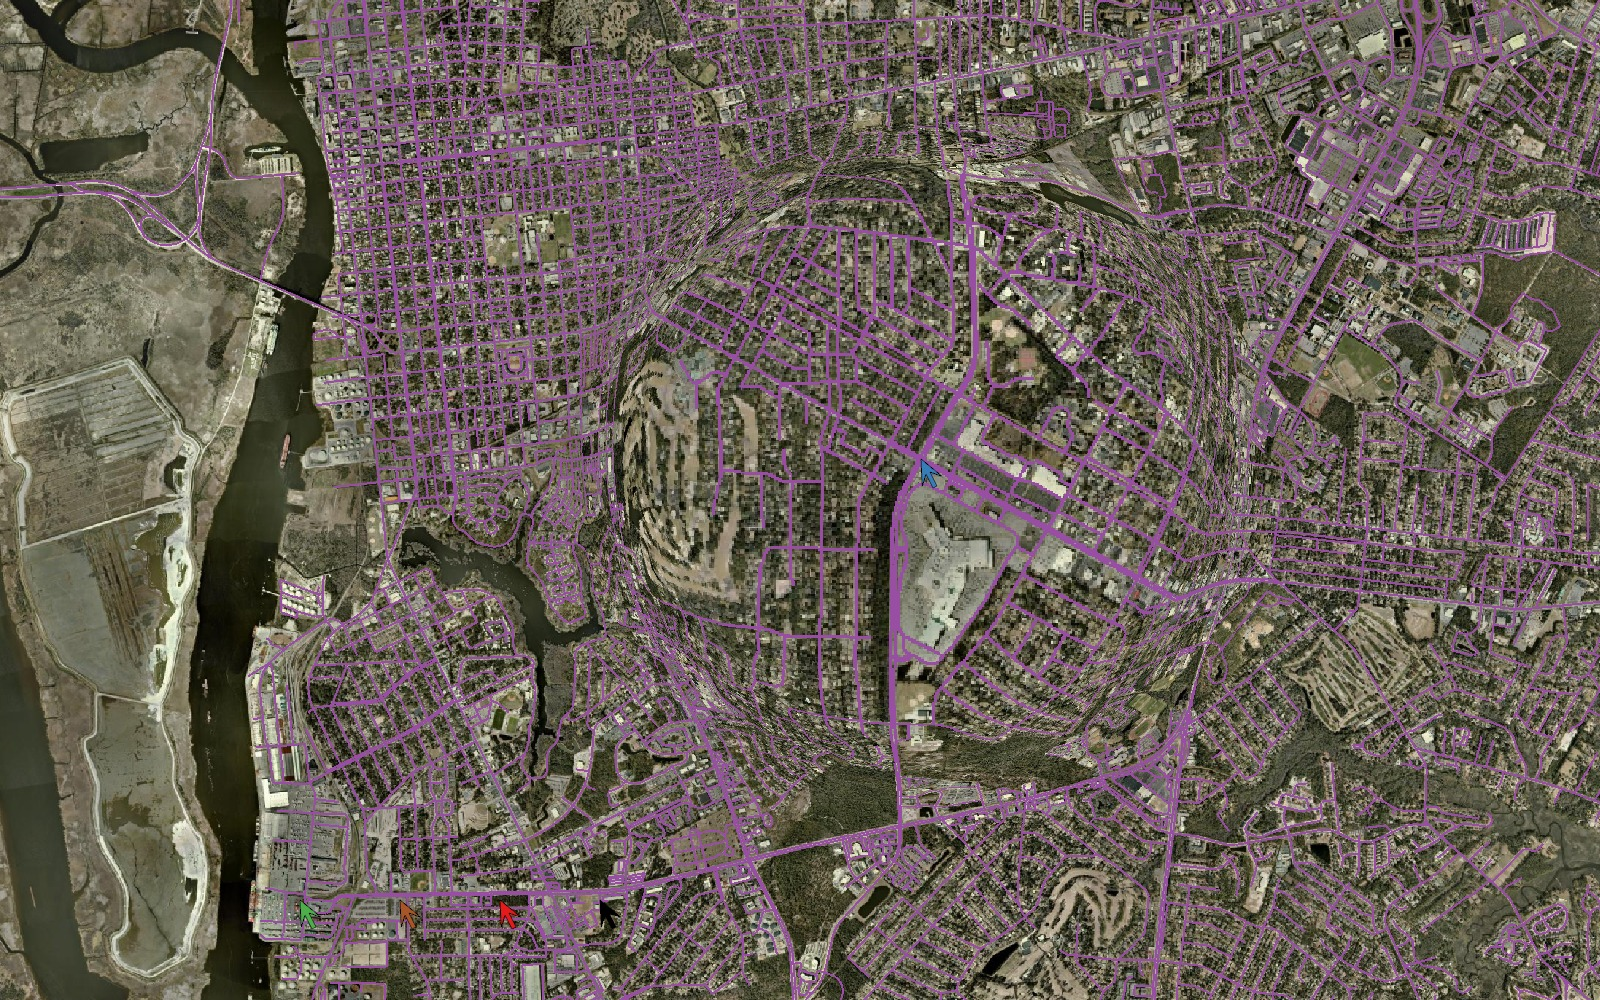
\includegraphics[width=0.49\linewidth]{img/s_r_5_zoom.jpg}
    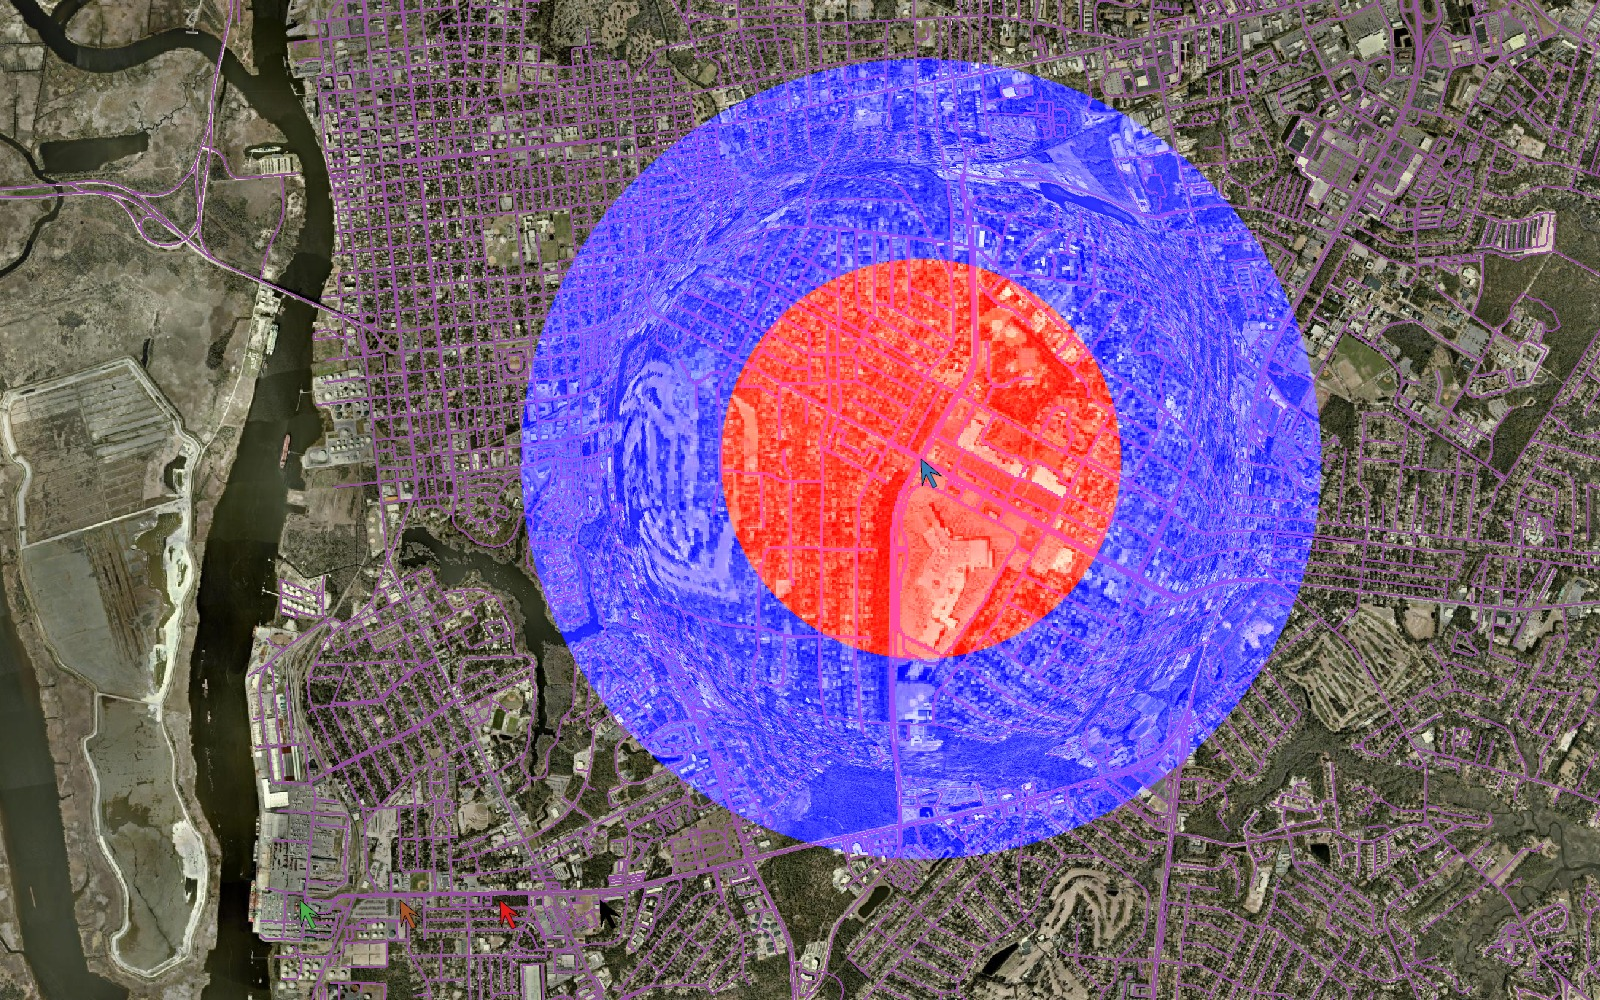
\includegraphics[width=0.49\linewidth]{img/s_r_5_zoom_color.jpg}
    \vspace{3 mm}

    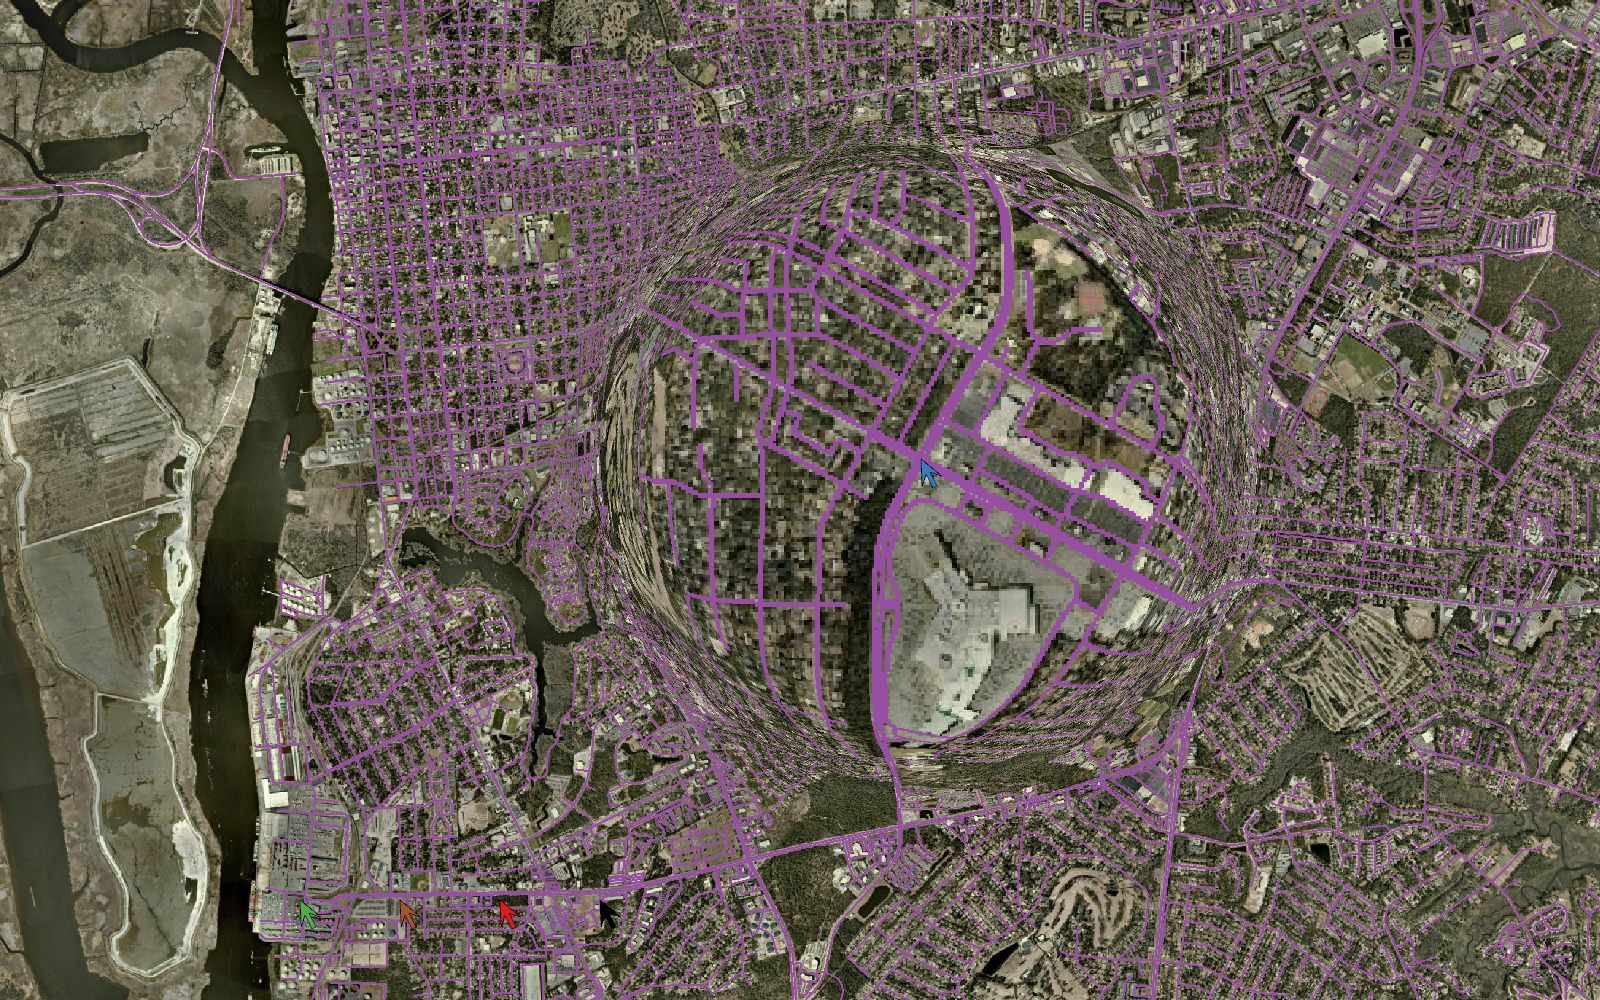
\includegraphics[width=0.49\linewidth]{img/s_r_10_zoom.jpg}
    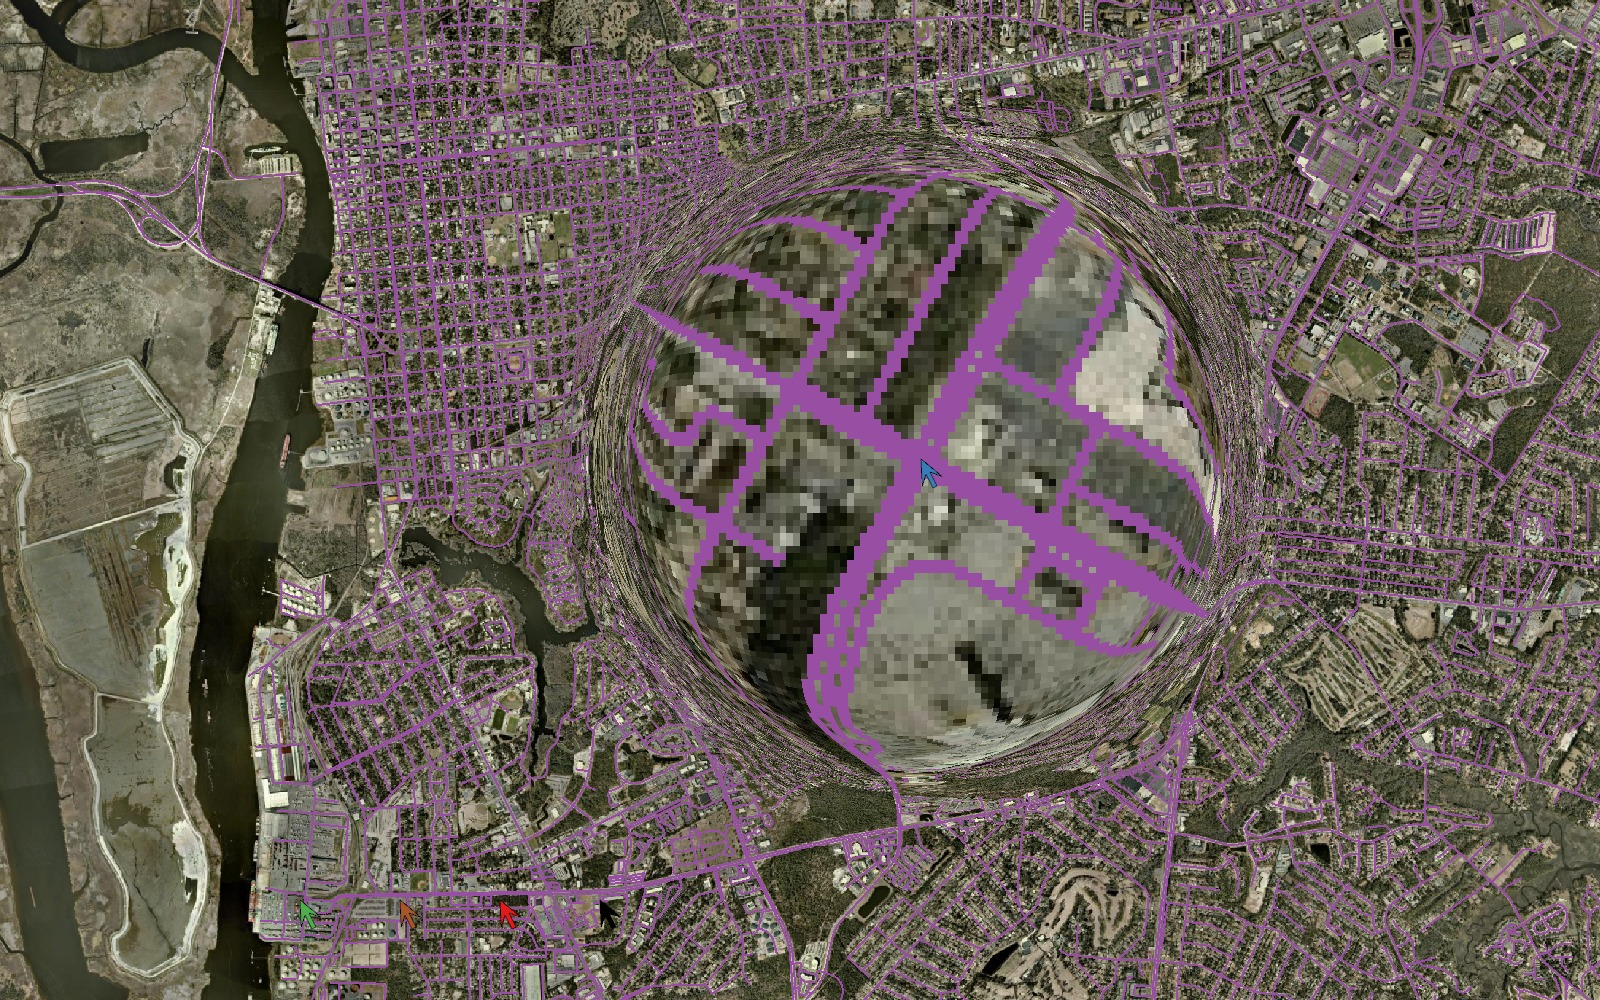
\includegraphics[width=0.49\linewidth]{img/s_r_20_zoom.jpg}
    \vspace{3 mm}

    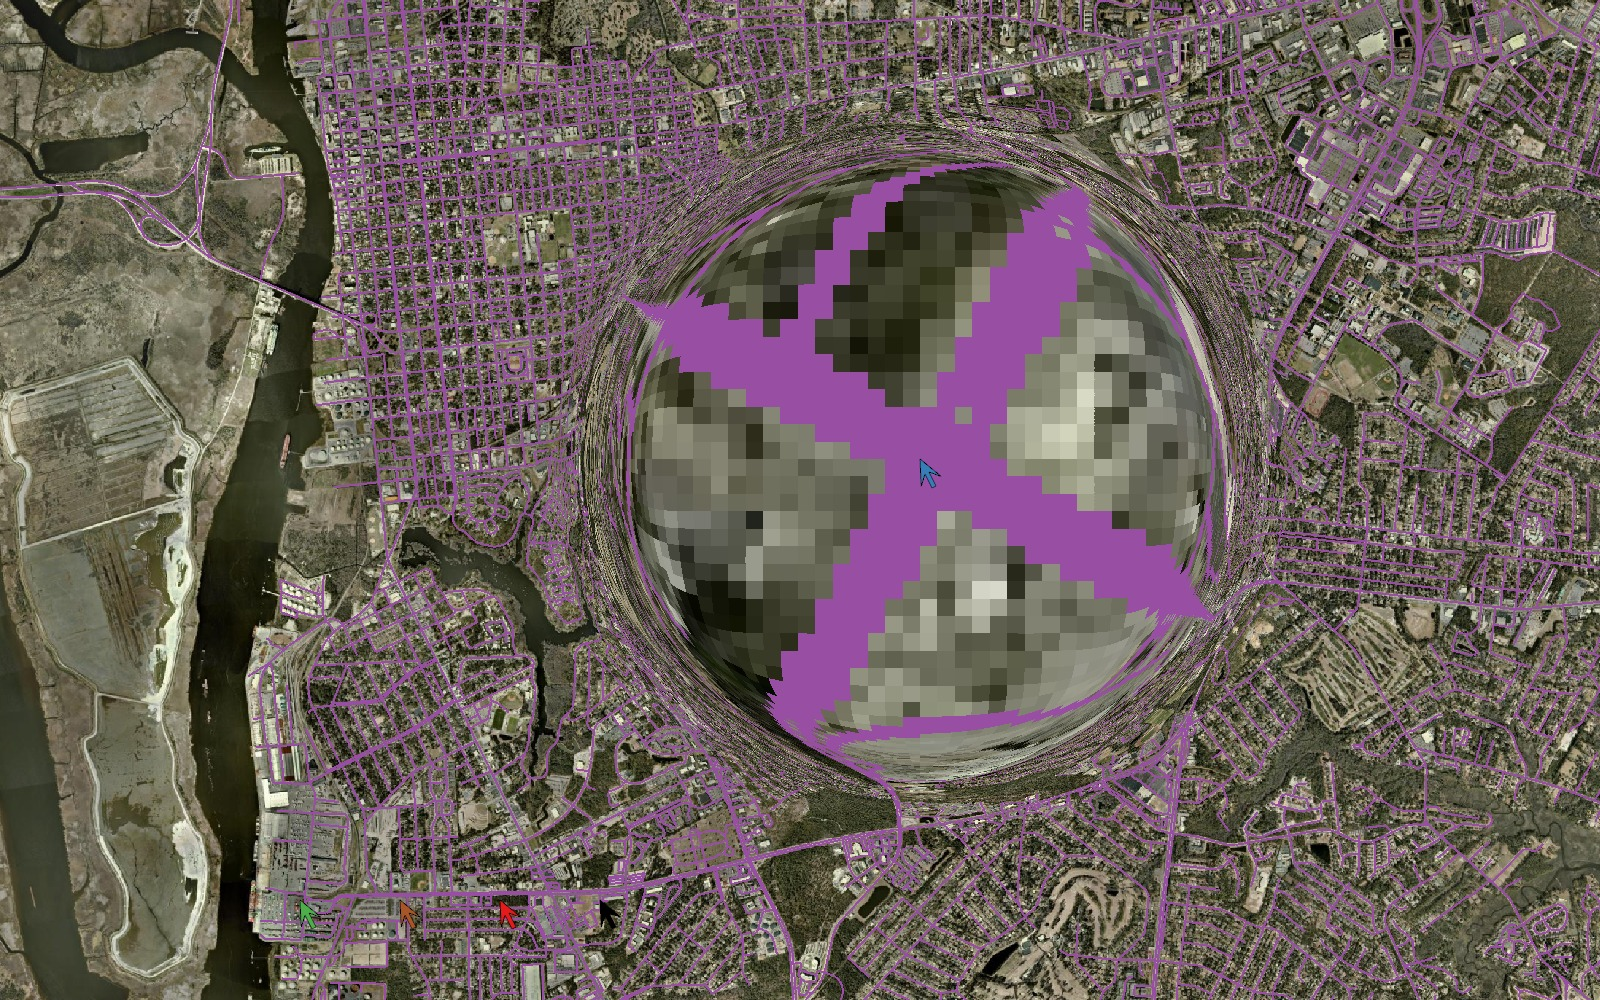
\includegraphics[width=0.49\linewidth]{img/s_r_30_zoom.jpg}
    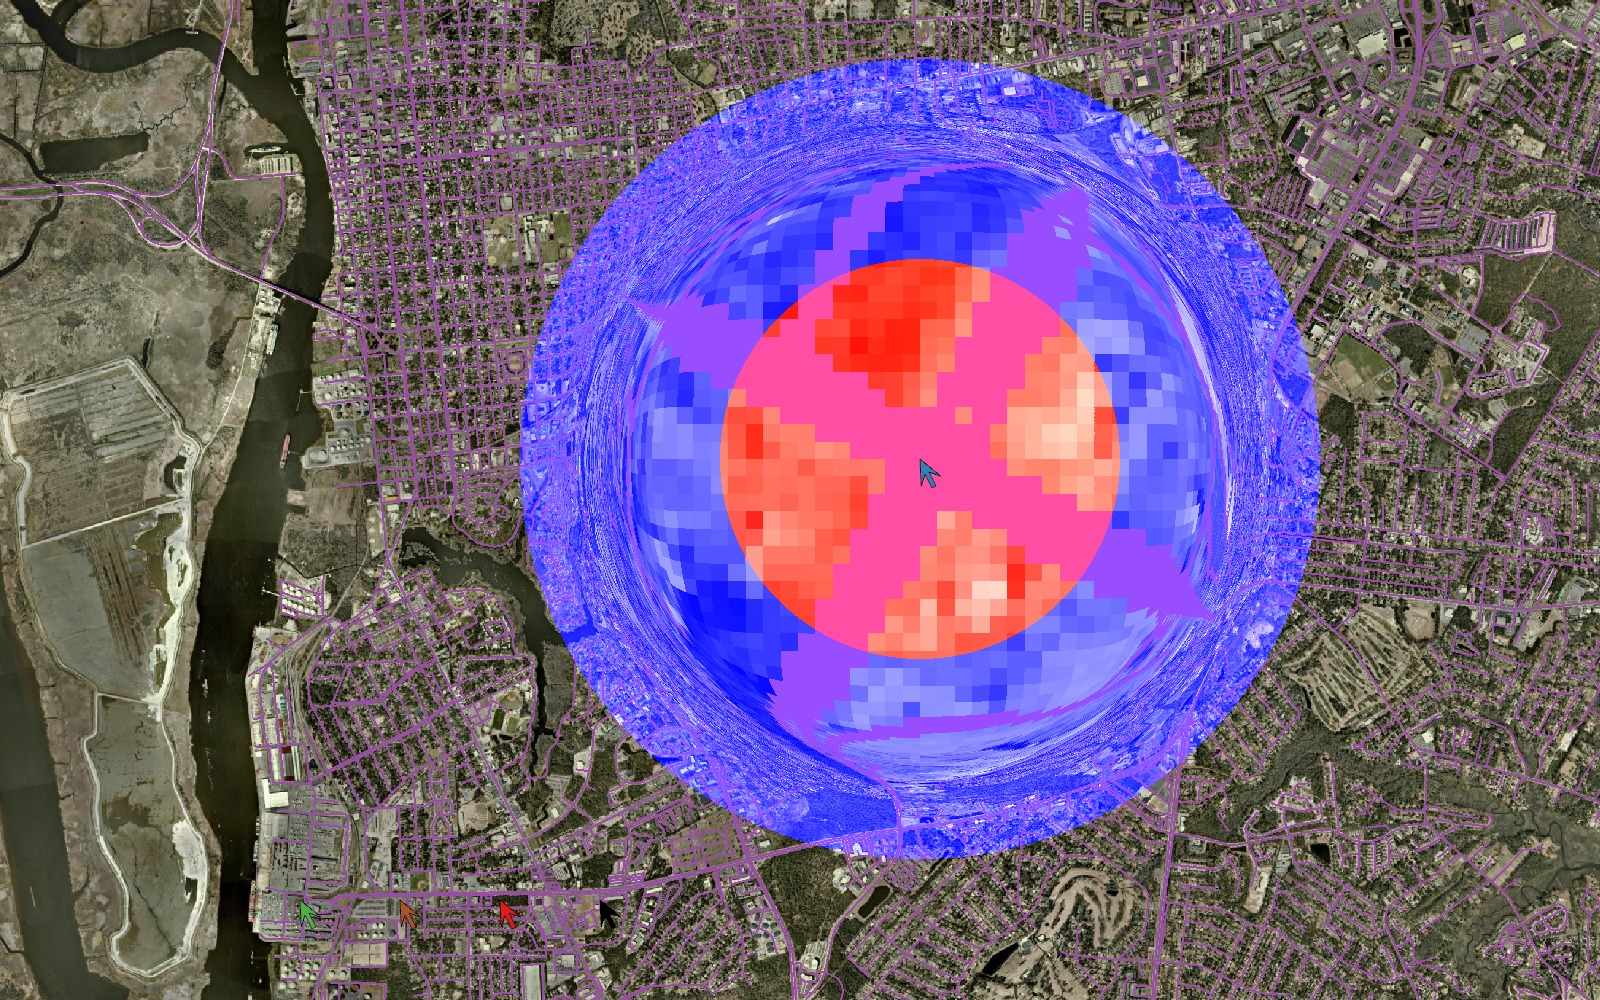
\includegraphics[width=0.49\linewidth]{img/s_r_30_zoom_color.jpg}
    \caption[Satellite Images and Road Network with 1.6x to 17.4x Linear Magnification]{This series of images 
    shows the road network and satellite images rendered at increasing levels of linear magnification, ranging 
    from 1.6x to 17.4x. Notice that the individual pixels become more noticeable as we increase the zoom. The 
    blue region represents the area of non-linear magnification, while the red region represents the area of 
    linear magnification. This is a debugging visualization for viewing the different regions of magnification.}
    \label{fig:s_r_mag}
\end{figure}

Figure~\ref{fig:s_r_g_no_zoom} shows the application without any magnification applied for a particularly dense area of graph elements. The user would like to see the individual elements separated and also see the underlying satellite imagery of the region. Figure~\ref{fig:s_r_g_mag} shows a series of images with an increasing level of linear zoom. By performing this magnification, the user is able to see the individual street and intersection information that was initially
obscured by the graph elements. As we increase the magnification of this region, the majority of the nodes become clustered in the non-linear region. Using a high magnification for these areas may end up being as detrimental as no magnification for multiple users, as the nodes are still indistinguishable from one another due to the demagnification of the blue region.

\begin{figure}[htp]\centering
    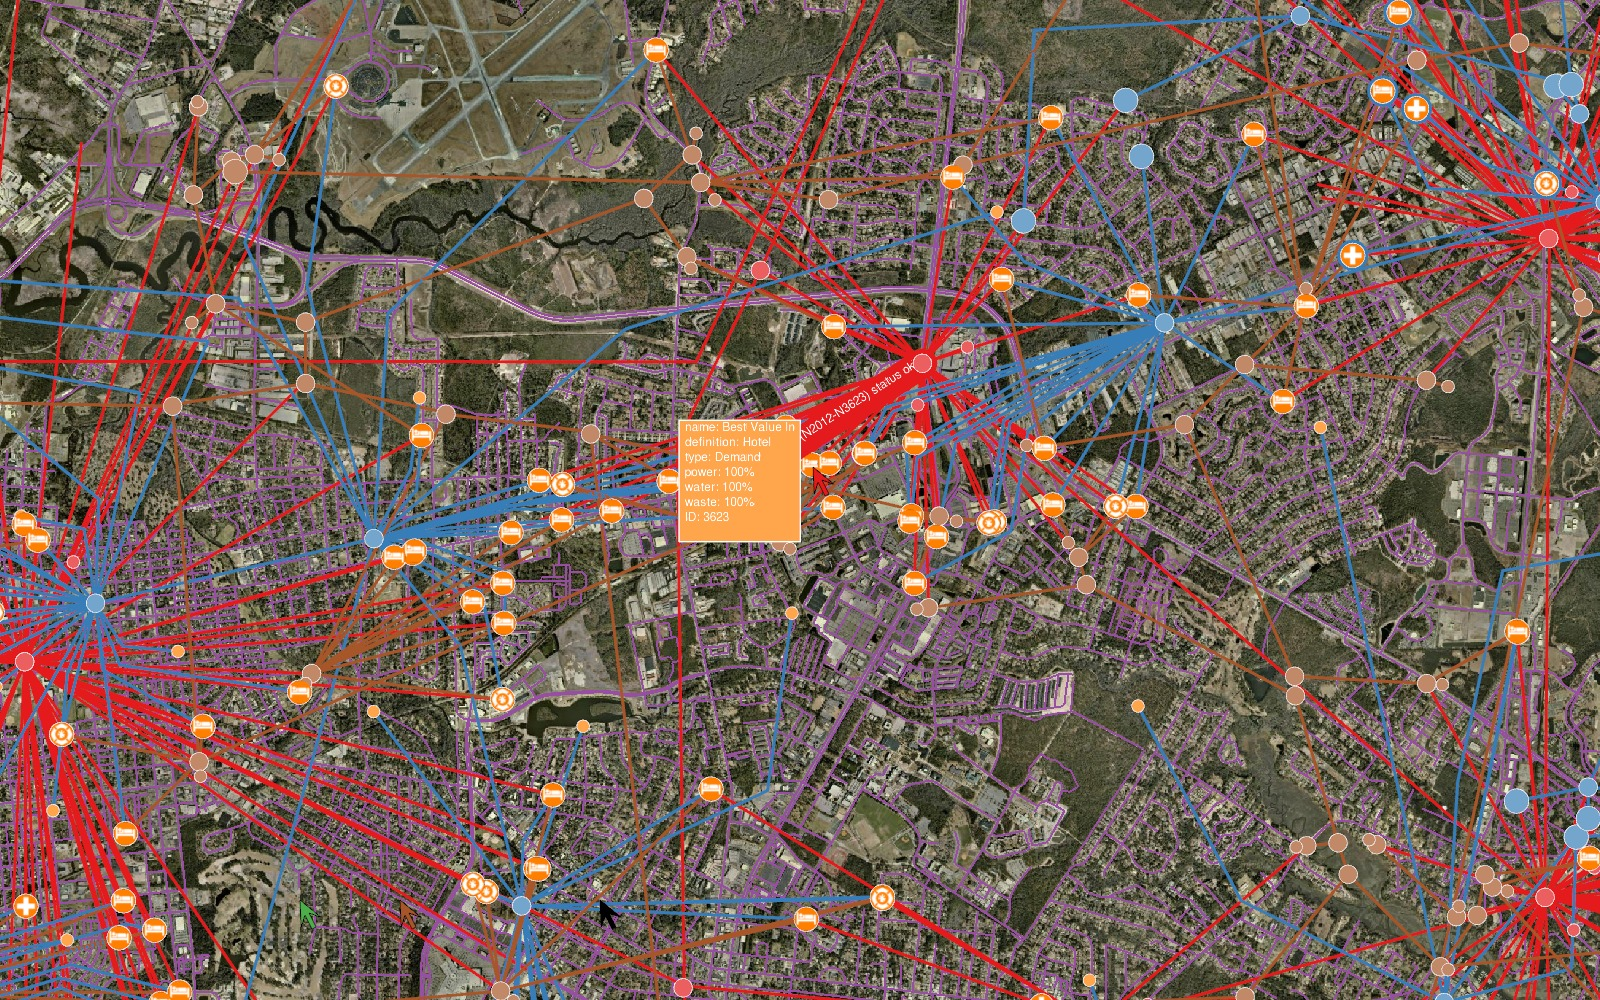
\includegraphics[width=1.0\linewidth]{img/s_r_g_no_zoom.jpg}
    \caption[Full Application without Linear Magnification]{A single image showing the application with the satellite images, graph network, and road network all displaying. This image is included as a base reference point for the images in Figure~\ref{fig:s_r_g_mag}.}
    \label{fig:s_r_g_no_zoom}
\end{figure}

\begin{figure}[htp]\centering
    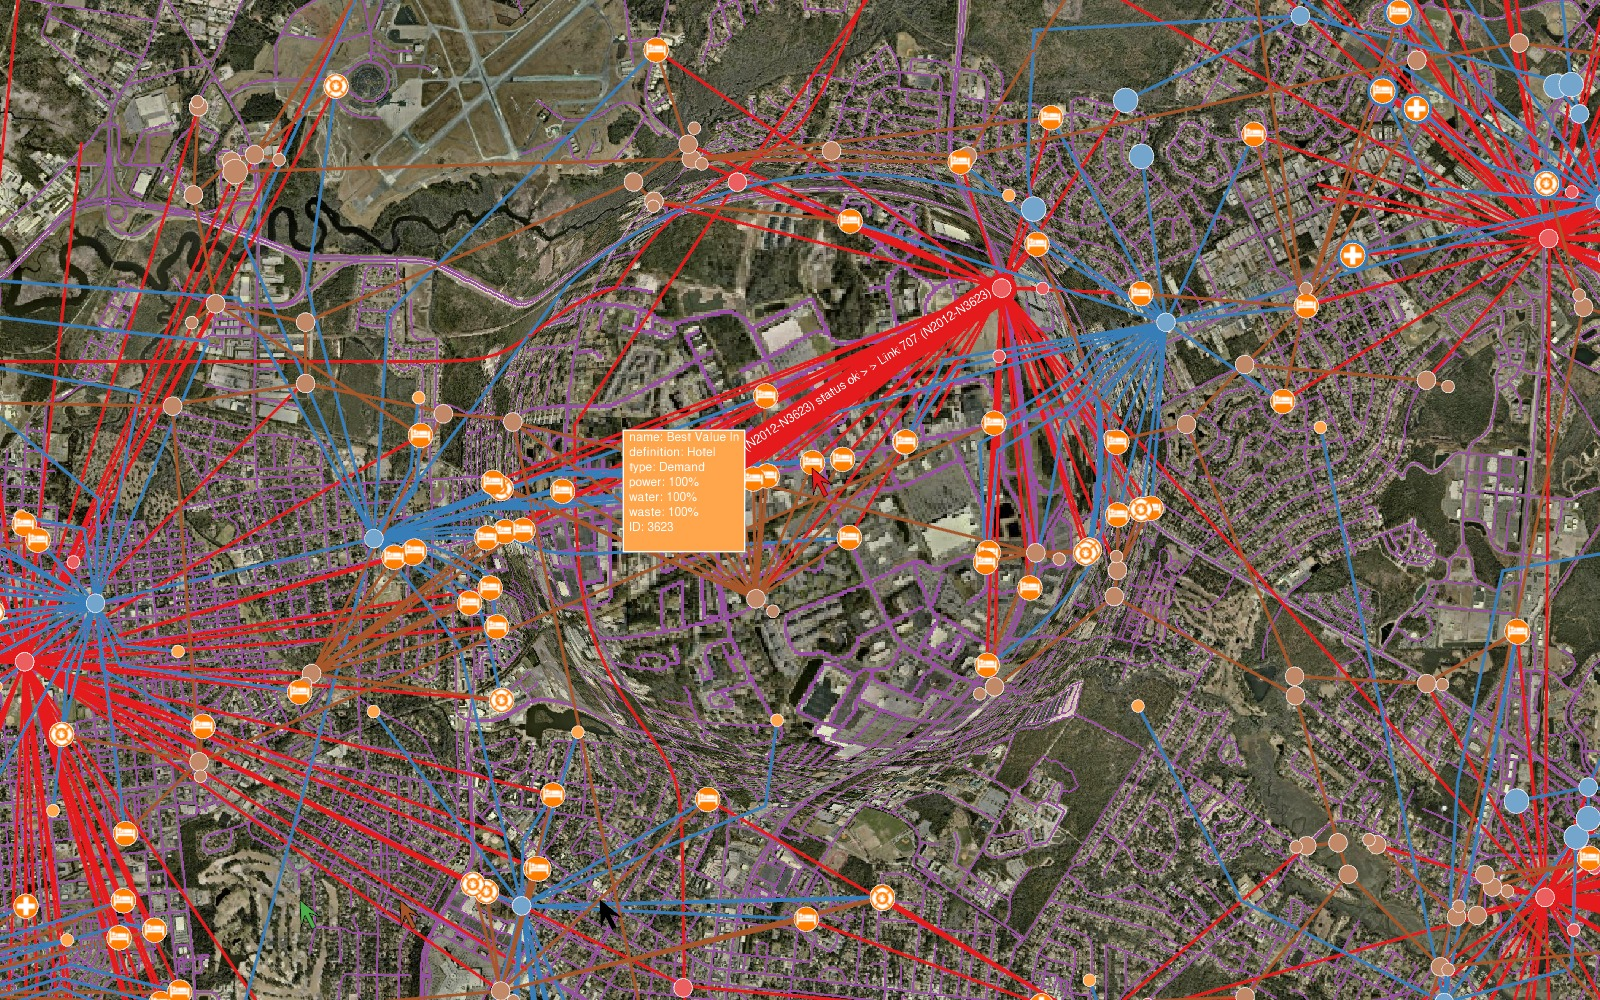
\includegraphics[width=0.49\linewidth]{img/s_r_g_5_zoom.jpg}
    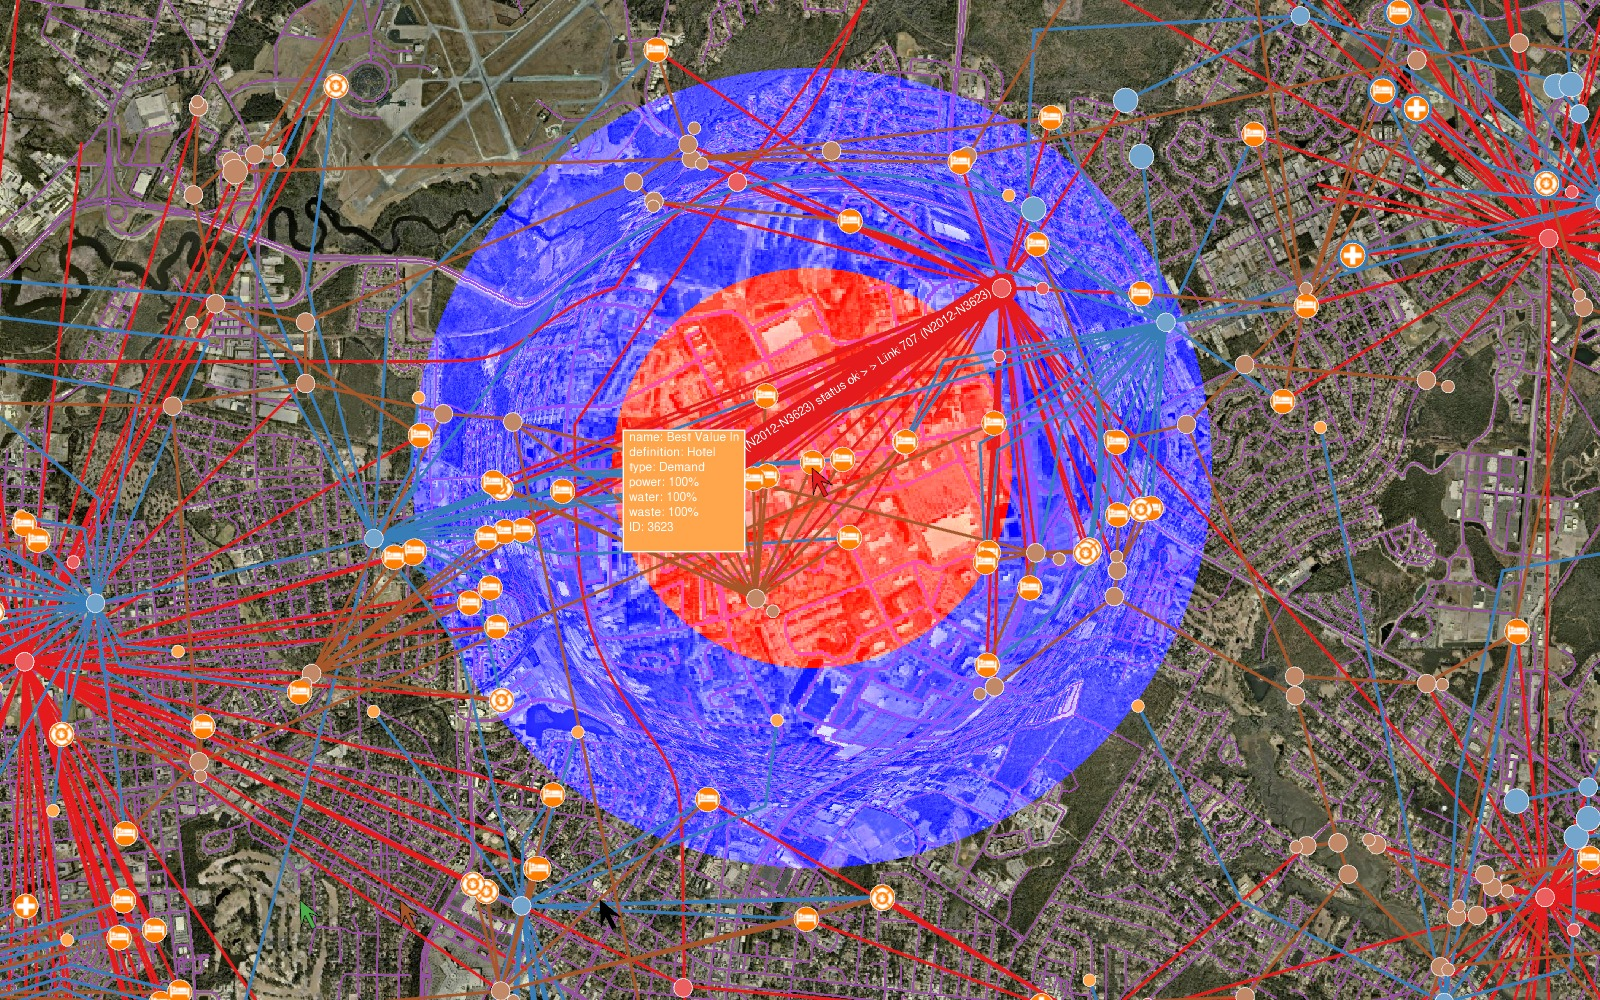
\includegraphics[width=0.49\linewidth]{img/s_r_g_5_zoom_color.jpg}
    \vspace{3 mm}

    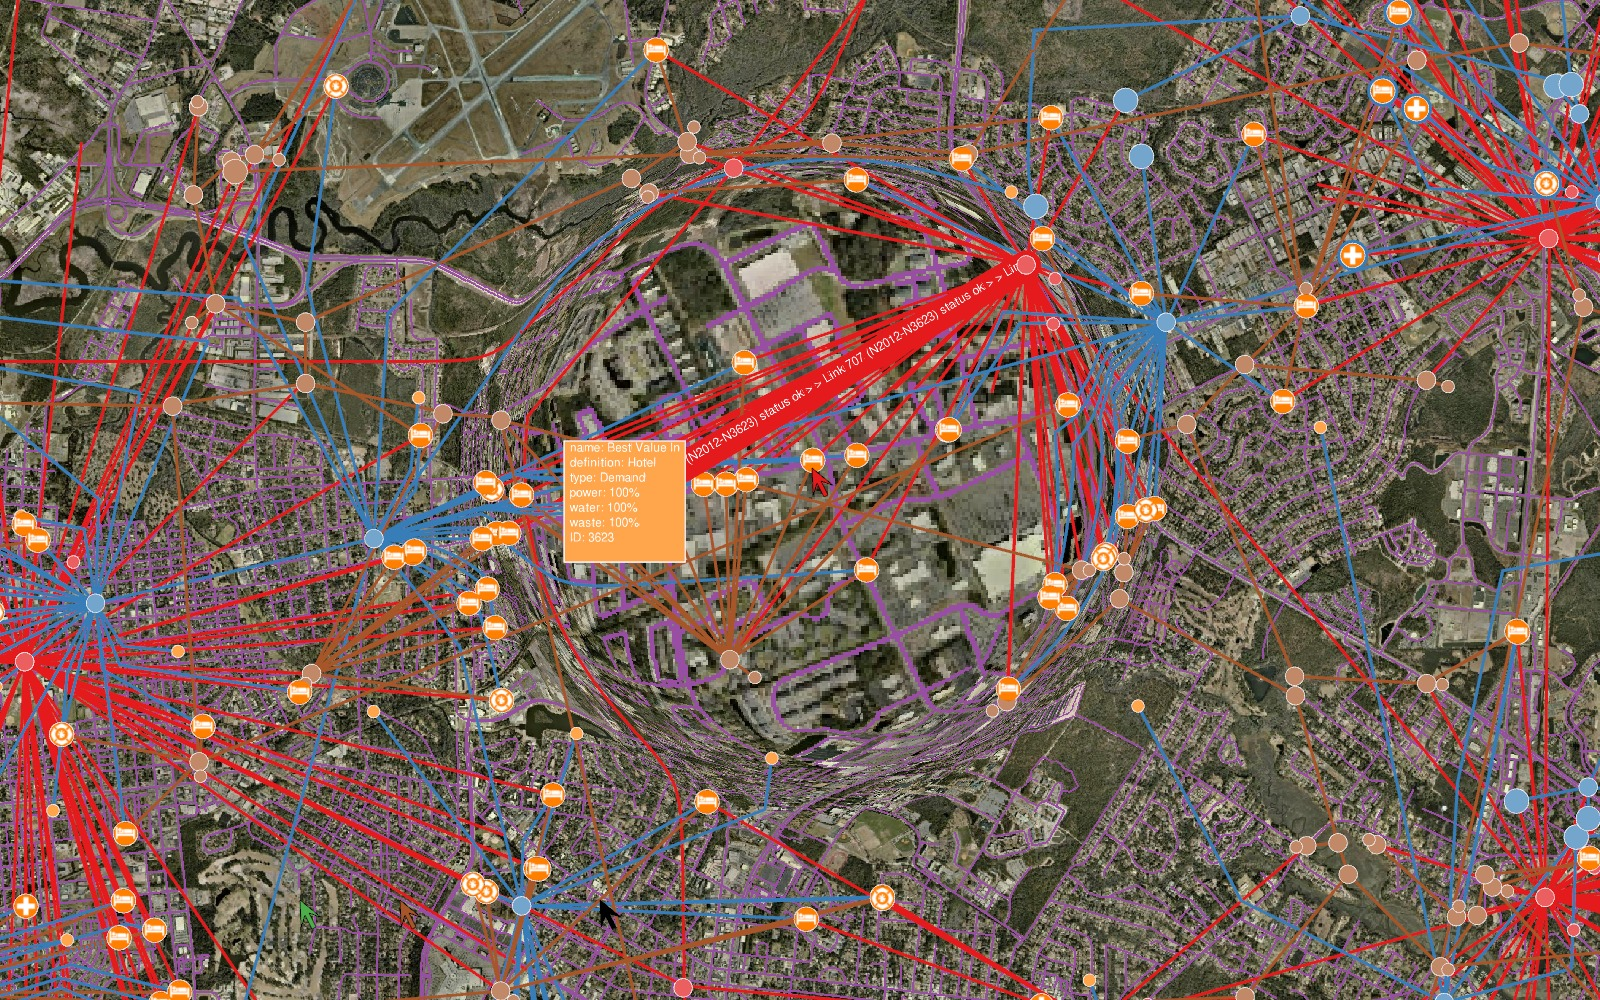
\includegraphics[width=0.49\linewidth]{img/s_r_g_10_zoom.jpg}
    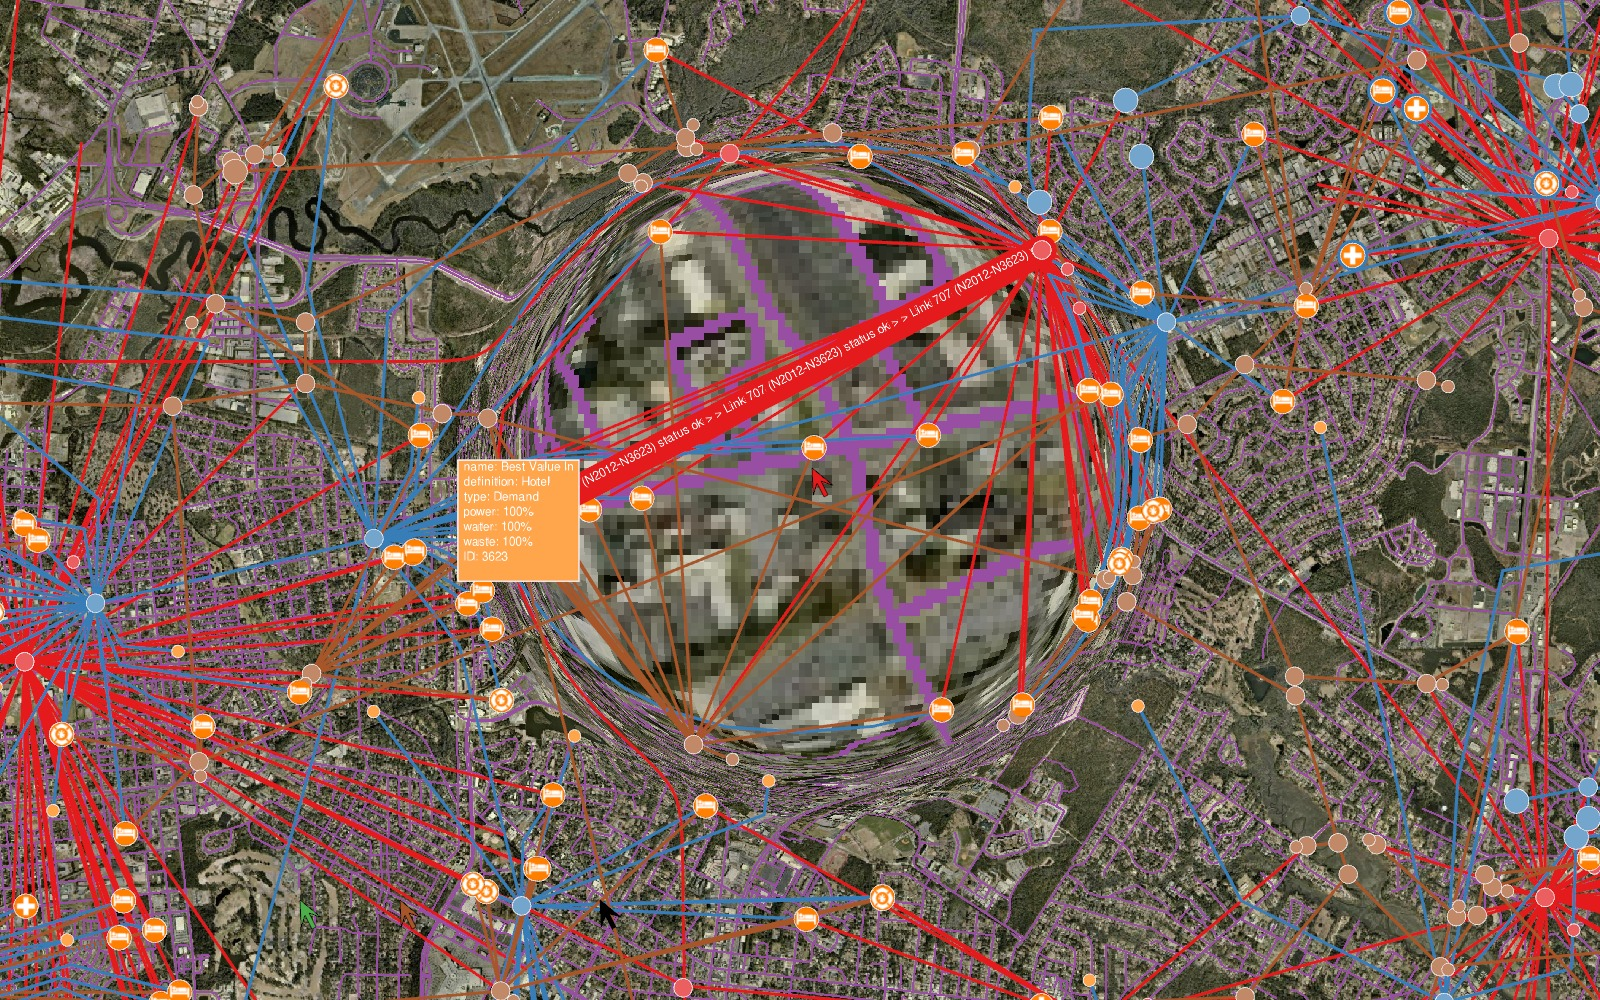
\includegraphics[width=0.49\linewidth]{img/s_r_g_20_zoom.jpg}
    \vspace{3 mm}

    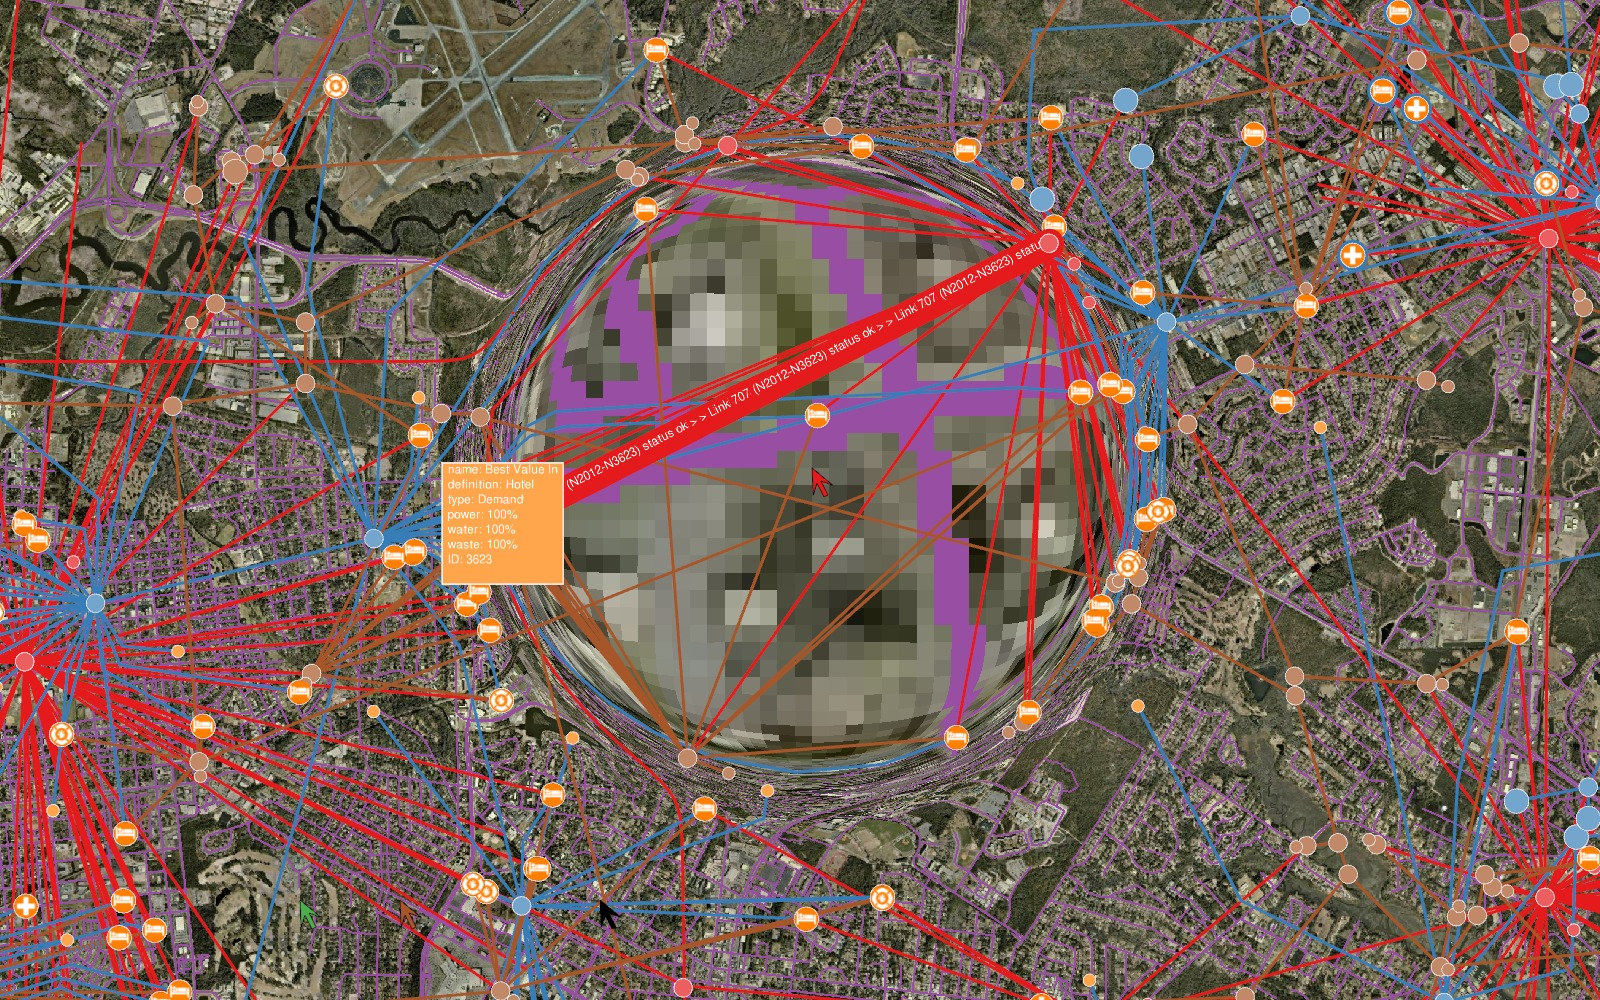
\includegraphics[width=0.49\linewidth]{img/s_r_g_30_zoom.jpg}
    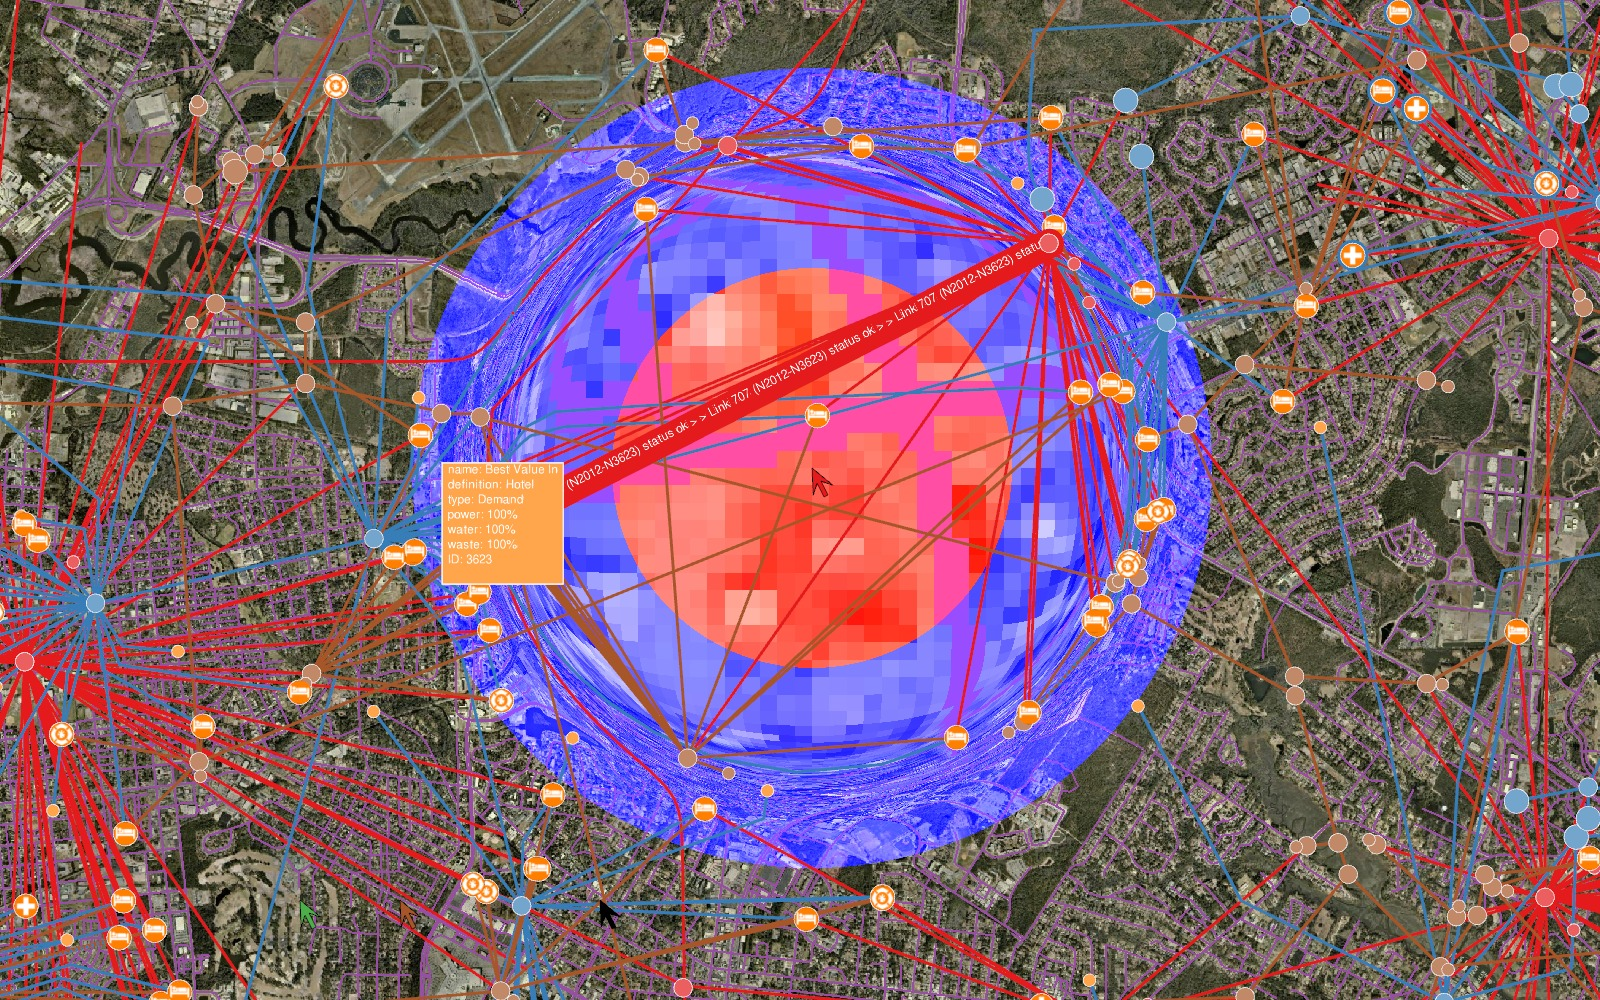
\includegraphics[width=0.49\linewidth]{img/s_r_g_30_zoom_color.jpg}
    \caption[Full Application with 1.6x to 17.4x Linear Magnification]{These images show the full application with an increasing level of linear magnification affecting both the graph data and the satellite images. The user is currently diagnosing a problem with the group of hotels in this region.}
    \label{fig:s_r_g_mag}
\end{figure}

The interaction between multiple magnification areas is seen in Figure~\ref{fig:problem_solving}. Both users are diagnosing a problem in the same area, and are able to see the region around their cursors in greater detail without affecting the other user. Note that the river between the two sites is still clearly visible, along with the edges between elements for both regions. This functionality allows the individual users to still see the relationship between their specific graph
elements to the overall system, further assisting in diagnosing the problems within the region.

\begin{figure}[htp]\centering
    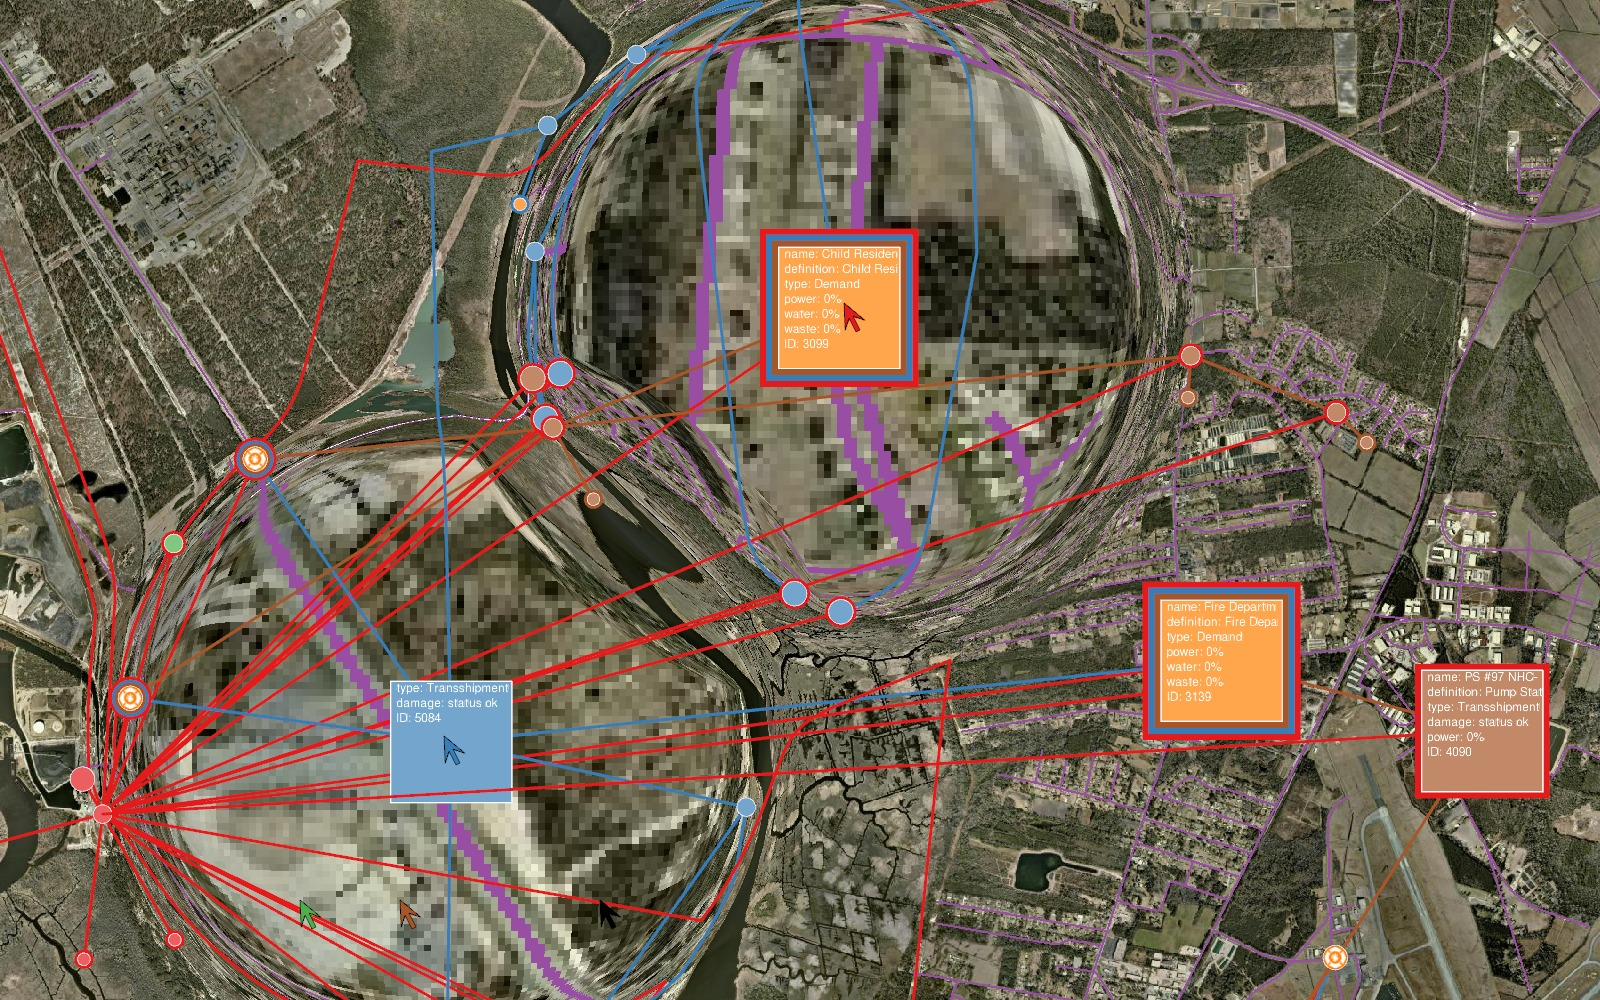
\includegraphics[width=0.49\linewidth]{img/problem_solving_20_20.jpg}
    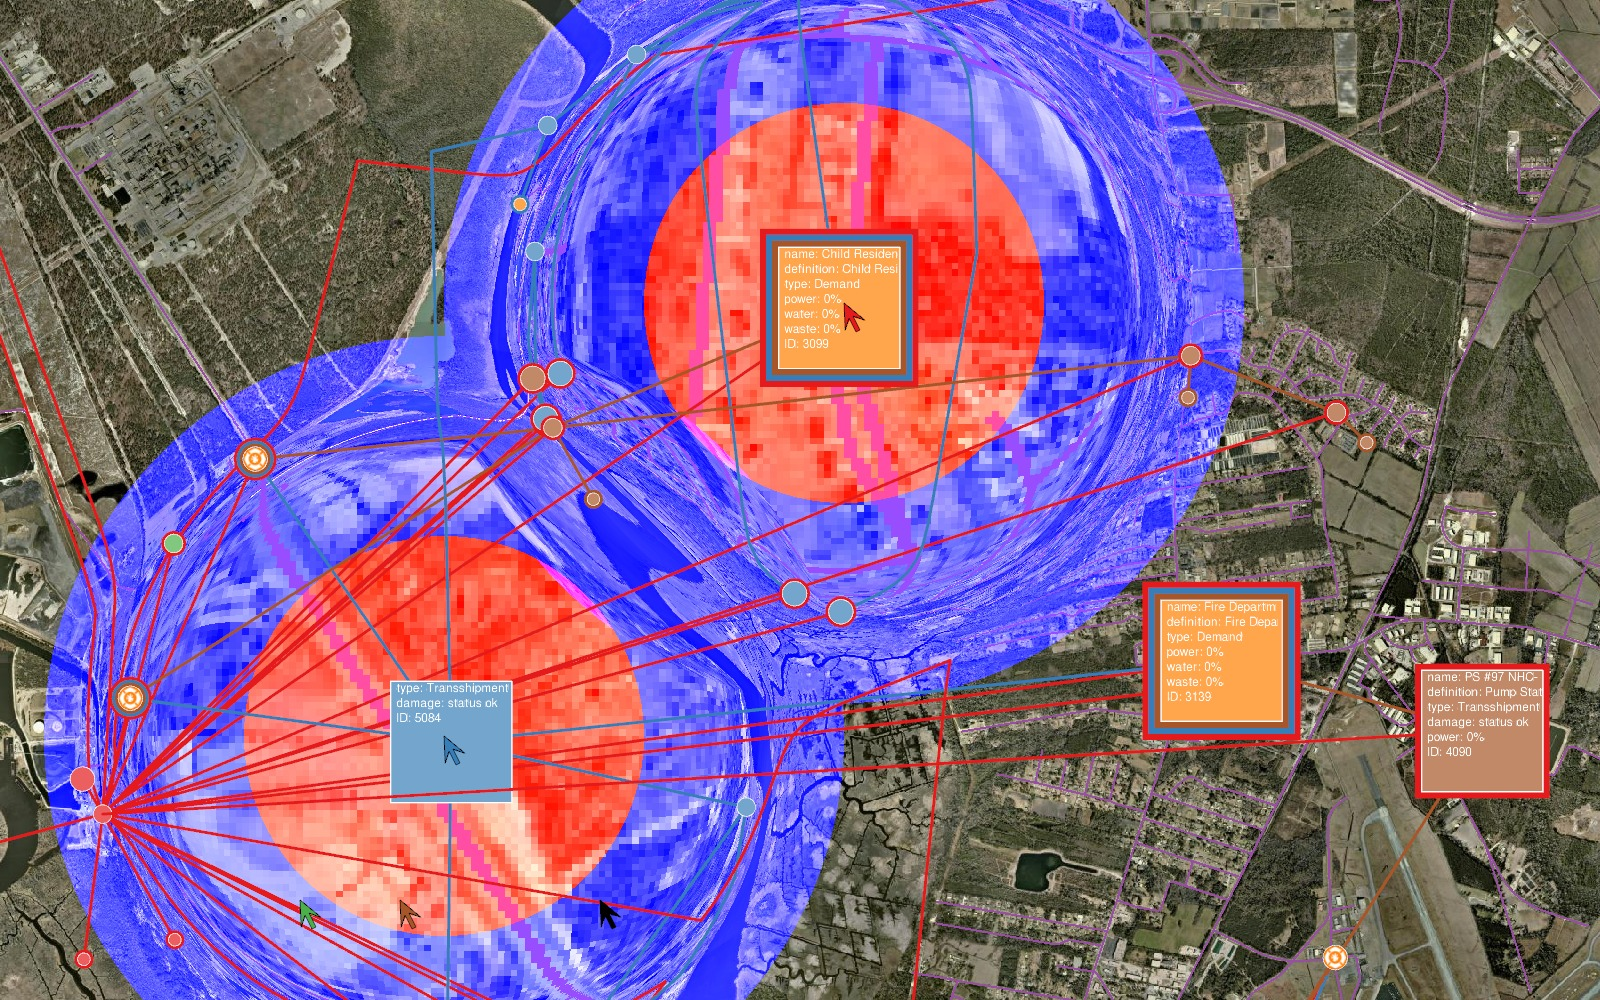
\includegraphics[width=0.49\linewidth]{img/problem_solving_20_20_color.jpg}
    \caption[Full Application with Two Areas of 6.7x Colored Linear Magnification]{An image showing the combined areas of magnification between two cursors. Each user is able to see their own region of interest in greater detail.}
    \label{fig:problem_solving}
\end{figure}

\begin{figure}[htp]\centering
    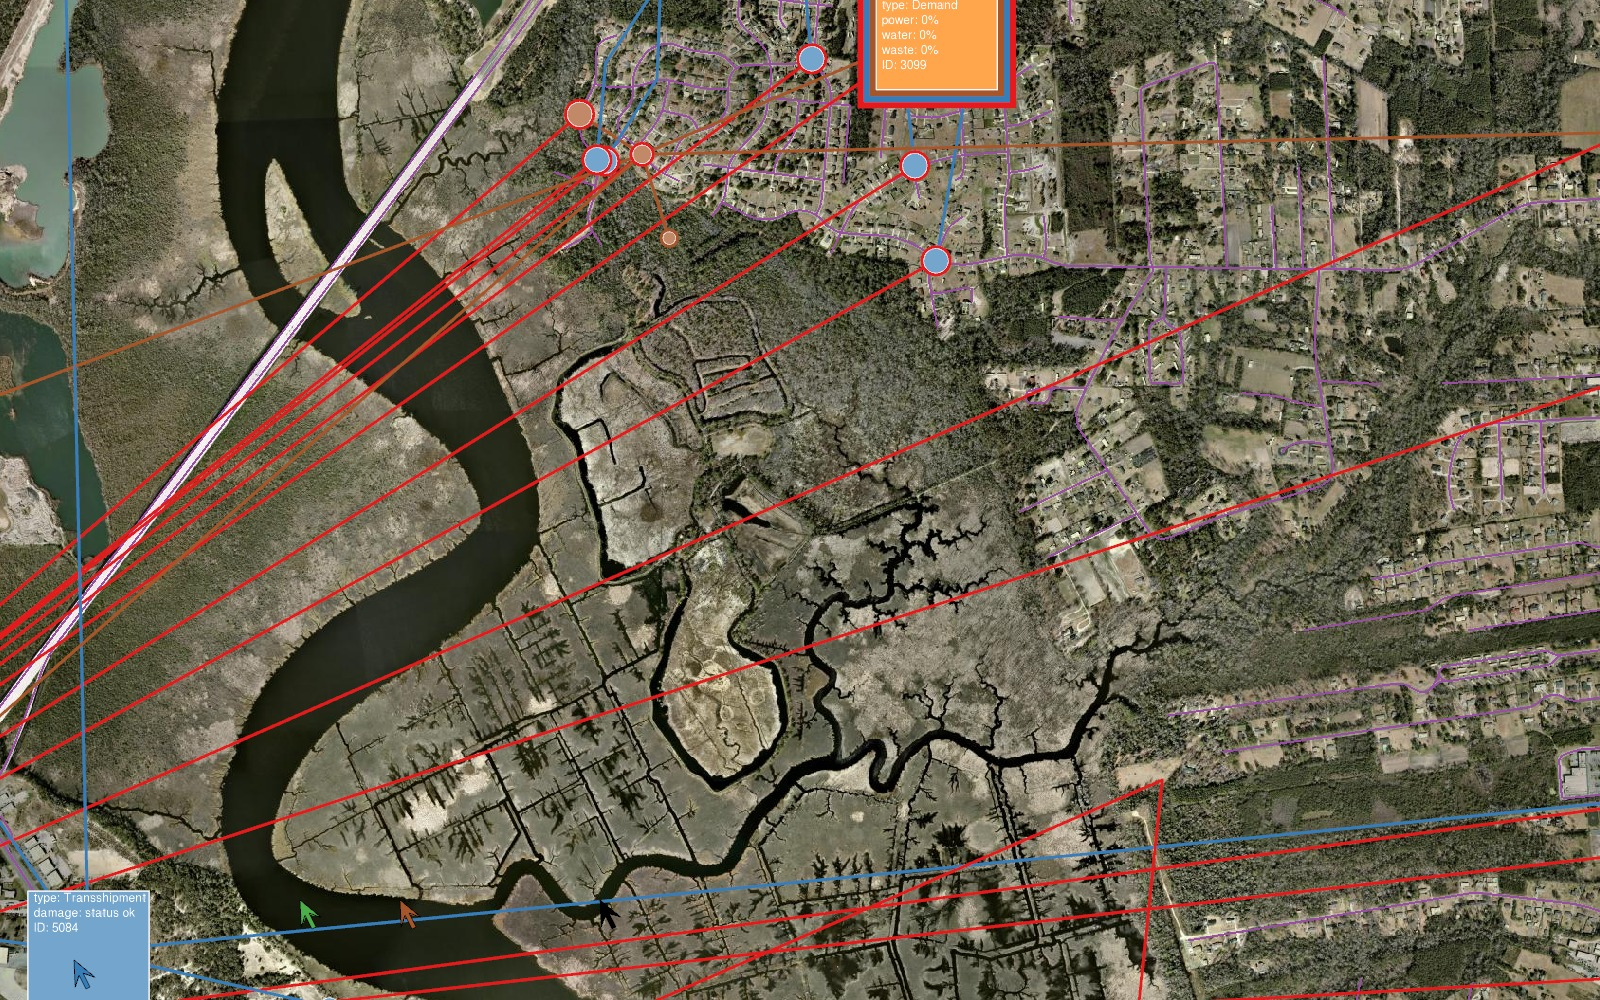
\includegraphics[width=0.90\linewidth]{img/normal_zoom.jpg}
    \caption[Full Application with Global Magnification]{The same nodes seen in Figure~\ref{fig:problem_solving}, with the maximum global magnification applied which has both nodes on screen. We cannot see the same level of local satellite imagery near the end points in question. }
    \label{fig:old_problem_solving}
\end{figure}

We can compare the focus plus context magnification seen in Figure~\ref{fig:problem_solving} to the global magnification seen in Figure~\ref{fig:old_problem_solving}. It is immediately apparent that the global magnification does not provide the same level in any way when compared to the focus plus context results. Many graph elements are now missing from this picture due to the global zoom, so it is difficult to see how these two nodes relate to other nodes within the graph.
This global magnification also fails to adequately show much geographic information about the area surrounding each of the expanded nodes.


Figure~\ref{fig:centered} shows a single cursor interacting with a single graph node and edge. If we examine the magnification of the satellite images and graph network, we can see that the node stays in the same geographic location, i.e.\ if this was a physical map, the node stays stuck to its position even when we fold the map to produce a magnification. This was the intended purpose of the magnification for both the satellite images and graph network, as it allows for users to see high magnification satellite data and interact with the system without performing a global
zoom. Unfortunately, because the nodes remain geographically rooted, interacting with graph elements becomes more difficult. The cursor still moves in screen space, despite covering more geographic space. The elements also move from their original position, requiring more hand-eye coordination to accurately interact with the elements. This problem is further exacerbated when higher levels of magnification are used, as the elements simply move around a cursor even faster.

\begin{figure}[htp]\centering
    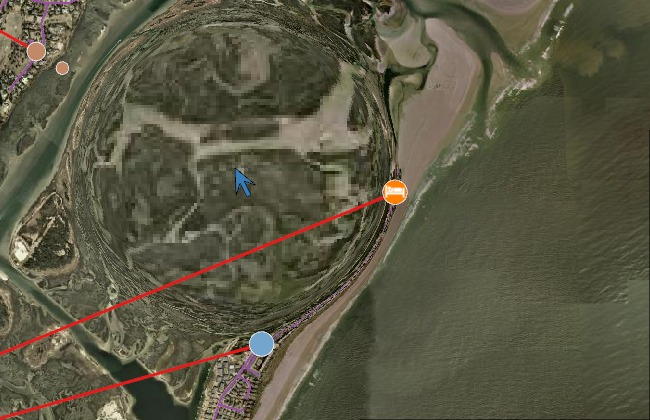
\includegraphics[width=0.40\linewidth]{img/12_edge_crop.jpg}
    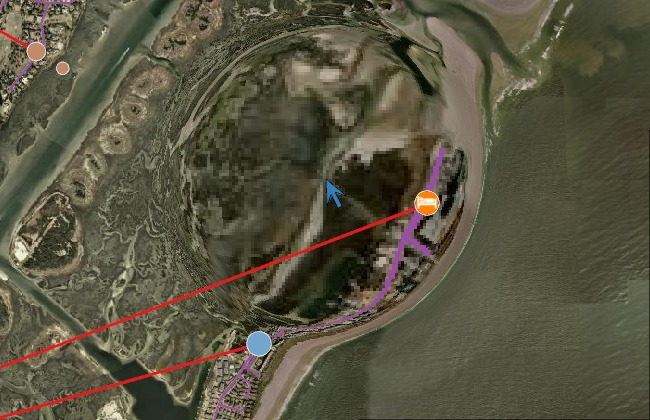
\includegraphics[width=0.40\linewidth]{img/12_mild_offset_crop.jpg}
    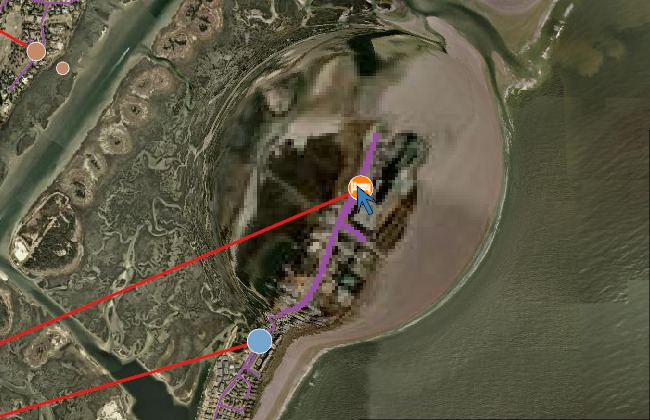
\includegraphics[width=0.40\linewidth]{img/12_center_crop.jpg}
    \caption[Node and Satellite Image Interaction with 3.1x Linear Magnification Centered on Node]{These images depict a single cursor trying to center itself on a particular node. There is some slight difficulty in this task, as the node changes position due to the magnification function. Currently, the cursor movement is relative to the original unmagnified screenspace, so with high magnification, the movement of the cursor is visually fast in the magnified region.}
    \label{fig:centered}
\end{figure}

\begin{figure}[htp]\centering
    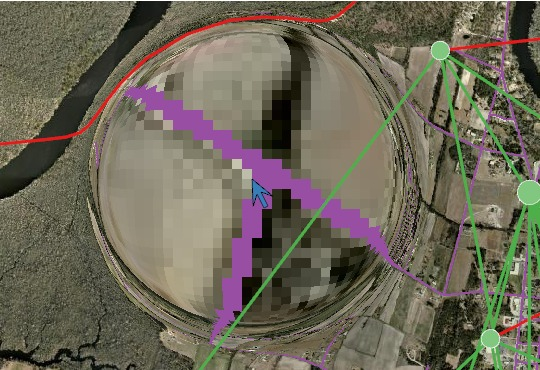
\includegraphics[width=0.90\linewidth]{img/p_vs_t_clip.jpg}
    \caption[Edge Differences]{An image showing that edges which have a defined path, such as red buried power lines, retain their geographic location during magnification and bend around the magnification region. This contrasts with the green communication edge which connects nodes with a straight line regardless of the magnification. }
    \label{fig:edge_differences}
\end{figure}

Certain edges within the system are defined to follow a specific path. These edges were subdivided into many smaller line segments to have the shape of the path retain its geographic location when magnified. This subdivision occurred on edges which were defined with more than two end points. This was simply a rough proof of concept, and can easily be extended to look for details within the edges themselves to perform this subdivision. An image displaying the visualization of two different
edges is seen in Figure~\ref{fig:edge_differences}. 

Finally, Figure~\ref{fig:ratio} shows the flexibility of the generated magnification functions for the application. As we increase the size of the linear magnification, the region of non-linear data becomes more distorted, resulting in data loss. When the linear and non-linear regions are the same size, we see that the satellite images and road network lose data completely, as the magnification function is no longer C0 continuous. The image with mostly linear magnification
but a slight amount of non-linear seems to provide the most benefit, as the data within the linear region is undistorted, and the global context of the data is still mostly retained.


\begin{figure}[htp]\centering
    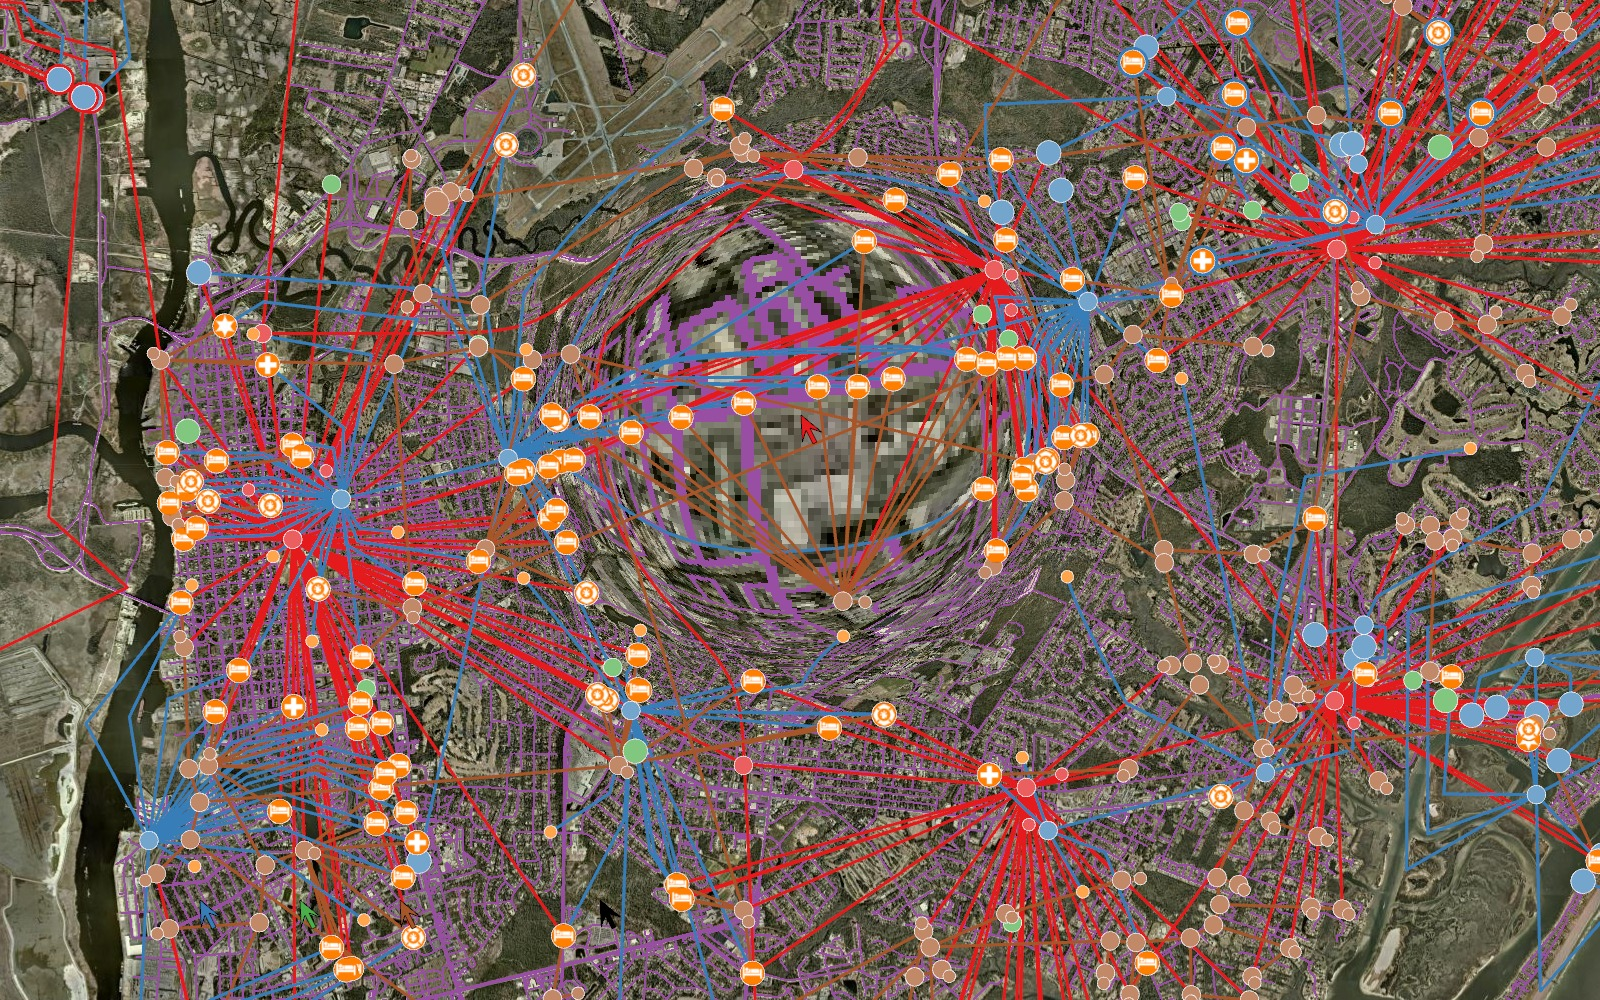
\includegraphics[width=0.40\linewidth]{img/20_no_linear.jpg}
    \includegraphics[width=0.40\linewidth]{img/20_no_linear_color.jpg}
    \vspace{3 mm}
    \includegraphics[width=0.40\linewidth]{img/20_one_quarter.jpg}
    \includegraphics[width=0.40\linewidth]{img/20_one_quarter_color.jpg}
    \vspace{3 mm}
    \includegraphics[width=0.40\linewidth]{img/20_half_linear.jpg}
    \includegraphics[width=0.40\linewidth]{img/20_half_linear_color.jpg}
    \vspace{3 mm}
    \includegraphics[width=0.40\linewidth]{img/20_three_quarter.jpg}
    \includegraphics[width=0.40\linewidth]{img/20_three_quarter_color.jpg}
    \vspace{3 mm}
    \includegraphics[width=0.40\linewidth]{img/20_only_linear.jpg}
    \includegraphics[width=0.40\linewidth]{img/20_only_linear_color.jpg}
    \caption[Various Inner and Outer Radius Ratios]{A series of images showing examples of different sized linear and non-linear magnification regions. As we increase the size of the linear region, the non-linear region becomes more and more distorted.}
    \label{fig:ratio}
\end{figure}
    

\section{Performance}
\label{section:performance_results}

Different aspects of the system were analyzed with regards to their performance. Each of the main individual systems: the satellite images, the road network, and the graph network were measured for the amount of time it took to complete a single render function of their respective data. 

For rendering the satellite images, we measured the amount of time it took to render to the FBO for a 1600 by 1000 resolution window\@. Figure~\ref{fig:satellite_graph} displays this information.  For the most part, rendering the satellite images takes less than 0.02 seconds no matter the number of tiles being rendered. Each tile is a 1024 by 1024 texture. The number of tiles on screen depends on the current level of detail of the overall application, as well as the positioning
within the application. The individual data points were simply measured by recording the amount of time a single render function call occurred, including the retrieval of the correct texture. The blue line in the graph shows the average amount of time it takes to render the satellite images with a specific number of tiles as the number of tiles increases.

\begin{figure}[htp]\centering
    \includegraphics[width=0.80\linewidth]{img/satellite_render_graph.jpg}
    \caption[Satellite Image Render Time Graph]{The blue line represents the average amount of time it takes to render a given number of tiles. The red dots are individual data points. The outliers are likely due to the time the simulation takes to load a new image when viewing a different part of the map that is not already loaded into the cache.}
    \label{fig:satellite_graph}
\end{figure}

Table~\ref{table:road_and_graph_render_time} shows the average render time for the road network and graph network. Currently, neither the graph network nor the road network vary in size, so we simply calculate the average time for rendering for the current status of the system. Both take a relatively insignificant amount of time to render, even though the road network has roughly 640,000 vertices and the graph network has approximately 60,000 vertices being rendered.

\begin{table}[htp]
    \begin{center}
        \caption[Road and Graph Network Average Render Time]{The average time it takes to perform a render of the different elements for the current state of the system.}
        \label{table:road_and_graph_render_time}
        \begin{tabular}[H]{l | c | c}
                                & Number of Elements    & Time (ms)   \\
            \hline
            Satellite Images    & Up to 15              & 4.954 \\
            Road Network        & 33664                 & 0.492 \\
            Graph Network       & 2563                  & 6.409 \\
        \end{tabular}
    \end{center}
\end{table}

In addition to the graph network being measured in terms of render performance, we recorded the amount of time it took to perform the magnification functions on the graph network, nodes and edges are treated equally within this calculation, so the total number of elements is simply the sum of nodes and edges within the system. This is seen Figures~\ref{fig:one_mouse_data},~\ref{fig:two_mouse_data} and~\ref{fig:three_mouse_data}.

\begin{figure}[htp] \centering
    \includegraphics[width=0.60\linewidth]{img/one_mouse_move.jpg}
    \caption[Graph Magnification Calculation Time for One Cursor]{The red circles represent individual data points for a given amount of graph elements. The blue line simply shows the average, but there are relatively few outliers, and the graph clearly shows that the correlation between the number of elements and the time required to perform the movement function is roughly linear.}
    \label{fig:one_mouse_data}
\end{figure}
\begin{figure} \centering
    \includegraphics[width=0.60\linewidth]{img/two_mouse_move.jpg}
    \caption[Graph Magnification Calculation Time for Two Cursors]{Like the previous figure, the correlation is roughly linear between the number of elements and the time required. Adding an additional cursor increases the rate of growth of the function.}
    \label{fig:two_mouse_data}
\end{figure}
\begin{figure}[htp] \centering
    \includegraphics[width=0.60\linewidth]{img/three_mouse_move.jpg}
    \caption[Graph Magnification Calculation Time for Three Cursors]{An additional cursor keeps the linear correlation between the number of elements and calculation time. We also see that the extra cursor further increases the growth rate of the function.}
    \label{fig:three_mouse_data}
\end{figure}

Currently, the system runs with 808 nodes and 1755 edges for a total of 2563 elements. Even with roughly ten times as many data elements, it only takes 0.08 seconds for one, two, or three cursors. Increasing the number of cursors within the system causes a linear growth in the amount of time it takes to perform the magnification. It may be possible to make this growth sub-linear by utilizing the existing quad-tree data structure. This was simulated by duplicating the elements within the graph network, as we do not have a dataset that contains more than 2563 elements. It is unlikely
that we would need work with a data set much bigger than 200,000 elements. Assuming that elements are evenly distributed, we would have a region that covers 100 times the area - resulting in a simulation for a region that would be handled by more than a single team of emergency response officials.

The gDEBugger application was also used to measure global aspects of the visualization's performance \cite{gdebugger_website}. Memory usage of the application can be seen in Table~\ref{table:memory}. Figure~\ref{fig:fps_graph} shows a graph of the frames per second (FPS) for the application over the first thirty seconds of runtime.

\begin{figure}[htp] \centering
    \includegraphics[width=0.80\linewidth]{img/FPS_graph.jpg}
    \caption[Overall Application FPS]{The red line shows that the average FPS over the first 20 seconds is 37.23 FPS\@. The initial low FPS is due to the application taking a few seconds to load data from the database which blocks all rendering.}
    \label{fig:fps_graph}
\end{figure}

The system maintains an interactive framerate, with only a few instances of the FPS dipping below 30. Even with these dips in framerate, this should not hinder the usage of the overall application, as users will probably not be continually interacting with the system.

\begin{table}[htp]
    \caption[Memory Usage]{The memory usage of the OpenGL relevant portions of the application is displayed. Textures take up approximately 50\% of the data being stored. Overall, the application uses a relatively small amount of GPU data, only 107 MB total.}
    \label{table:memory}
    \begin{center}
        \begin{tabular}[H]{l | r | c}
            Object Type     & Memory Size   & \# of Objects \\
            \hline
            Shaders         & 43 KB         & 32  \\
            Shading Programs& Insignificant & 13  \\
            VBOs            & 21956 KB      & 54  \\
            FBOs            & Insignificant & 1   \\
            Textures        & 49905 KB      & 17  \\
            Static Buffers  & 35941 KB      & 8   \\
            \hline
            Total           & 107845 KB     & 125 \\
        \end{tabular}
    \end{center}
\end{table}

The textures containing satellites are the biggest contributor of memory within the system, followed closely by the static buffers and the VBOs. We frequently update the texture and VBO data, so it may be prudent to try and reduce the amount of data being stored for VBOs. Because this application only takes up 107 MB of data on the GPU, it should run on pretty much any hardware. Dedicated GPUs usually have between 1 GB and 4 GB of memory, and integrated GPUs use the regular system RAM.

\section{Survey and Discussion}
\label{section:user_survey}

An informal survey of fellow students was performed for preliminary feedback on the changes proposed in Chapter~\ref{chapter:magnification} with regards to using the overall application. The different participants were given time to interact with the map for five minutes using the traditional methods of global zooming. After this time period passed, they used the new focus plus context system, and their opinions and thoughts about the two different methods of interaction were
recorded.

\begin{itemize}
    \item Magnification looks intuitive, seems like holding a magnifying glass.
    \item Magnification draws eyes to the magnified area.
    \item Cursor magnification instead of traditional zooming useful due to global information.

    \item Combined areas of magnification look weird, but unsure what should be displayed.

    \item With high magnification, mouse interaction is too sensitive.
    \item Some edges being magnified while others aren't is distracting.
    \item Difficult to click on elements due to how the nodes move around, try applying a different effect instead of just moving them.
\end{itemize}

The fact that the participants found the visualization helpful was expected due to the application requiring a global overview of the entire data to formulate solutions. The responses related to the actual interaction with the system were surprising. Due to my familiarity with the system, I did not notice that graph elements changing their screen position was initially a difficult concept to grasp, as the elements initially move away as you approach them. The oversensitivity of the interaction was expected, as it was difficult to control even when debugging.

In a formal study, it is  important to get quantitative data about user interaction with the system and the overall usefulness of the visualization. By logging the actions that a user takes while interacting with this system, an experiment could be designed to measure the number of actions a user needs to take to perform a task within the system. We could measure the amount of distance that the
mouse cursor travels and count the number of actions performed to quantify the usability of the entire visualization. Having lower values for both would indicate that the user was able to see more data and was assisted by the overall system. 

\section{Summary}
\label{section:results_summary}

This chapter presented a series of figures showing the magnification of the satellite images and graph network with single and multiple cursors interacting with the system. We also discussed various performance statistics related to rendering and performing magnification operations on the CPU\@. Finally, we detailed the results of a brief survey of inexperienced users regarding the visual effects of the system and their interaction. The following chapter will discuss possible future
work stemming from this thesis.



%%%%%%%%%%%%%%%%%%%%%%%%%%%%%%%%%%%%%%%%%%%%%%%%%%%%%%%%%%%%%%%%%%% 
%                                                                 %
%                           FUTUREWORK                            %
%                                                                 %
%%%%%%%%%%%%%%%%%%%%%%%%%%%%%%%%%%%%%%%%%%%%%%%%%%%%%%%%%%%%%%%%%%% 
 
% \specialhead{FUTUREWORK}
\chapter{FUTURE WORK AND CONCLUSION}
\label{chapter:future_work}

The previous chapter presented the resulting visualization from applying the magnification functions to the graph network and satellite images. The overall performance of the application was also measured to ascertain the viability of using this visualization for larger datasets. This chapter will present a few areas of possible improvement for the current implementation with regards to visual results and algorithm performance.

\section{Satellite Images}
\label{section:future_satellite_images}

The current method of performing linear magnification on the satellite images does not provide the same level of detail of the resulting image as an equivalent global zoom does. This is due to the magnification spreading a relatively small number of texture coordinates over a large area of screen space. Ideally, we would use a method similar to mipmapping where we load the higher resolution textures into GPU memory and use that to provide a greater amount of detail for the magnified
areas. This method was proposed by Keahey as Seamless Multi-Level Views \cite{Keahey1998}.

\begin{figure} \centering
    \includegraphics[width=0.50\linewidth]{img/artifacts_clipped.jpg}
    \caption[Satellite Image Magnification Artifacts]{Individual pixels are currently seen with a 72x linear zoom.}
    \label{fig:artifacts_clipped}
\end{figure}

There are a few problems with directly implementing such a technique. There is a limited amount of data that can be stored at any particular resolution on the GPU\@. The amount of memory stored on a GPU averages at about 2 GB\@. As stated previously, the FBO texture takes up approximately 4.5 MB with the application running at a 1600 by 1000 resolution. The FBO is currently used to store any data that is not immediately rendered as textures. 2D textures are limited within OpenGL by their
larger dimension, this value ranges from 1024 to 16384, depending on the hardware. If we have twice the level of detail of a region, we must take up four times as much data in the resulting texture if we wish to store the same geographic coordinates as the lower level of detail image. This magnified region could be generated as the cursors move around the application, but that requires the operations to be fast enough
to calculate every possible discrete level of detail that the cursors can use. The current cursors move to fast with respect to geographic positions, so once this has been addressed, the system would not need to update these extra regions as often. We could also use the lower resolution texture as an option until the higher resolution one has been made available.

While seeing the individual pixels helps the user understand how much they are magnifying the source texture, it obscures any finer details about the geography that might be useful information. Being able to see more detail is the priority of performing magnification. Other effects can be added to help indicate the intensity of a magnification, as suggested by Keahey \cite{Keahey1998}.

The road networks, similar to the satellite images, are also heavily pixelated in the resulting magnification. This can be fixed by simply rendering the road network to the screen instead of to the FBO. 

\begin{figure} \centering
    \includegraphics[width=0.50\linewidth]{img/aliasing_clip.jpg}
    \caption[Road Network Artifacts]{The aliasing of the road network is seen due to the 17.4x linear zoom.}
    \label{fig:aliasing_clipped}
\end{figure}

Combined magnification regions caused by overlapping mouse cursors for satellite images produce some odd results. An example is seen in Figure~\ref{fig:distortion_clipped}. It is unclear what should happen when two regions are combined for our applications, it may be correct to prevent different cursors from interacting with each other to avoid creating any sort of extreme satellite distortion. A few options for combining areas of magnification were presented by Keahey and Robertson, including weighted
averages and maximal ray clipping \cite{Keahey1996}.

\begin{figure} \centering
    \includegraphics[width=0.50\linewidth]{img/added_distortion_clip.jpg}
    \caption[Combined Satellite Distortion]{An image showing two combined areas of 6.7x magnification. The continuous river south of the cursors does not contain a branch in the original image.}
    \label{fig:distortion_clipped}
\end{figure}

\section{Graph Network}
\label{section:future_graph_network}

Combined areas of magnification do not currently result in graph elements being placed in the same geographic location due to an algorithmic error. This is due to a difference in the premise behind the texture magnification and the graph magnification. The algorithm for texture magnification calculates what geographic data should go at a particular screen location, while the graph magnification tells graph elements to move to a screen location. To move the elements of the graph correctly, we must apply the movement operation to the graph multiple times for each cursor until the same result is obtained twice. 

We can avoid the incorrect placement of graph elements by changing the interaction between areas of magnification. When areas of magnification overlap, we can have the application respond by having the cursors stay in the same screen position but display different geographic and graph information. Another possibility is performing magnification on the convex shape or line formed by elements whose areas of magnification overlap.

As mentioned previously in Chapter~\ref{chapter:results}, the graph movement operations are inefficient for large amounts of data. The current set of graph operations rely on a quad tree implementation which could be used to avoid measuring the distance to every element within the graph. While this quad tree implementation would not improve performance where a large amount of nodes are in a single area, the fact that the data is geographic ensures that this situation is rare.

\section{Conclusion}
\label{section:conclusion}

Creating a focus plus context visualization of data is highly dependent on what information needs to be displayed. For the Infrastructure Visualization, we opt to use a region of non-linear magnification surrounding a region of linear magnification to keep as much context of the data as possible. This thesis explained the necessary changes to the existing visualization to transition to modern OpenGL to perform these functions on our data. We presented techniques for applying
this magnification to both the satellite data and the geographically-based graph data to ensure that the data remained consistent visually. These functions are currently
efficient enough to support a system with 20,000 elements and run in real time.

\specialhead{References}

\bibliography{IEEEabrv,research}
\bibliographystyle{ieeetran}
% \include{Bibliography} 	% bibliography
%\include{rpiapp} 	% appendix
\end{document}
